\documentclass[twoside]{book}

% Packages required by doxygen
\usepackage{fixltx2e}
\usepackage{calc}
\usepackage{doxygen}
\usepackage{graphicx}
\usepackage[utf8]{inputenc}
\usepackage{makeidx}
\usepackage{multicol}
\usepackage{multirow}
\PassOptionsToPackage{warn}{textcomp}
\usepackage{textcomp}
\usepackage[nointegrals]{wasysym}
\usepackage[table]{xcolor}

% Font selection
\usepackage[T1]{fontenc}
\usepackage{mathptmx}
\usepackage[scaled=.90]{helvet}
\usepackage{courier}
\usepackage{amssymb}
\usepackage{sectsty}
\renewcommand{\familydefault}{\sfdefault}
\allsectionsfont{%
  \fontseries{bc}\selectfont%
  \color{darkgray}%
}
\renewcommand{\DoxyLabelFont}{%
  \fontseries{bc}\selectfont%
  \color{darkgray}%
}
\newcommand{\+}{\discretionary{\mbox{\scriptsize$\hookleftarrow$}}{}{}}

% Page & text layout
\usepackage{geometry}
\geometry{%
  a4paper,%
  top=2.5cm,%
  bottom=2.5cm,%
  left=2.5cm,%
  right=2.5cm%
}
\tolerance=750
\hfuzz=15pt
\hbadness=750
\setlength{\emergencystretch}{15pt}
\setlength{\parindent}{0cm}
\setlength{\parskip}{0.2cm}
\makeatletter
\renewcommand{\paragraph}{%
  \@startsection{paragraph}{4}{0ex}{-1.0ex}{1.0ex}{%
    \normalfont\normalsize\bfseries\SS@parafont%
  }%
}
\renewcommand{\subparagraph}{%
  \@startsection{subparagraph}{5}{0ex}{-1.0ex}{1.0ex}{%
    \normalfont\normalsize\bfseries\SS@subparafont%
  }%
}
\makeatother

% Headers & footers
\usepackage{fancyhdr}
\pagestyle{fancyplain}
\fancyhead[LE]{\fancyplain{}{\bfseries\thepage}}
\fancyhead[CE]{\fancyplain{}{}}
\fancyhead[RE]{\fancyplain{}{\bfseries\leftmark}}
\fancyhead[LO]{\fancyplain{}{\bfseries\rightmark}}
\fancyhead[CO]{\fancyplain{}{}}
\fancyhead[RO]{\fancyplain{}{\bfseries\thepage}}
\fancyfoot[LE]{\fancyplain{}{}}
\fancyfoot[CE]{\fancyplain{}{}}
\fancyfoot[RE]{\fancyplain{}{\bfseries\scriptsize Generated on Fri Dec 5 2014 11\+:36\+:48 for fctransfer by Doxygen }}
\fancyfoot[LO]{\fancyplain{}{\bfseries\scriptsize Generated on Fri Dec 5 2014 11\+:36\+:48 for fctransfer by Doxygen }}
\fancyfoot[CO]{\fancyplain{}{}}
\fancyfoot[RO]{\fancyplain{}{}}
\renewcommand{\footrulewidth}{0.4pt}
\renewcommand{\chaptermark}[1]{%
  \markboth{#1}{}%
}
\renewcommand{\sectionmark}[1]{%
  \markright{\thesection\ #1}%
}

% Indices & bibliography
\usepackage{natbib}
\usepackage[titles]{tocloft}
\setcounter{tocdepth}{3}
\setcounter{secnumdepth}{5}
\makeindex

% Custom commands
\newcommand{\clearemptydoublepage}{%
  \newpage{\pagestyle{empty}\cleardoublepage}%
}


%===== C O N T E N T S =====

\begin{document}

% Titlepage & ToC
\pagenumbering{roman}
\begin{titlepage}
\vspace*{7cm}
\begin{center}%
{\Large fctransfer \\[1ex]\large 0.\+3-\/44 }\\
\vspace*{1cm}
{\large Generated by Doxygen 1.8.7}\\
\vspace*{0.5cm}
{\small Fri Dec 5 2014 11:36:48}\\
\end{center}
\end{titlepage}
\clearemptydoublepage
\tableofcontents
\clearemptydoublepage
\pagenumbering{arabic}

%--- Begin generated contents ---
\chapter{Java\+Doc A\+P\+I Markup for fctransfer}
\label{index}\section*{fctransfer }

Basic transfer (upload/download) functions to easily allow simpler tools to share config, content, and data.

This project is taken from fctools' section that allows it to checksum-\/upload a large data archive using only a U\+R\+L and a filename.

For example, given a target U\+R\+L ({\tt ftp\+://scott\+:tiger@ftp.\+example.\+com/sub/dir/}) and one or more files (ie data.\+zip), the library\+: 1) calculates a checksum 2) uploads the checksum as \{file\}.sum (in our example, a data.\+zip.\+sum file would be sent) 3) uploads the file (in our example, data.\+zip)

The uploaded checksum intentionally matches the checksum file used in ages-\/old traditional \char`\"{}sum\char`\"{} command; this is the same as the \char`\"{}cksum\char`\"{} command.

An additional intention of sharing this content is to\+: 1) reduce the time it takes Y\+O\+U, the next developer, in uploading/sharing content 2) emphasize better practices\+: checksums, people, they're really cool things 3) expand to provide an interface to additional upload U\+R\+L protocols\+: cifs\+://, etc.

Please post your enhancements as pull-\/requests! If I'm your upstream, share upwards! 
\chapter{R\+E\+A\+D\+M\+E}
\label{md_htdocs_README}
\input{md_htdocs_README}
\chapter{Hierarchical Index}
\section{Class Hierarchy}
This inheritance list is sorted roughly, but not completely, alphabetically\-:\begin{DoxyCompactList}
\item Exception\begin{DoxyCompactList}
\item \contentsline{section}{File\-Transfer\-Winch.\-File\-Transfer\-Winch\-Exception}{\pageref{classorg_1_1smallfoot_1_1filexfer_1_1FileTransferWinch_1_1FileTransferWinchException}}{}
\begin{DoxyCompactList}
\item \contentsline{section}{File\-Transfer\-Winch.\-File\-Transfer\-Aborted\-Exception}{\pageref{classorg_1_1smallfoot_1_1filexfer_1_1FileTransferWinch_1_1FileTransferAbortedException}}{}
\item \contentsline{section}{File\-Transfer\-Winch.\-File\-Transfer\-Data\-Transfer\-Exception}{\pageref{classorg_1_1smallfoot_1_1filexfer_1_1FileTransferWinch_1_1FileTransferDataTransferException}}{}
\begin{DoxyCompactList}
\item \contentsline{section}{File\-Transfer\-Winch.\-File\-Transfer\-Checksum\-Mismatch\-Exception}{\pageref{classorg_1_1smallfoot_1_1filexfer_1_1FileTransferWinch_1_1FileTransferChecksumMismatchException}}{}
\end{DoxyCompactList}
\item \contentsline{section}{File\-Transfer\-Winch.\-File\-Transfer\-Illegal\-F\-S\-M\-Reply\-Exception}{\pageref{classorg_1_1smallfoot_1_1filexfer_1_1FileTransferWinch_1_1FileTransferIllegalFSMReplyException}}{}
\end{DoxyCompactList}
\end{DoxyCompactList}
\item \contentsline{section}{File\-Transfer\-Winch}{\pageref{classorg_1_1smallfoot_1_1filexfer_1_1FileTransferWinch}}{}
\begin{DoxyCompactList}
\item \contentsline{section}{Apache\-Commons\-Net\-S\-F\-T\-P}{\pageref{classorg_1_1smallfoot_1_1filexfer_1_1ApacheCommonsNetSFTP}}{}
\item \contentsline{section}{F\-T\-P4\-J}{\pageref{classorg_1_1smallfoot_1_1filexfer_1_1FTP4J}}{}
\end{DoxyCompactList}
\item U\-R\-L\-Connection\begin{DoxyCompactList}
\item \contentsline{section}{S\-F\-T\-P\-U\-R\-L\-Connection}{\pageref{classorg_1_1smallfoot_1_1filexfer_1_1sftp_1_1SFTPURLConnection}}{}
\end{DoxyCompactList}
\item U\-R\-L\-Stream\-Handler\begin{DoxyCompactList}
\item \contentsline{section}{Handler}{\pageref{classorg_1_1smallfoot_1_1filexfer_1_1sftp_1_1Handler}}{}
\end{DoxyCompactList}
\item \contentsline{section}{version}{\pageref{classorg_1_1smallfoot_1_1transfer_1_1version}}{}
\end{DoxyCompactList}

\chapter{Data Structure Index}
\section{Data Structures}
Here are the data structures with brief descriptions\-:\begin{DoxyCompactList}
\item\contentsline{section}{{\bf Apache\-Commons\-Net\-S\-F\-T\-P} \\*Using Apache Commons-\/net-\/ssh, based on the S\-F\-T\-P\-Upload example at {\tt https\-://commons-\/net-\/ssh.\-googlecode.\-com/svn-\/history/r204/src/main/java/examples/ssh/\-S\-F\-T\-P\-Upload.\-java} , upload a file }{\pageref{classorg_1_1smallfoot_1_1filexfer_1_1ApacheCommonsNetSFTP}}{}
\item\contentsline{section}{{\bf File\-Transfer\-Winch.\-File\-Transfer\-Aborted\-Exception} \\*This exception indicates that transfer was aborted; I have not yet clarified in the A\-P\-I whether this exception would take precidence over \doxyref{File\-Transfer\-Data\-Transfer\-Exception}{p.}{classorg_1_1smallfoot_1_1filexfer_1_1FileTransferWinch_1_1FileTransferDataTransferException} if both occur, or a \doxyref{File\-Transfer\-Data\-Transfer\-Exception}{p.}{classorg_1_1smallfoot_1_1filexfer_1_1FileTransferWinch_1_1FileTransferDataTransferException} causes a \doxyref{File\-Transfer\-Aborted\-Exception}{p.}{classorg_1_1smallfoot_1_1filexfer_1_1FileTransferWinch_1_1FileTransferAbortedException} }{\pageref{classorg_1_1smallfoot_1_1filexfer_1_1FileTransferWinch_1_1FileTransferAbortedException}}{}
\item\contentsline{section}{{\bf File\-Transfer\-Winch.\-File\-Transfer\-Checksum\-Mismatch\-Exception} \\*This exception alerts to the specific Data Transfer issuesuch that the receiver's checksum confirmation did not match the sender .. }{\pageref{classorg_1_1smallfoot_1_1filexfer_1_1FileTransferWinch_1_1FileTransferChecksumMismatchException}}{}
\item\contentsline{section}{{\bf File\-Transfer\-Winch.\-File\-Transfer\-Data\-Transfer\-Exception} \\*This exception alerts to issues during transfer of data\-: connection lost, etc .. }{\pageref{classorg_1_1smallfoot_1_1filexfer_1_1FileTransferWinch_1_1FileTransferDataTransferException}}{}
\item\contentsline{section}{{\bf File\-Transfer\-Winch.\-File\-Transfer\-Illegal\-F\-S\-M\-Reply\-Exception} \\*This exception indicates that the underlying Finite State Machine received an unexpected reply, and has no next-\/state in the conversation }{\pageref{classorg_1_1smallfoot_1_1filexfer_1_1FileTransferWinch_1_1FileTransferIllegalFSMReplyException}}{}
\item\contentsline{section}{{\bf File\-Transfer\-Winch} }{\pageref{classorg_1_1smallfoot_1_1filexfer_1_1FileTransferWinch}}{}
\item\contentsline{section}{{\bf File\-Transfer\-Winch.\-File\-Transfer\-Winch\-Exception} \\*A base collector exception\-: \char`\"{}there was some exception in the File\-Transfer\-Winch class\char`\"{}; typically, more meaning and/or usefulness is reached by catching specific subclasses of this exception }{\pageref{classorg_1_1smallfoot_1_1filexfer_1_1FileTransferWinch_1_1FileTransferWinchException}}{}
\item\contentsline{section}{{\bf F\-T\-P4\-J} }{\pageref{classorg_1_1smallfoot_1_1filexfer_1_1FTP4J}}{}
\item\contentsline{section}{{\bf Handler} }{\pageref{classorg_1_1smallfoot_1_1filexfer_1_1sftp_1_1Handler}}{}
\item\contentsline{section}{{\bf S\-F\-T\-P\-U\-R\-L\-Connection} }{\pageref{classorg_1_1smallfoot_1_1filexfer_1_1sftp_1_1SFTPURLConnection}}{}
\item\contentsline{section}{{\bf version} }{\pageref{classorg_1_1smallfoot_1_1transfer_1_1version}}{}
\end{DoxyCompactList}

\chapter{File Index}
\section{File List}
Here is a list of all documented files with brief descriptions\+:\begin{DoxyCompactList}
\item\contentsline{section}{java/{\bfseries Apache\+Commons\+Net\+S\+F\+T\+P.\+java} }{\pageref{ApacheCommonsNetSFTP_8java}}{}
\item\contentsline{section}{java/{\bfseries File\+Transfer\+Winch.\+java} }{\pageref{FileTransferWinch_8java}}{}
\item\contentsline{section}{java/{\bfseries F\+T\+P4\+J.\+java} }{\pageref{FTP4J_8java}}{}
\item\contentsline{section}{java/{\bf version.\+java} }{\pageref{version_8java}}{}
\item\contentsline{section}{java/{\bf Winch\+Factory.\+java} }{\pageref{WinchFactory_8java}}{}
\item\contentsline{section}{java/sftp/{\bf Handler.\+java} }{\pageref{Handler_8java}}{}
\item\contentsline{section}{java/sftp/{\bf S\+F\+T\+P\+U\+R\+L\+Connection.\+java} }{\pageref{SFTPURLConnection_8java}}{}
\end{DoxyCompactList}

\chapter{Data Structure Documentation}
\section{Apache\+Commons\+Net\+S\+F\+T\+P Class Reference}
\label{classorg_1_1smallfoot_1_1filexfer_1_1ApacheCommonsNetSFTP}\index{Apache\+Commons\+Net\+S\+F\+T\+P@{Apache\+Commons\+Net\+S\+F\+T\+P}}


Using Apache Commons-\/net-\/ssh, based on the S\+F\+T\+P\+Upload example at {\tt https\+://commons-\/net-\/ssh.\+googlecode.\+com/svn-\/history/r204/src/main/java/examples/ssh/\+S\+F\+T\+P\+Upload.\+java} , upload a file.  




Inheritance diagram for Apache\+Commons\+Net\+S\+F\+T\+P\+:\nopagebreak
\begin{figure}[H]
\begin{center}
\leavevmode
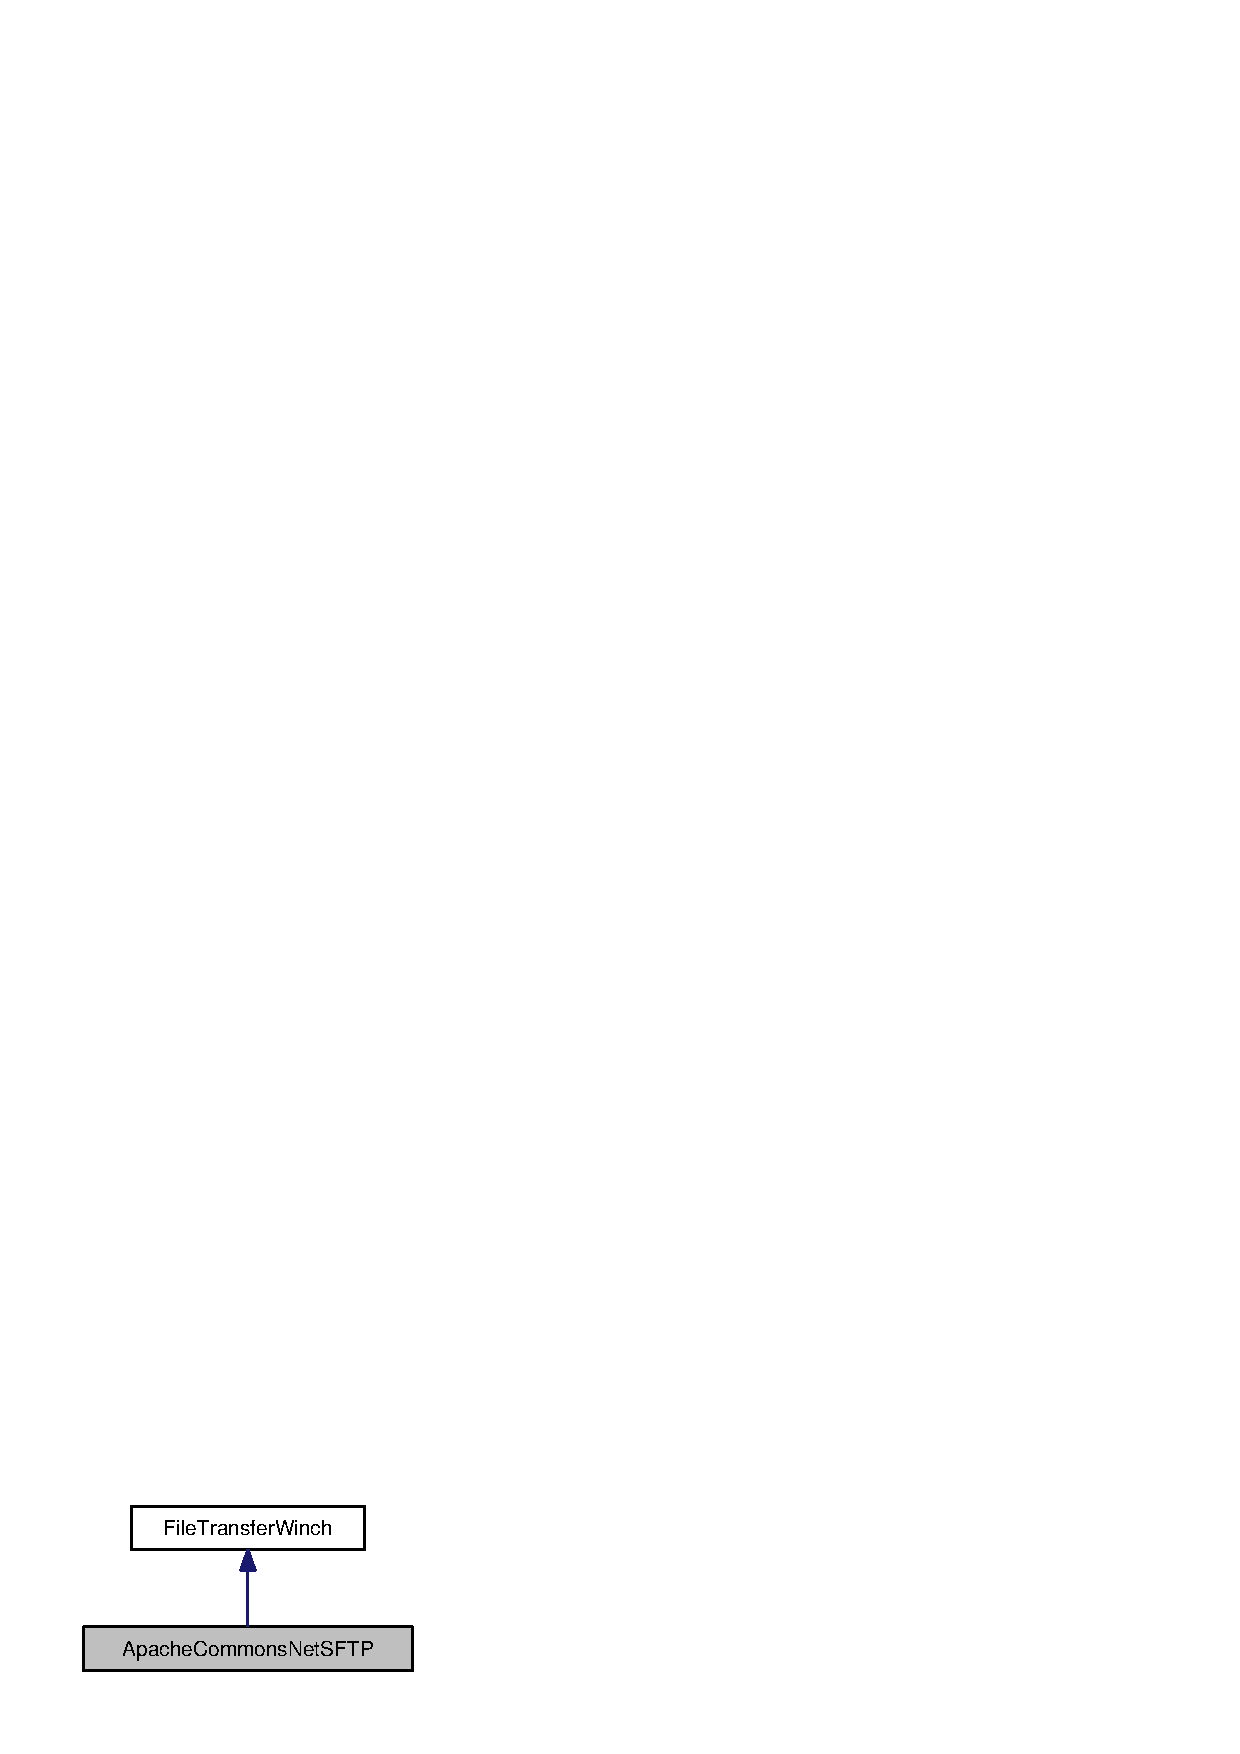
\includegraphics[width=202pt]{classorg_1_1smallfoot_1_1filexfer_1_1ApacheCommonsNetSFTP__inherit__graph}
\end{center}
\end{figure}


Collaboration diagram for Apache\+Commons\+Net\+S\+F\+T\+P\+:\nopagebreak
\begin{figure}[H]
\begin{center}
\leavevmode
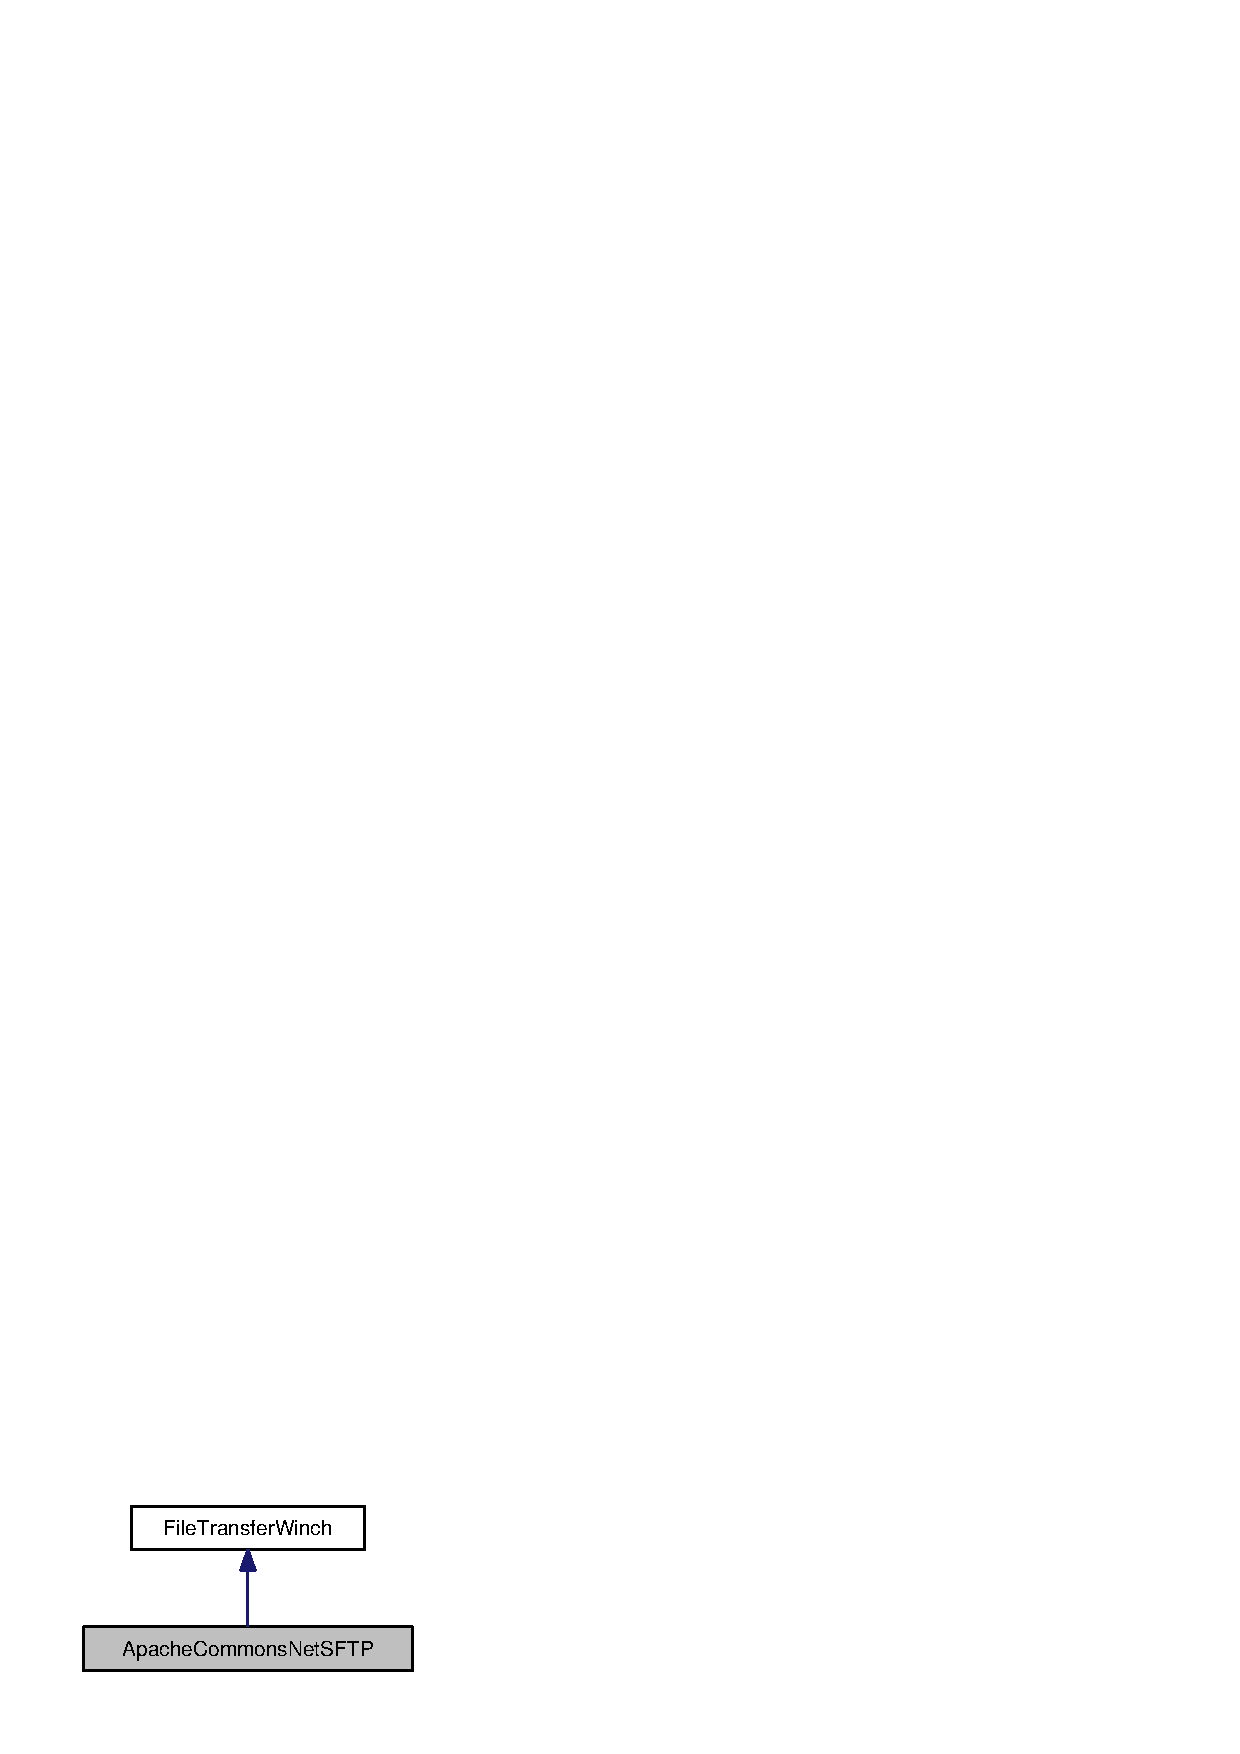
\includegraphics[width=202pt]{classorg_1_1smallfoot_1_1filexfer_1_1ApacheCommonsNetSFTP__coll__graph}
\end{center}
\end{figure}
\subsection*{Public Member Functions}
\begin{DoxyCompactItemize}
\item 
{\bfseries Apache\+Commons\+Net\+S\+F\+T\+P} (java.\+net.\+U\+R\+L u)\label{classorg_1_1smallfoot_1_1filexfer_1_1ApacheCommonsNetSFTP_a67d38a2fe0500ee93a9613fc011497b4}

\item 
String {\bfseries name} ()\label{classorg_1_1smallfoot_1_1filexfer_1_1ApacheCommonsNetSFTP_afa2149aced9d90555f788dfc81c23d15}

\item 
boolean {\bf upload} (File file, Vector$<$ String $>$ upload\+Notify)  throws File\+Transfer\+Winch\+Exception     
\begin{DoxyCompactList}\small\item\em Attempt an upload to the remote server. \end{DoxyCompactList}\end{DoxyCompactItemize}
\subsection*{Static Public Member Functions}
\begin{DoxyCompactItemize}
\item 
static String[$\,$] {\bf examples} (java.\+net.\+U\+R\+L url)
\begin{DoxyCompactList}\small\item\em list one or more example U\+R\+Ls showing the available upload/download protocols \end{DoxyCompactList}\item 
static boolean {\bfseries handles} (java.\+net.\+U\+R\+L u)\label{classorg_1_1smallfoot_1_1filexfer_1_1ApacheCommonsNetSFTP_a4ef8d35ab128080eb511f7e26cd7ab7b}

\end{DoxyCompactItemize}
\subsection*{Additional Inherited Members}


\subsection{Detailed Description}
Using Apache Commons-\/net-\/ssh, based on the S\+F\+T\+P\+Upload example at {\tt https\+://commons-\/net-\/ssh.\+googlecode.\+com/svn-\/history/r204/src/main/java/examples/ssh/\+S\+F\+T\+P\+Upload.\+java} , upload a file. 

Definition at line 28 of file Apache\+Commons\+Net\+S\+F\+T\+P.\+java.



\subsection{Member Function Documentation}
\index{org\+::smallfoot\+::filexfer\+::\+Apache\+Commons\+Net\+S\+F\+T\+P@{org\+::smallfoot\+::filexfer\+::\+Apache\+Commons\+Net\+S\+F\+T\+P}!examples@{examples}}
\index{examples@{examples}!org\+::smallfoot\+::filexfer\+::\+Apache\+Commons\+Net\+S\+F\+T\+P@{org\+::smallfoot\+::filexfer\+::\+Apache\+Commons\+Net\+S\+F\+T\+P}}
\subsubsection[{examples}]{\setlength{\rightskip}{0pt plus 5cm}static String [$\,$] examples (
\begin{DoxyParamCaption}
\item[{java.\+net.\+U\+R\+L}]{url}
\end{DoxyParamCaption}
)\hspace{0.3cm}{\ttfamily [inline]}, {\ttfamily [static]}}\label{classorg_1_1smallfoot_1_1filexfer_1_1ApacheCommonsNetSFTP_ad6f50b0642401b9d8a38893ccc852bdf}


list one or more example U\+R\+Ls showing the available upload/download protocols 


\begin{DoxyParams}{Parameters}
{\em url} & a sample U\+R\+L showing user/pass/pathname \\
\hline
\end{DoxyParams}
\begin{DoxyReturn}{Returns}
array of examples using that U\+R\+L 
\end{DoxyReturn}


Definition at line 52 of file Apache\+Commons\+Net\+S\+F\+T\+P.\+java.



Referenced by Winch\+Factory.\+get\+Winch\+Examples().

\index{org\+::smallfoot\+::filexfer\+::\+Apache\+Commons\+Net\+S\+F\+T\+P@{org\+::smallfoot\+::filexfer\+::\+Apache\+Commons\+Net\+S\+F\+T\+P}!upload@{upload}}
\index{upload@{upload}!org\+::smallfoot\+::filexfer\+::\+Apache\+Commons\+Net\+S\+F\+T\+P@{org\+::smallfoot\+::filexfer\+::\+Apache\+Commons\+Net\+S\+F\+T\+P}}
\subsubsection[{upload}]{\setlength{\rightskip}{0pt plus 5cm}boolean upload (
\begin{DoxyParamCaption}
\item[{File}]{file, }
\item[{Vector$<$ String $>$}]{upload\+Notify}
\end{DoxyParamCaption}
) throws {\bf File\+Transfer\+Winch\+Exception}\hspace{0.3cm}{\ttfamily [inline]}}\label{classorg_1_1smallfoot_1_1filexfer_1_1ApacheCommonsNetSFTP_afa3dfccec4b989cafc56103eb1ee82a6}


Attempt an upload to the remote server. 

Initially very basic, this can be extended for all the intelligence we need to get data through.

This function, given a filename, connects to an F\+T\+P server and attempts to store the file. Initially the username and password are defaulted to those usable to upload from P\+A\+K\+\_\+\+R\+E\+D, but later (when i can look at U\+R\+L factories) this can be extended. The capability will be preserved to give the function a list of statuses and a position so that a later threaded design can try a number of uploads in parallel, ditching all but the most efficient\+: on connection, so status-\/indiciates; on successful 1-\/k upload with a temp filename, status-\/indicates finished 1k, and checks whether others are -- if others are ahead of it, status-\/indicates as \char`\"{}losing\char`\"{} and deletes its temp file; others behind it will so-\/suicide; if it's the non-\/losing, then this thread \char`\"{}continues\char`\"{} the upload from 1k, or deletes/restarts if continuation is impossible. In that way, the fastest connection continues, the others give up, timeouts are handled implicitly.

Where possible, checksum post-\/upload is verified

Where possible, a checksum file \{filename\}.sum is uploaded Where possible, a manifest X\+M\+L file is sent (my hostname, my user I\+D, any tasks or objectives, etc)


\begin{DoxyParams}{Parameters}
{\em file} & filename to upload \\
\hline
{\em upload\+Notify} & array of identifiers (email address or jabber contacts) to list as notify recipients in the upload checksum file \\
\hline
\end{DoxyParams}
\begin{DoxyReturn}{Returns}
\char`\"{}\+O\+K, \#\#\char`\"{}, \char`\"{}\+F\+A\+I\+L, \#\#\char`\"{}, \char`\"{}\+U\+N\+K\+N\+O\+W\+N\char`\"{} based on results (where \char`\"{}\#\#\char`\"{} is a line number of variable length) 
\end{DoxyReturn}


Definition at line 85 of file Apache\+Commons\+Net\+S\+F\+T\+P.\+java.



References File\+Transfer\+Winch.\+checksum().



Here is the call graph for this function\+:\nopagebreak
\begin{figure}[H]
\begin{center}
\leavevmode
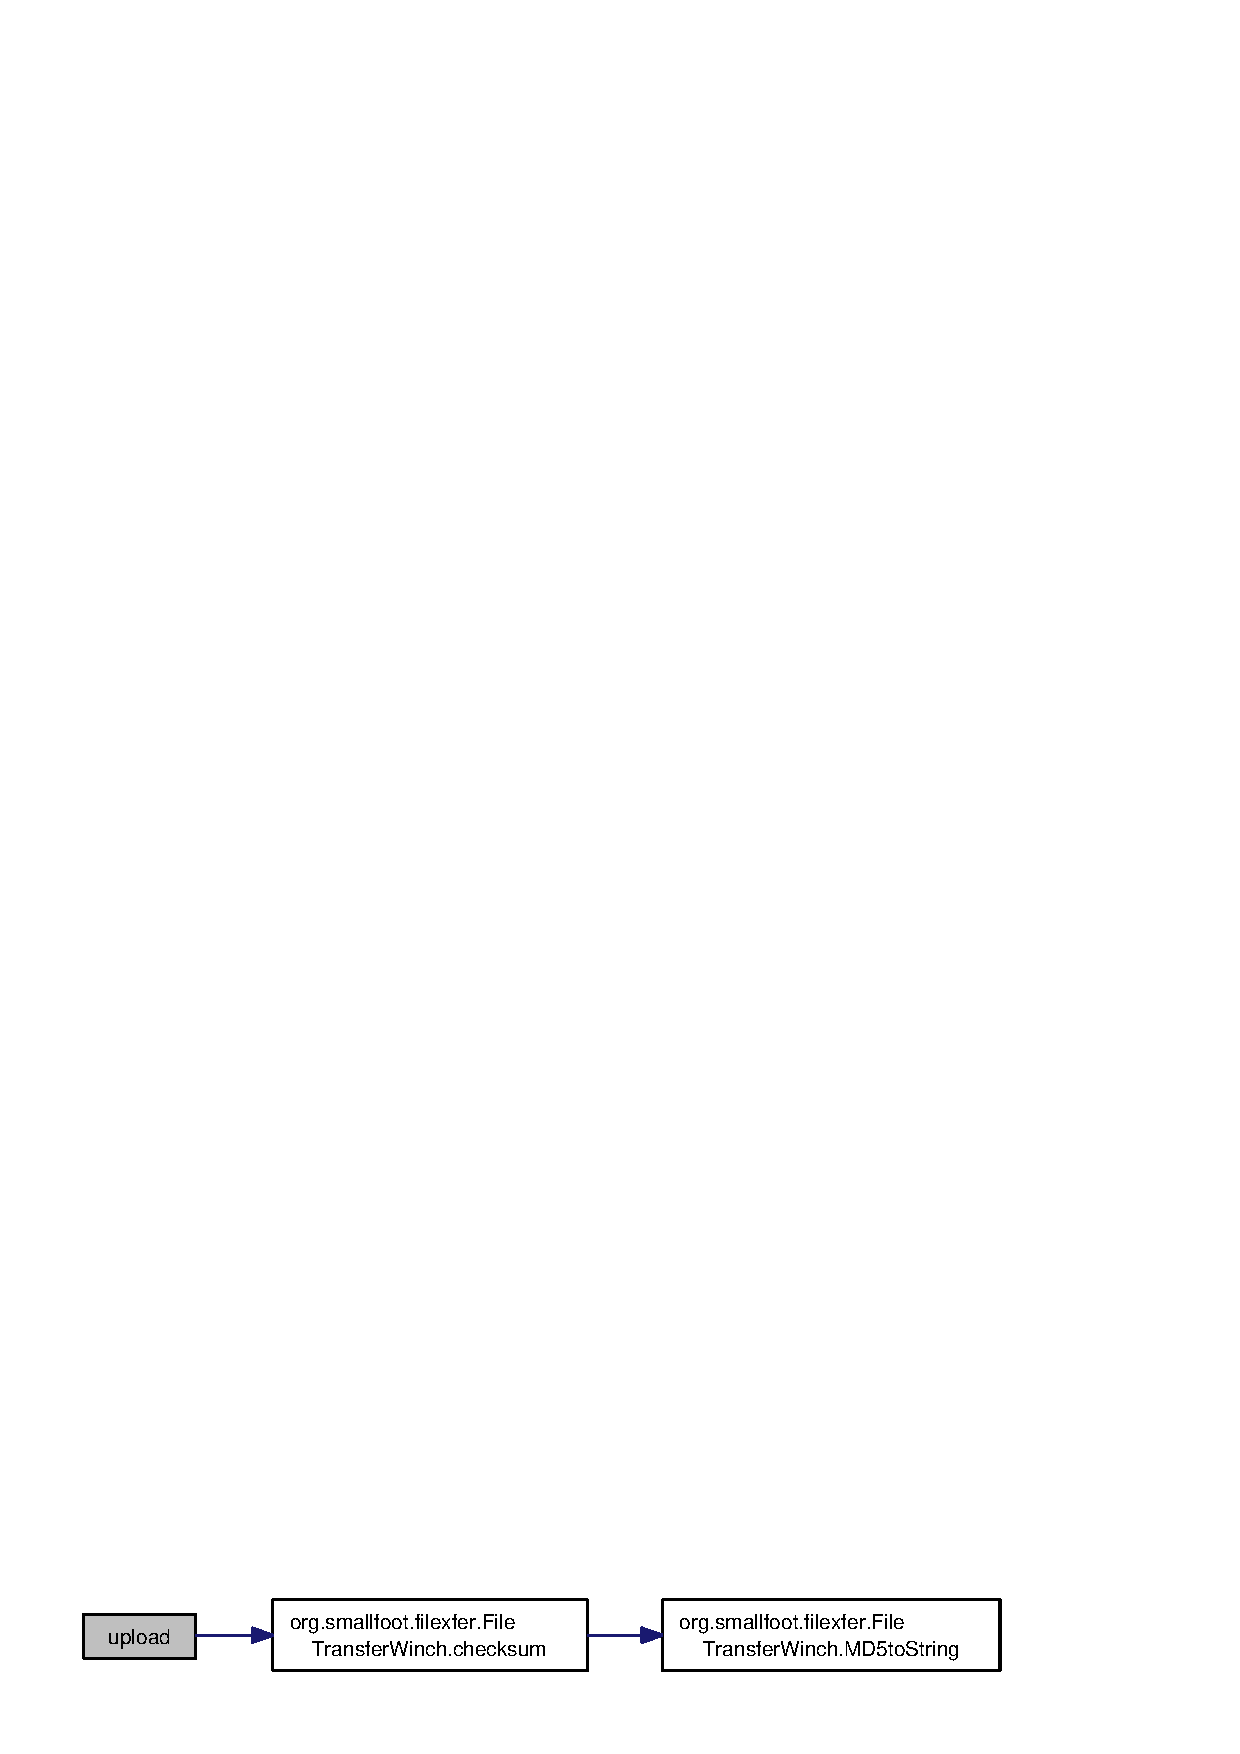
\includegraphics[width=350pt]{classorg_1_1smallfoot_1_1filexfer_1_1ApacheCommonsNetSFTP_afa3dfccec4b989cafc56103eb1ee82a6_cgraph}
\end{center}
\end{figure}




The documentation for this class was generated from the following file\+:\begin{DoxyCompactItemize}
\item 
java/Apache\+Commons\+Net\+S\+F\+T\+P.\+java\end{DoxyCompactItemize}

\section{File\+Transfer\+Winch.\+File\+Transfer\+Aborted\+Exception Class Reference}
\label{classorg_1_1smallfoot_1_1filexfer_1_1FileTransferWinch_1_1FileTransferAbortedException}\index{File\+Transfer\+Winch.\+File\+Transfer\+Aborted\+Exception@{File\+Transfer\+Winch.\+File\+Transfer\+Aborted\+Exception}}


This exception indicates that transfer was aborted; I have not yet clarified in the A\+P\+I whether this exception would take precidence over \doxyref{File\+Transfer\+Data\+Transfer\+Exception}{p.}{classorg_1_1smallfoot_1_1filexfer_1_1FileTransferWinch_1_1FileTransferDataTransferException} if both occur, or a \doxyref{File\+Transfer\+Data\+Transfer\+Exception}{p.}{classorg_1_1smallfoot_1_1filexfer_1_1FileTransferWinch_1_1FileTransferDataTransferException} causes a \doxyref{File\+Transfer\+Aborted\+Exception}{p.}{classorg_1_1smallfoot_1_1filexfer_1_1FileTransferWinch_1_1FileTransferAbortedException}.  




Inheritance diagram for File\+Transfer\+Winch.\+File\+Transfer\+Aborted\+Exception\+:\nopagebreak
\begin{figure}[H]
\begin{center}
\leavevmode
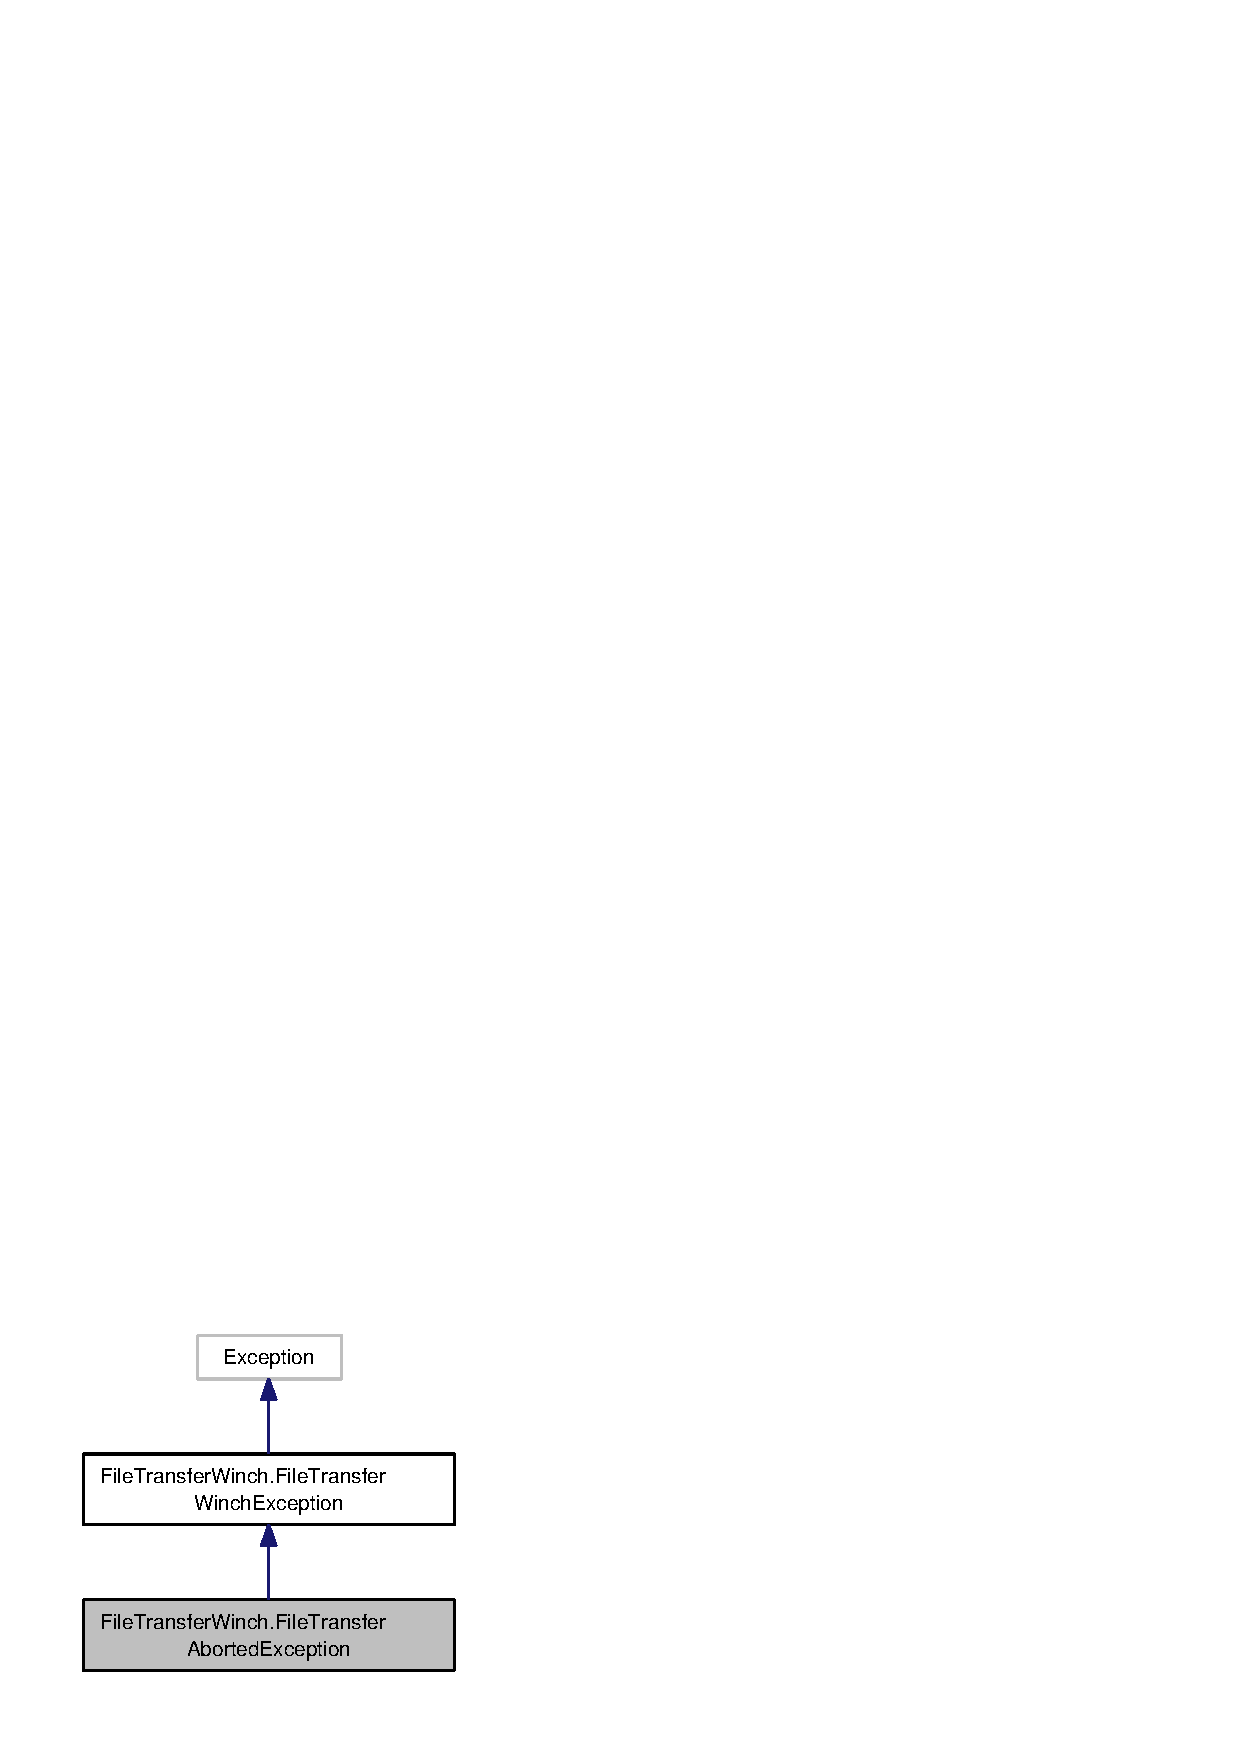
\includegraphics[width=196pt]{classorg_1_1smallfoot_1_1filexfer_1_1FileTransferWinch_1_1FileTransferAbortedException__inherit__graph}
\end{center}
\end{figure}


Collaboration diagram for File\+Transfer\+Winch.\+File\+Transfer\+Aborted\+Exception\+:\nopagebreak
\begin{figure}[H]
\begin{center}
\leavevmode
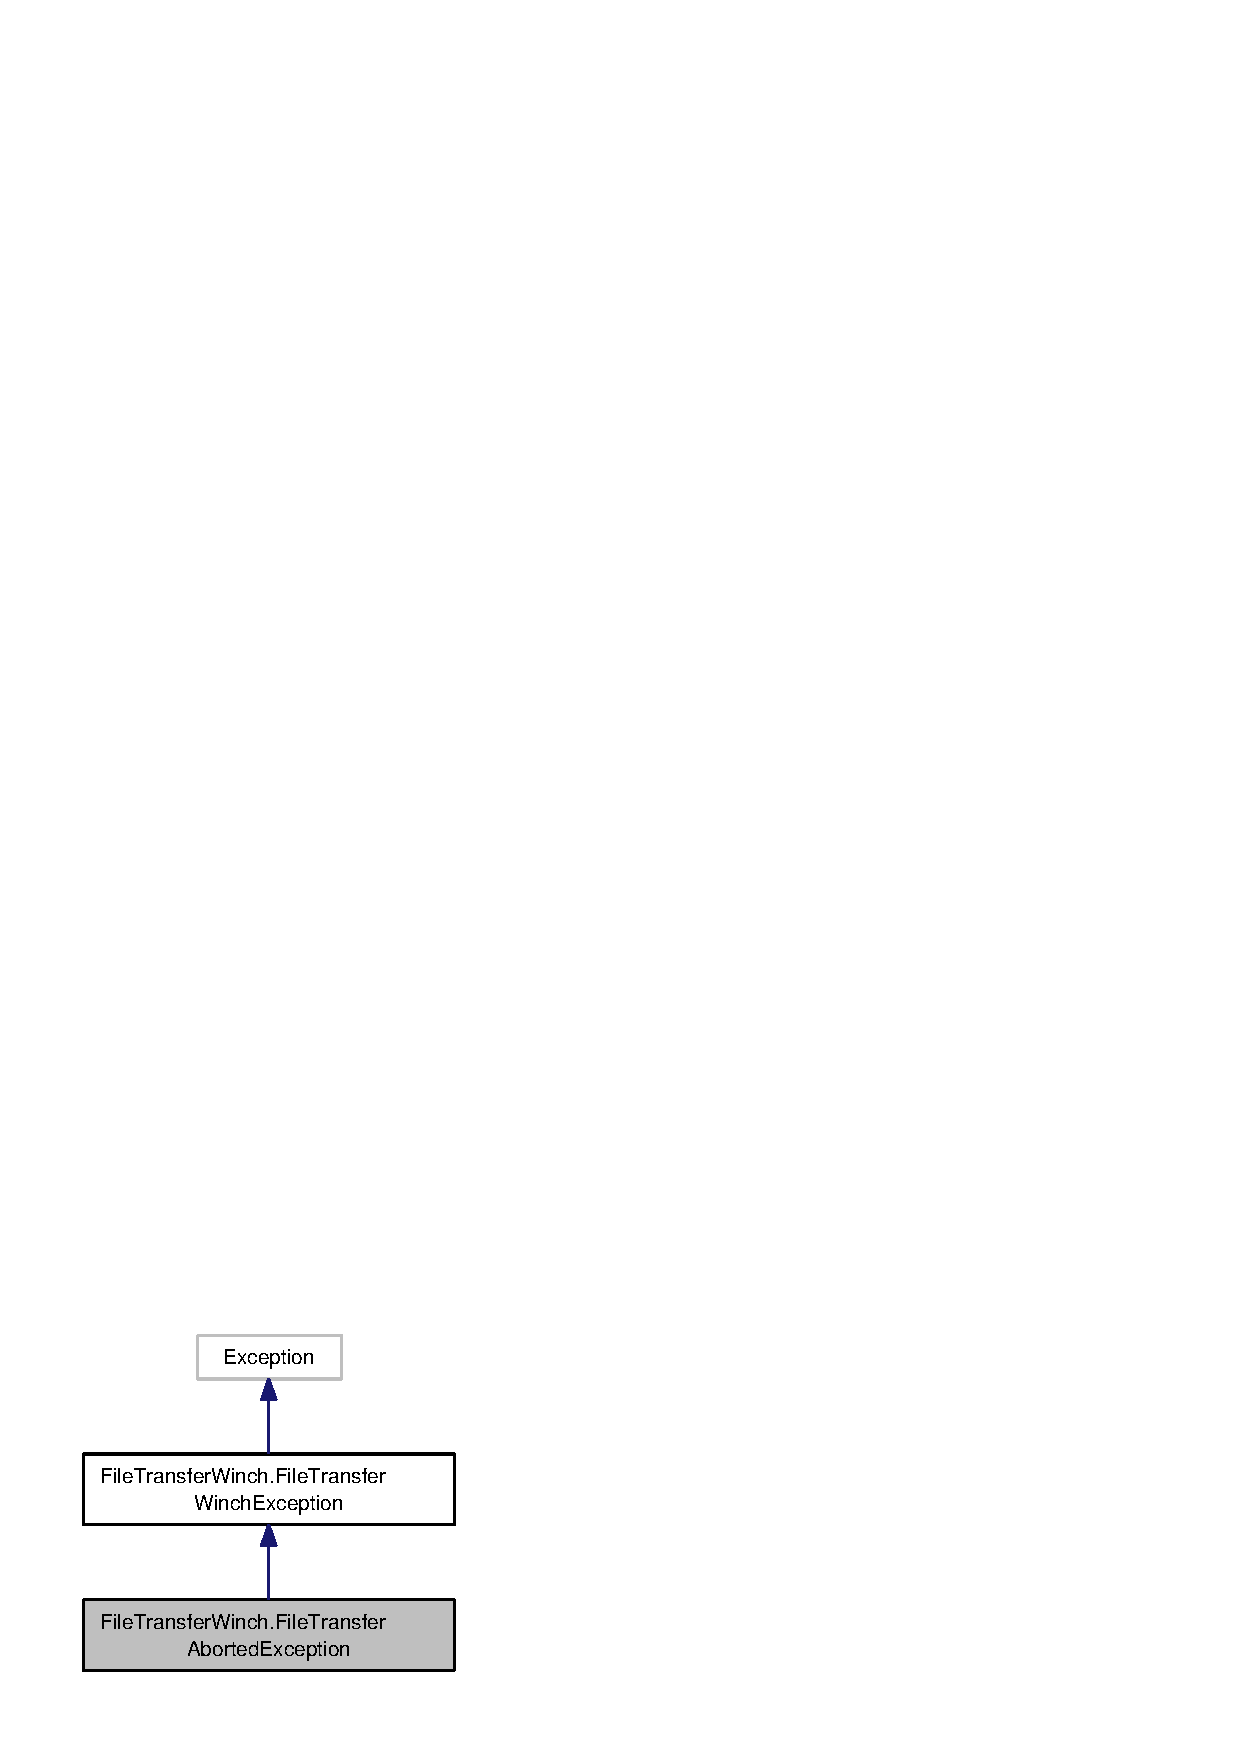
\includegraphics[width=196pt]{classorg_1_1smallfoot_1_1filexfer_1_1FileTransferWinch_1_1FileTransferAbortedException__coll__graph}
\end{center}
\end{figure}
\subsection*{Public Member Functions}
\begin{DoxyCompactItemize}
\item 
{\bfseries File\+Transfer\+Aborted\+Exception} (String s, Throwable t)\label{classorg_1_1smallfoot_1_1filexfer_1_1FileTransferWinch_1_1FileTransferAbortedException_ac659126c0b9e888dd6c0a91560e69c19}

\item 
{\bfseries File\+Transfer\+Aborted\+Exception} (Throwable t)\label{classorg_1_1smallfoot_1_1filexfer_1_1FileTransferWinch_1_1FileTransferAbortedException_a6d0ddeded5d8a06a0a6e8dc5428642a9}

\item 
{\bfseries File\+Transfer\+Aborted\+Exception} (String s)\label{classorg_1_1smallfoot_1_1filexfer_1_1FileTransferWinch_1_1FileTransferAbortedException_a5d7f46551725ecdab4fbfd1c8caae3c6}

\end{DoxyCompactItemize}


\subsection{Detailed Description}
This exception indicates that transfer was aborted; I have not yet clarified in the A\+P\+I whether this exception would take precidence over \doxyref{File\+Transfer\+Data\+Transfer\+Exception}{p.}{classorg_1_1smallfoot_1_1filexfer_1_1FileTransferWinch_1_1FileTransferDataTransferException} if both occur, or a \doxyref{File\+Transfer\+Data\+Transfer\+Exception}{p.}{classorg_1_1smallfoot_1_1filexfer_1_1FileTransferWinch_1_1FileTransferDataTransferException} causes a \doxyref{File\+Transfer\+Aborted\+Exception}{p.}{classorg_1_1smallfoot_1_1filexfer_1_1FileTransferWinch_1_1FileTransferAbortedException}. 

Definition at line 122 of file File\+Transfer\+Winch.\+java.



The documentation for this class was generated from the following file\+:\begin{DoxyCompactItemize}
\item 
java/File\+Transfer\+Winch.\+java\end{DoxyCompactItemize}

\section{File\-Transfer\-Winch.\-File\-Transfer\-Checksum\-Mismatch\-Exception Class Reference}
\label{classorg_1_1smallfoot_1_1filexfer_1_1FileTransferWinch_1_1FileTransferChecksumMismatchException}\index{File\-Transfer\-Winch.\-File\-Transfer\-Checksum\-Mismatch\-Exception@{File\-Transfer\-Winch.\-File\-Transfer\-Checksum\-Mismatch\-Exception}}


This exception alerts to the specific Data Transfer issuesuch that the receiver's checksum confirmation did not match the sender ...  




Inheritance diagram for File\-Transfer\-Winch.\-File\-Transfer\-Checksum\-Mismatch\-Exception\-:\nopagebreak
\begin{figure}[H]
\begin{center}
\leavevmode
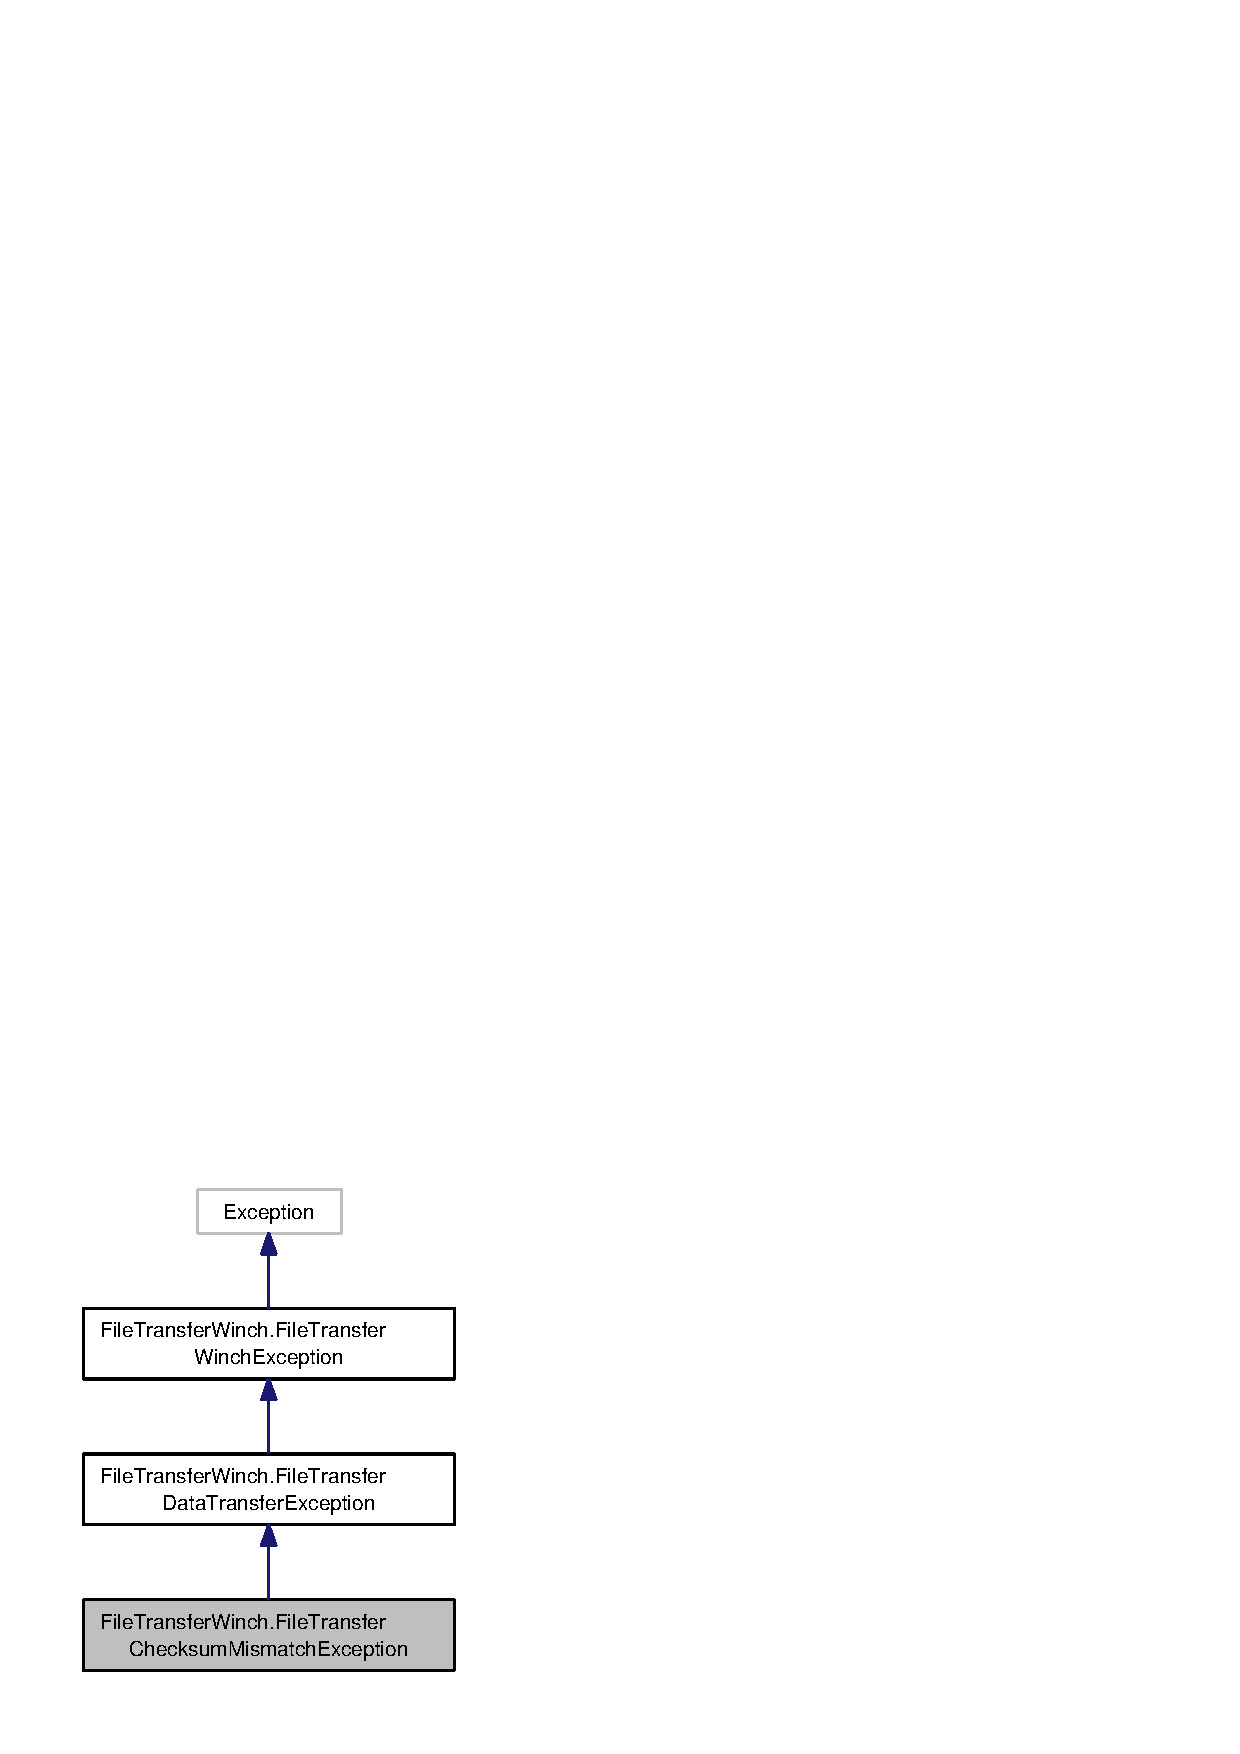
\includegraphics[width=222pt]{classorg_1_1smallfoot_1_1filexfer_1_1FileTransferWinch_1_1FileTransferChecksumMismatchException__inherit__graph}
\end{center}
\end{figure}


Collaboration diagram for File\-Transfer\-Winch.\-File\-Transfer\-Checksum\-Mismatch\-Exception\-:\nopagebreak
\begin{figure}[H]
\begin{center}
\leavevmode
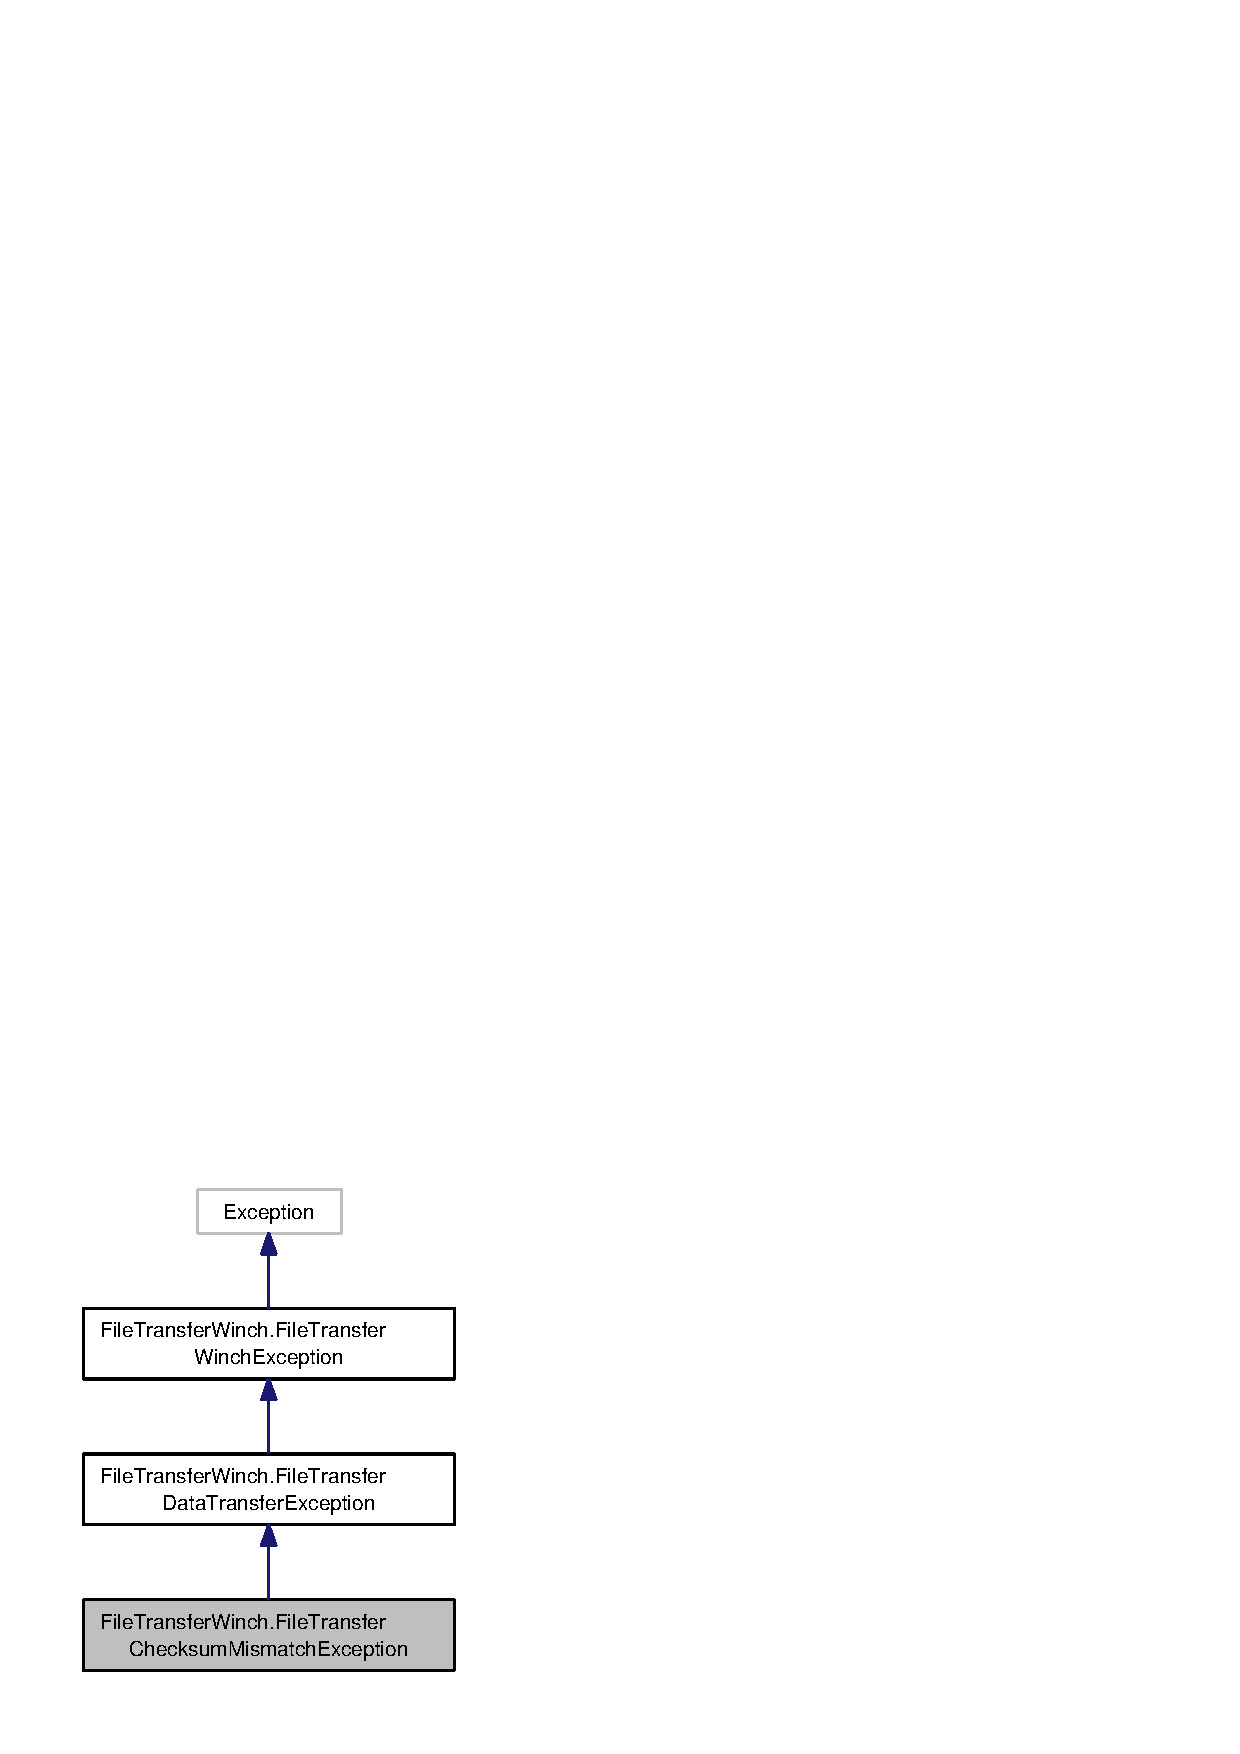
\includegraphics[width=222pt]{classorg_1_1smallfoot_1_1filexfer_1_1FileTransferWinch_1_1FileTransferChecksumMismatchException__coll__graph}
\end{center}
\end{figure}
\subsection*{Public Member Functions}
\begin{DoxyCompactItemize}
\item 
{\bfseries File\-Transfer\-Checksum\-Mismatch\-Exception} (String s, Throwable t)\label{classorg_1_1smallfoot_1_1filexfer_1_1FileTransferWinch_1_1FileTransferChecksumMismatchException_a68f39ff221119291117ba025fbaf6b48}

\item 
{\bfseries File\-Transfer\-Checksum\-Mismatch\-Exception} (Throwable t)\label{classorg_1_1smallfoot_1_1filexfer_1_1FileTransferWinch_1_1FileTransferChecksumMismatchException_a8c8c31fd8e685938b30b756523b56f09}

\item 
{\bfseries File\-Transfer\-Checksum\-Mismatch\-Exception} (String s)\label{classorg_1_1smallfoot_1_1filexfer_1_1FileTransferWinch_1_1FileTransferChecksumMismatchException_ae18c6b90199429c6b6b4dadd5f3f58ab}

\end{DoxyCompactItemize}


\subsection{Detailed Description}
This exception alerts to the specific Data Transfer issuesuch that the receiver's checksum confirmation did not match the sender ... 



Definition at line 104 of file File\-Transfer\-Winch.\-java.



The documentation for this class was generated from the following file\-:\begin{DoxyCompactItemize}
\item 
java/File\-Transfer\-Winch.\-java\end{DoxyCompactItemize}

\section{File\+Transfer\+Winch.\+File\+Transfer\+Data\+Transfer\+Exception Class Reference}
\label{classorg_1_1smallfoot_1_1filexfer_1_1FileTransferWinch_1_1FileTransferDataTransferException}\index{File\+Transfer\+Winch.\+File\+Transfer\+Data\+Transfer\+Exception@{File\+Transfer\+Winch.\+File\+Transfer\+Data\+Transfer\+Exception}}


This exception alerts to issues during transfer of data\+: connection lost, etc ...  




Inheritance diagram for File\+Transfer\+Winch.\+File\+Transfer\+Data\+Transfer\+Exception\+:\nopagebreak
\begin{figure}[H]
\begin{center}
\leavevmode
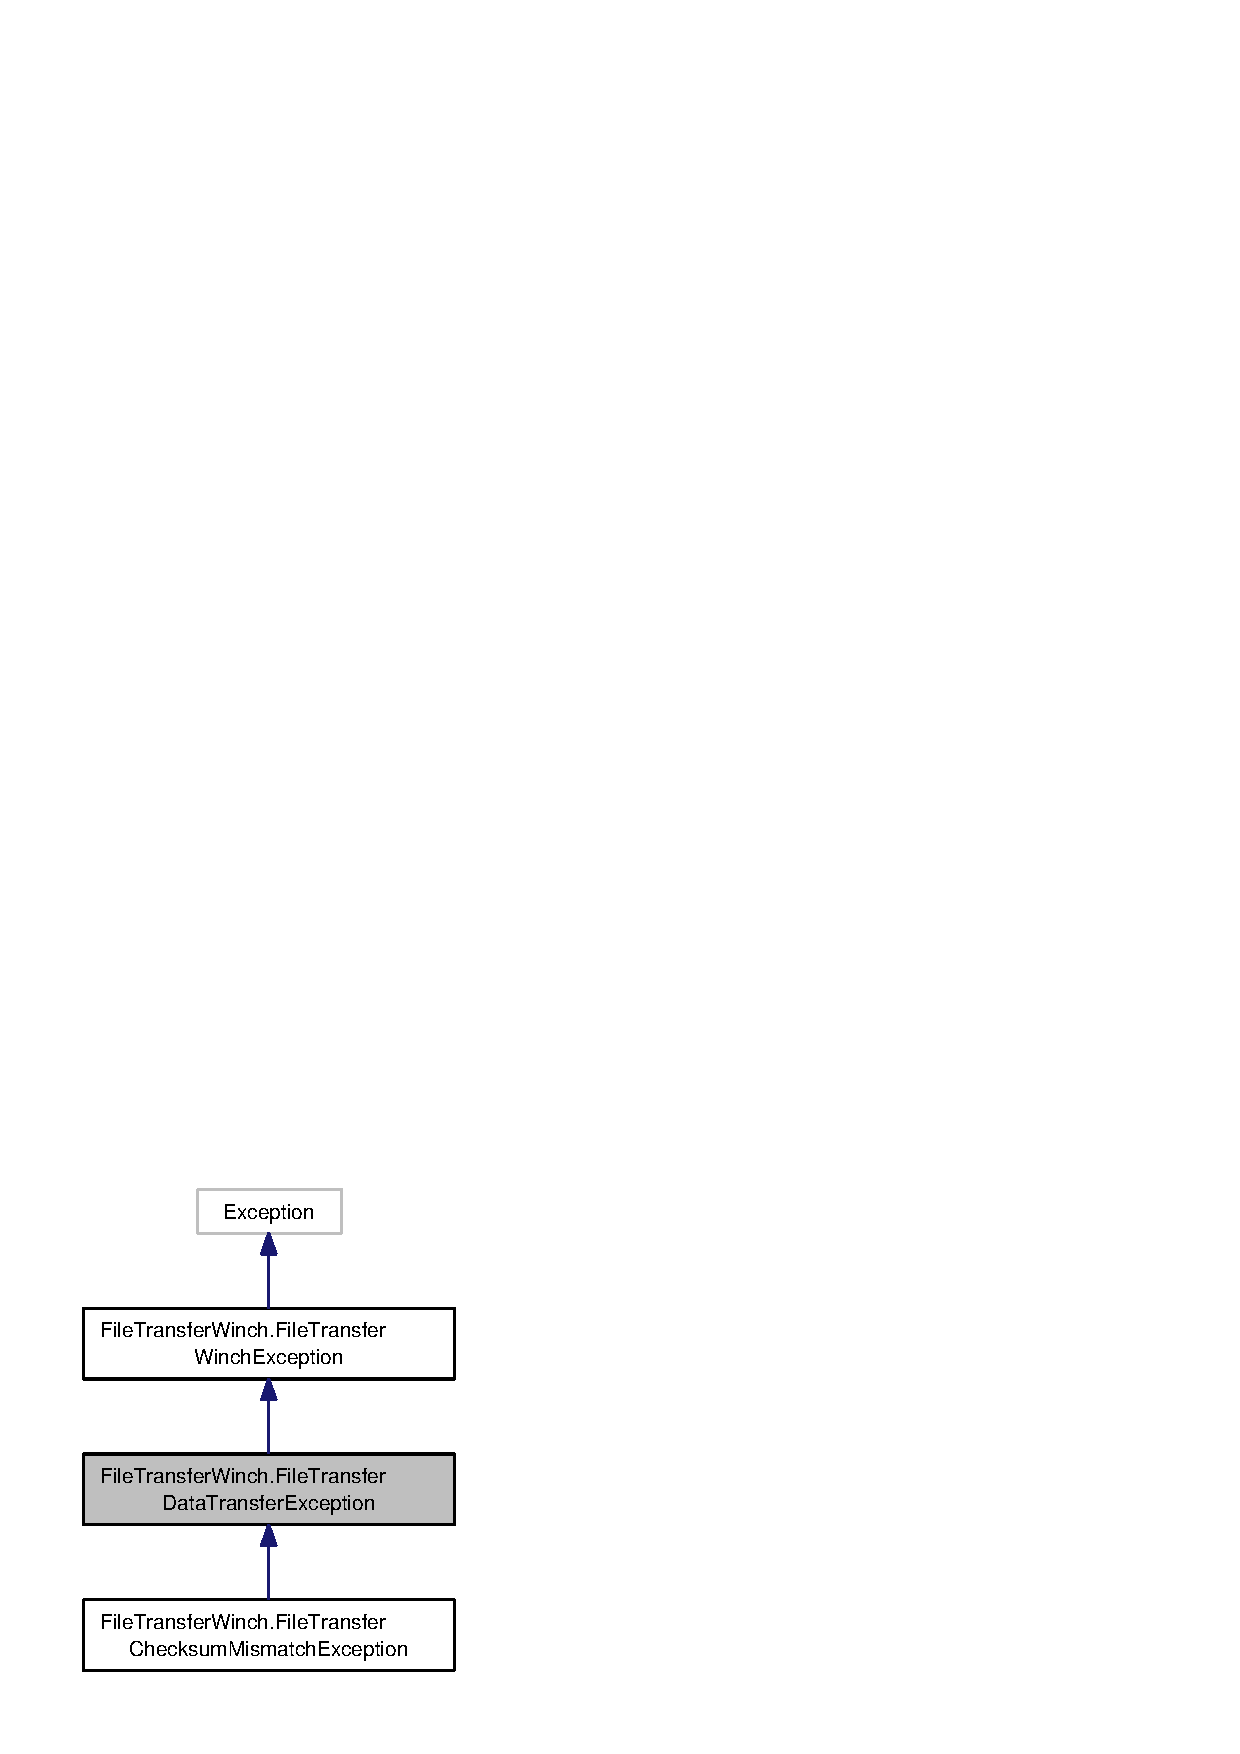
\includegraphics[width=196pt]{classorg_1_1smallfoot_1_1filexfer_1_1FileTransferWinch_1_1FileTransferDataTransferException__inherit__graph}
\end{center}
\end{figure}


Collaboration diagram for File\+Transfer\+Winch.\+File\+Transfer\+Data\+Transfer\+Exception\+:\nopagebreak
\begin{figure}[H]
\begin{center}
\leavevmode
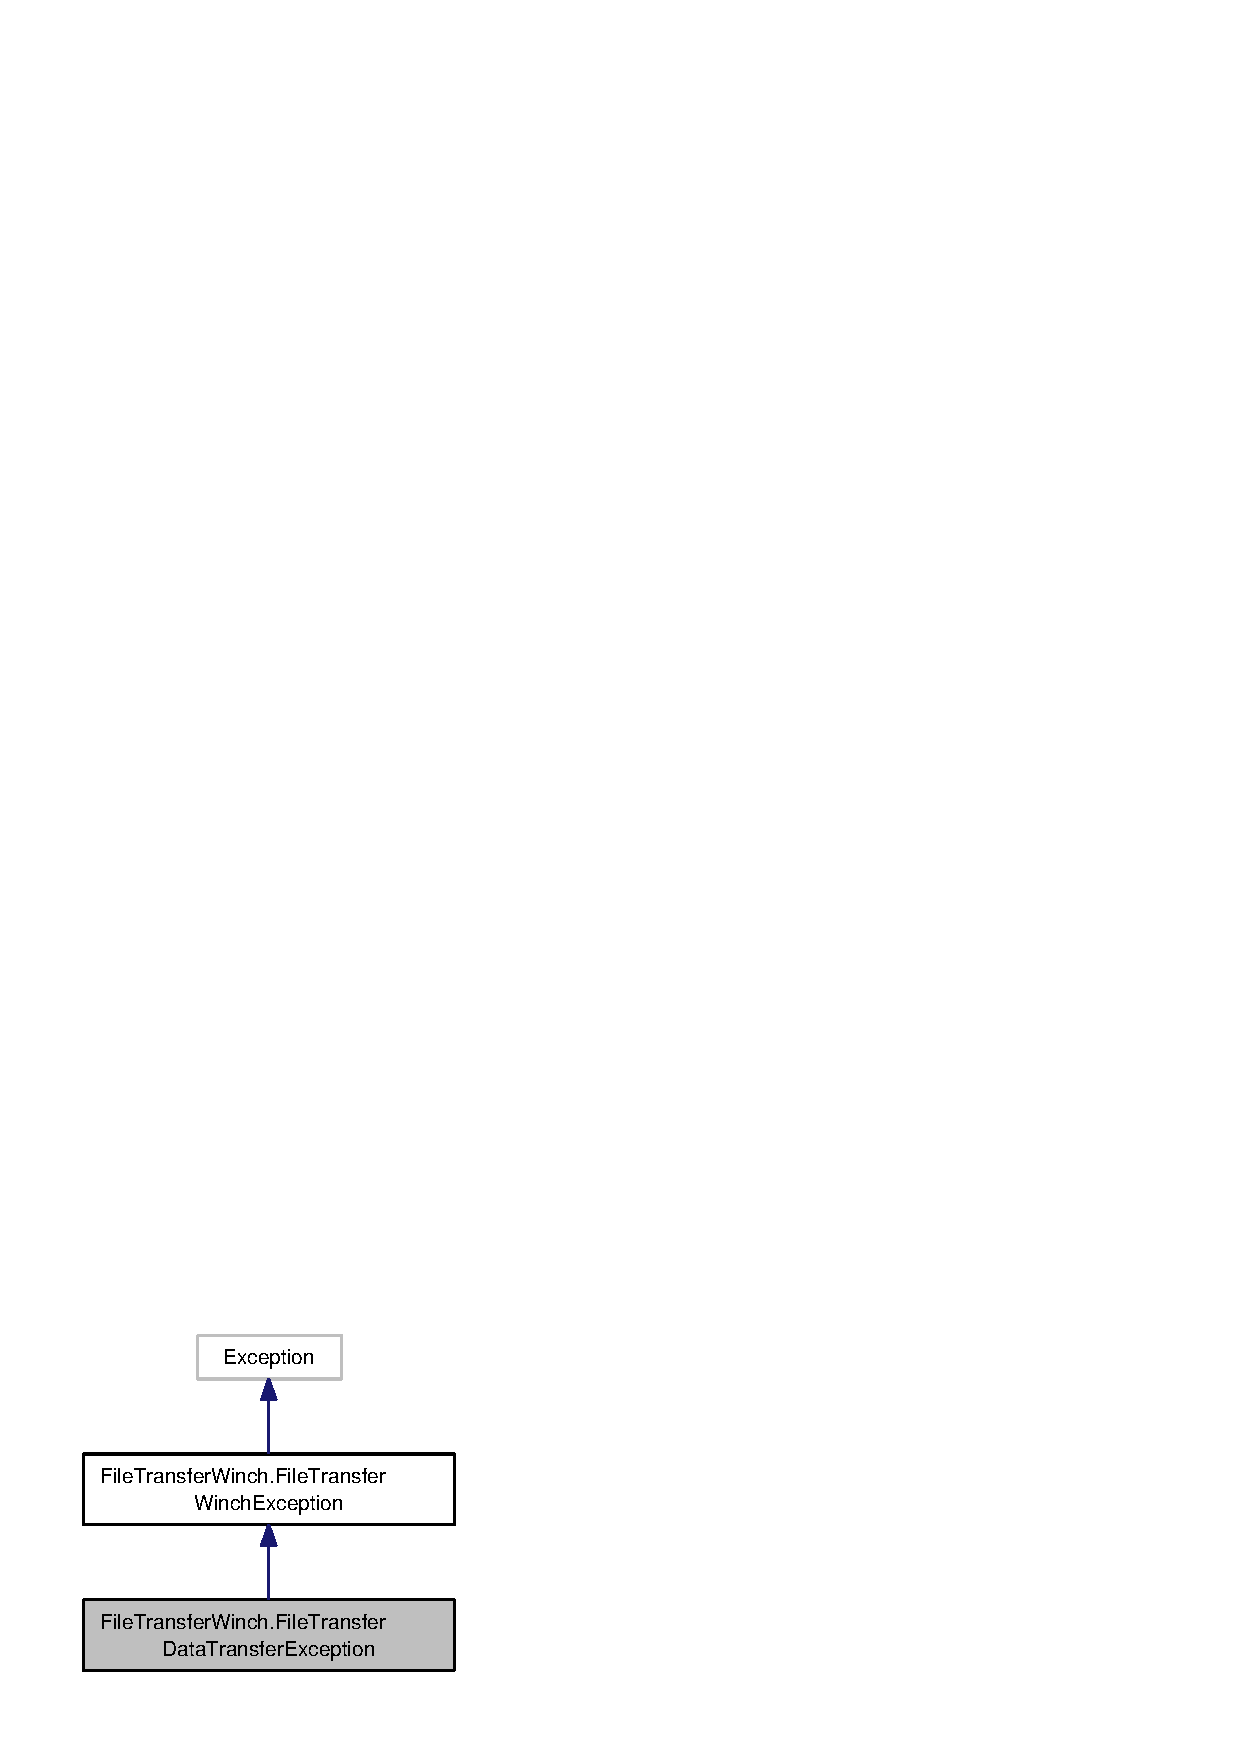
\includegraphics[width=196pt]{classorg_1_1smallfoot_1_1filexfer_1_1FileTransferWinch_1_1FileTransferDataTransferException__coll__graph}
\end{center}
\end{figure}
\subsection*{Public Member Functions}
\begin{DoxyCompactItemize}
\item 
{\bfseries File\+Transfer\+Data\+Transfer\+Exception} (String s, Throwable t)\label{classorg_1_1smallfoot_1_1filexfer_1_1FileTransferWinch_1_1FileTransferDataTransferException_a7eebb8f05696cd7cfd131b36ca392895}

\item 
{\bfseries File\+Transfer\+Data\+Transfer\+Exception} (Throwable t)\label{classorg_1_1smallfoot_1_1filexfer_1_1FileTransferWinch_1_1FileTransferDataTransferException_a730a4e8226d9a8b6cd43aa50687e854c}

\item 
{\bfseries File\+Transfer\+Data\+Transfer\+Exception} (String s)\label{classorg_1_1smallfoot_1_1filexfer_1_1FileTransferWinch_1_1FileTransferDataTransferException_a3609c8674a0be3d2ecc75870110a95ff}

\end{DoxyCompactItemize}


\subsection{Detailed Description}
This exception alerts to issues during transfer of data\+: connection lost, etc ... 



Definition at line 86 of file File\+Transfer\+Winch.\+java.



The documentation for this class was generated from the following file\+:\begin{DoxyCompactItemize}
\item 
java/File\+Transfer\+Winch.\+java\end{DoxyCompactItemize}

\section{File\+Transfer\+Winch.\+File\+Transfer\+Illegal\+F\+S\+M\+Reply\+Exception Class Reference}
\label{classorg_1_1smallfoot_1_1filexfer_1_1FileTransferWinch_1_1FileTransferIllegalFSMReplyException}\index{File\+Transfer\+Winch.\+File\+Transfer\+Illegal\+F\+S\+M\+Reply\+Exception@{File\+Transfer\+Winch.\+File\+Transfer\+Illegal\+F\+S\+M\+Reply\+Exception}}


This exception indicates that the underlying Finite State Machine received an unexpected reply, and has no next-\/state in the conversation.  




Inheritance diagram for File\+Transfer\+Winch.\+File\+Transfer\+Illegal\+F\+S\+M\+Reply\+Exception\+:\nopagebreak
\begin{figure}[H]
\begin{center}
\leavevmode
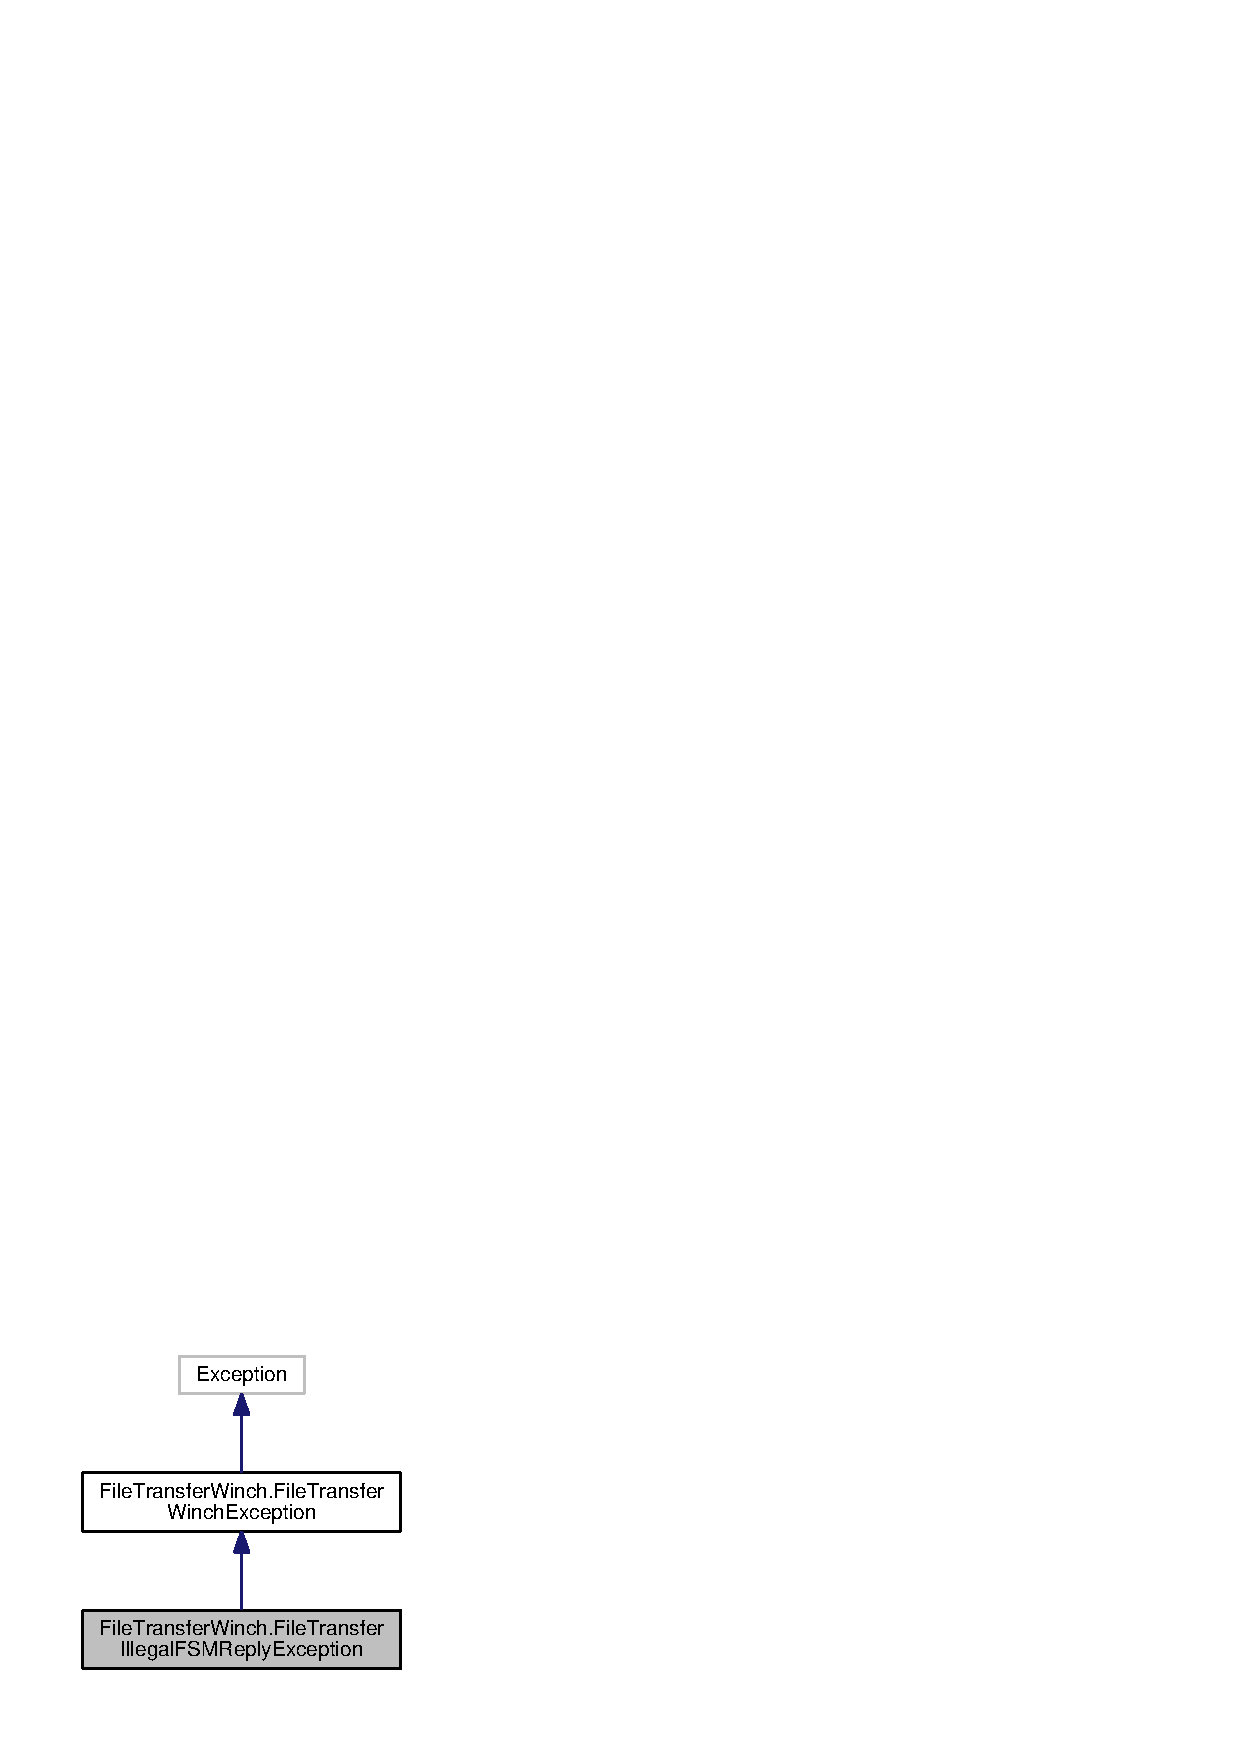
\includegraphics[width=196pt]{classorg_1_1smallfoot_1_1filexfer_1_1FileTransferWinch_1_1FileTransferIllegalFSMReplyException__inherit__graph}
\end{center}
\end{figure}


Collaboration diagram for File\+Transfer\+Winch.\+File\+Transfer\+Illegal\+F\+S\+M\+Reply\+Exception\+:\nopagebreak
\begin{figure}[H]
\begin{center}
\leavevmode
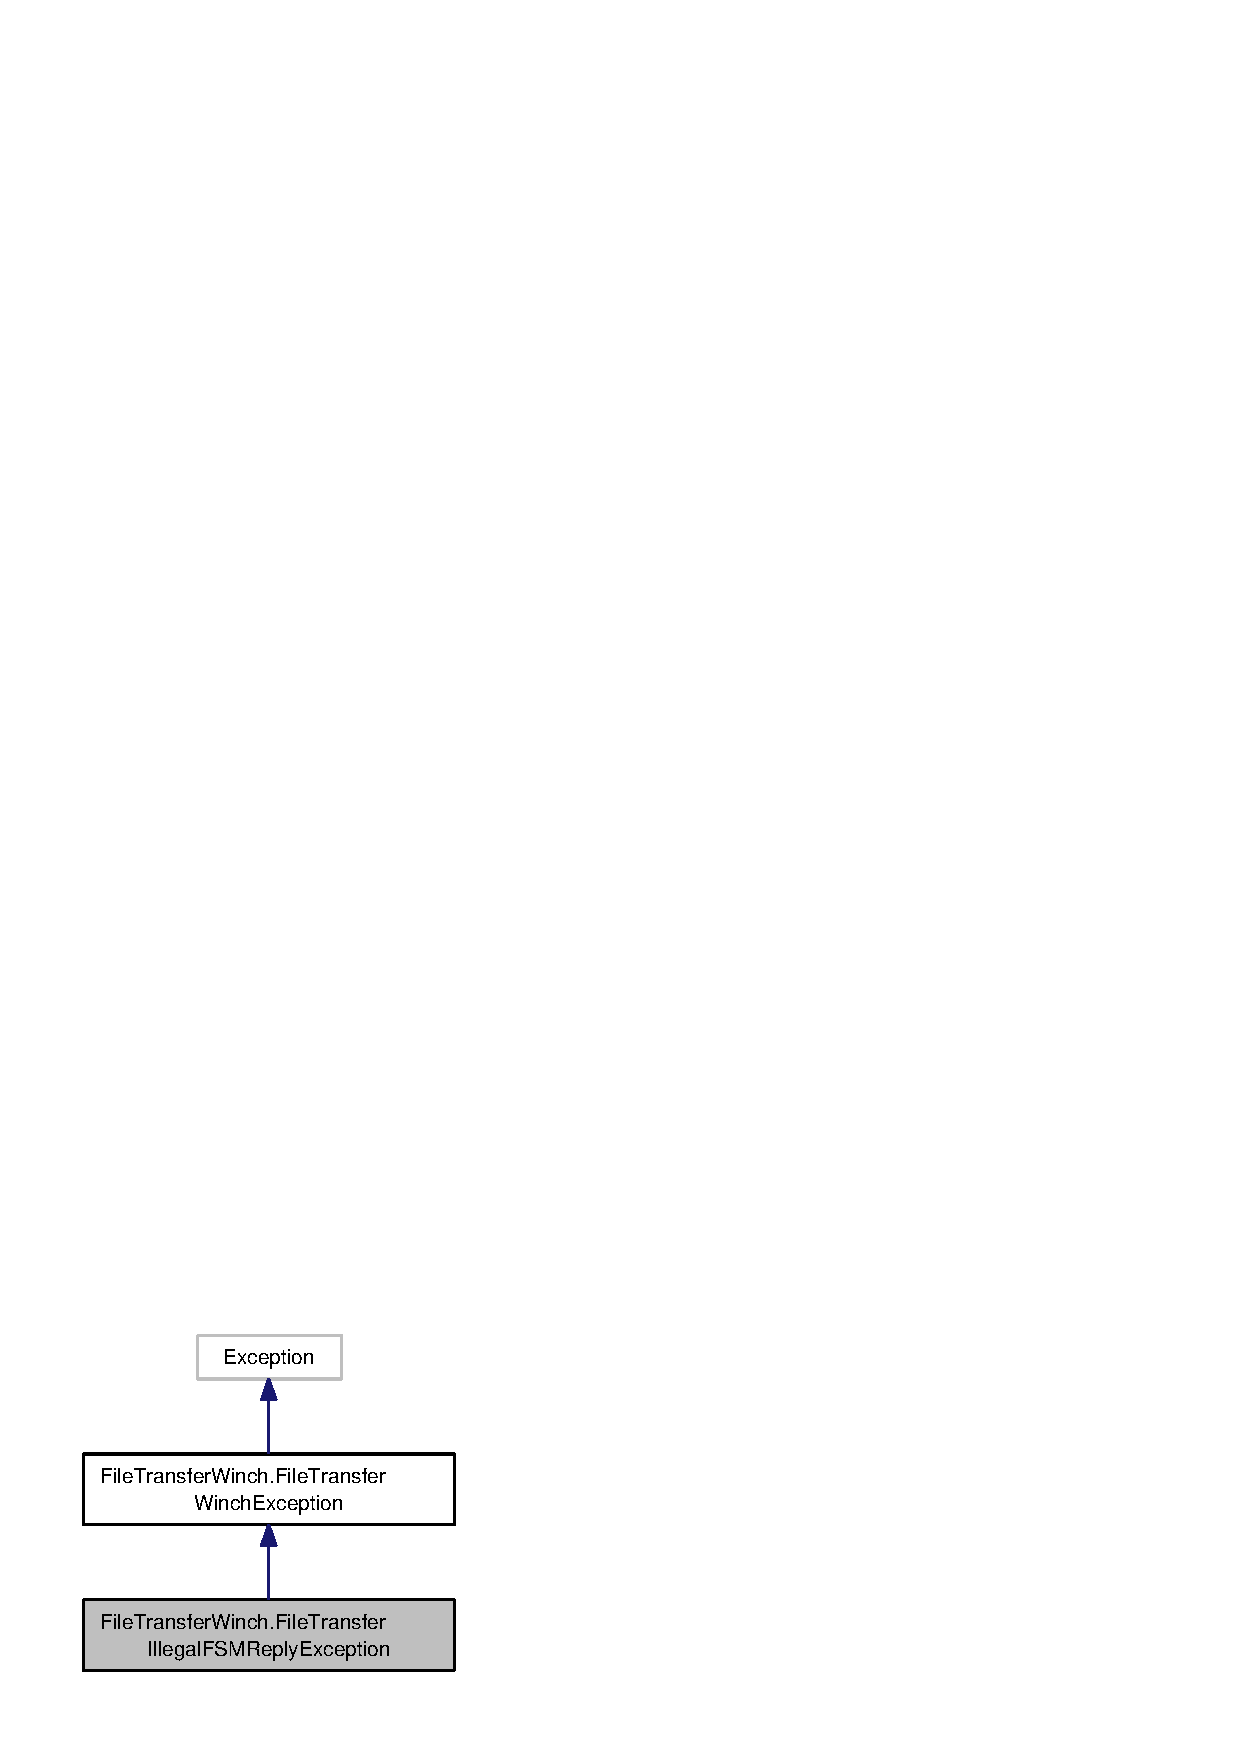
\includegraphics[width=196pt]{classorg_1_1smallfoot_1_1filexfer_1_1FileTransferWinch_1_1FileTransferIllegalFSMReplyException__coll__graph}
\end{center}
\end{figure}
\subsection*{Public Member Functions}
\begin{DoxyCompactItemize}
\item 
{\bfseries File\+Transfer\+Illegal\+F\+S\+M\+Reply\+Exception} (String s, Throwable t)\label{classorg_1_1smallfoot_1_1filexfer_1_1FileTransferWinch_1_1FileTransferIllegalFSMReplyException_ad27ca86ec85b2c39c339bdaf0eee3560}

\item 
{\bfseries File\+Transfer\+Illegal\+F\+S\+M\+Reply\+Exception} (Throwable t)\label{classorg_1_1smallfoot_1_1filexfer_1_1FileTransferWinch_1_1FileTransferIllegalFSMReplyException_a4e8ffe04c5de02a5750e97613ef40af8}

\item 
{\bfseries File\+Transfer\+Illegal\+F\+S\+M\+Reply\+Exception} (String s)\label{classorg_1_1smallfoot_1_1filexfer_1_1FileTransferWinch_1_1FileTransferIllegalFSMReplyException_a2e552ceb66966a3493c3c47227d5ba6c}

\end{DoxyCompactItemize}


\subsection{Detailed Description}
This exception indicates that the underlying Finite State Machine received an unexpected reply, and has no next-\/state in the conversation. 

Basically\+: \char`\"{}the other side said something and I didn't know what to do \char`\"{}. 

Definition at line 68 of file File\+Transfer\+Winch.\+java.



The documentation for this class was generated from the following file\+:\begin{DoxyCompactItemize}
\item 
java/File\+Transfer\+Winch.\+java\end{DoxyCompactItemize}

\section{File\+Transfer\+Winch Class Reference}
\label{classorg_1_1smallfoot_1_1filexfer_1_1FileTransferWinch}\index{File\+Transfer\+Winch@{File\+Transfer\+Winch}}


Inheritance diagram for File\+Transfer\+Winch\+:\nopagebreak
\begin{figure}[H]
\begin{center}
\leavevmode
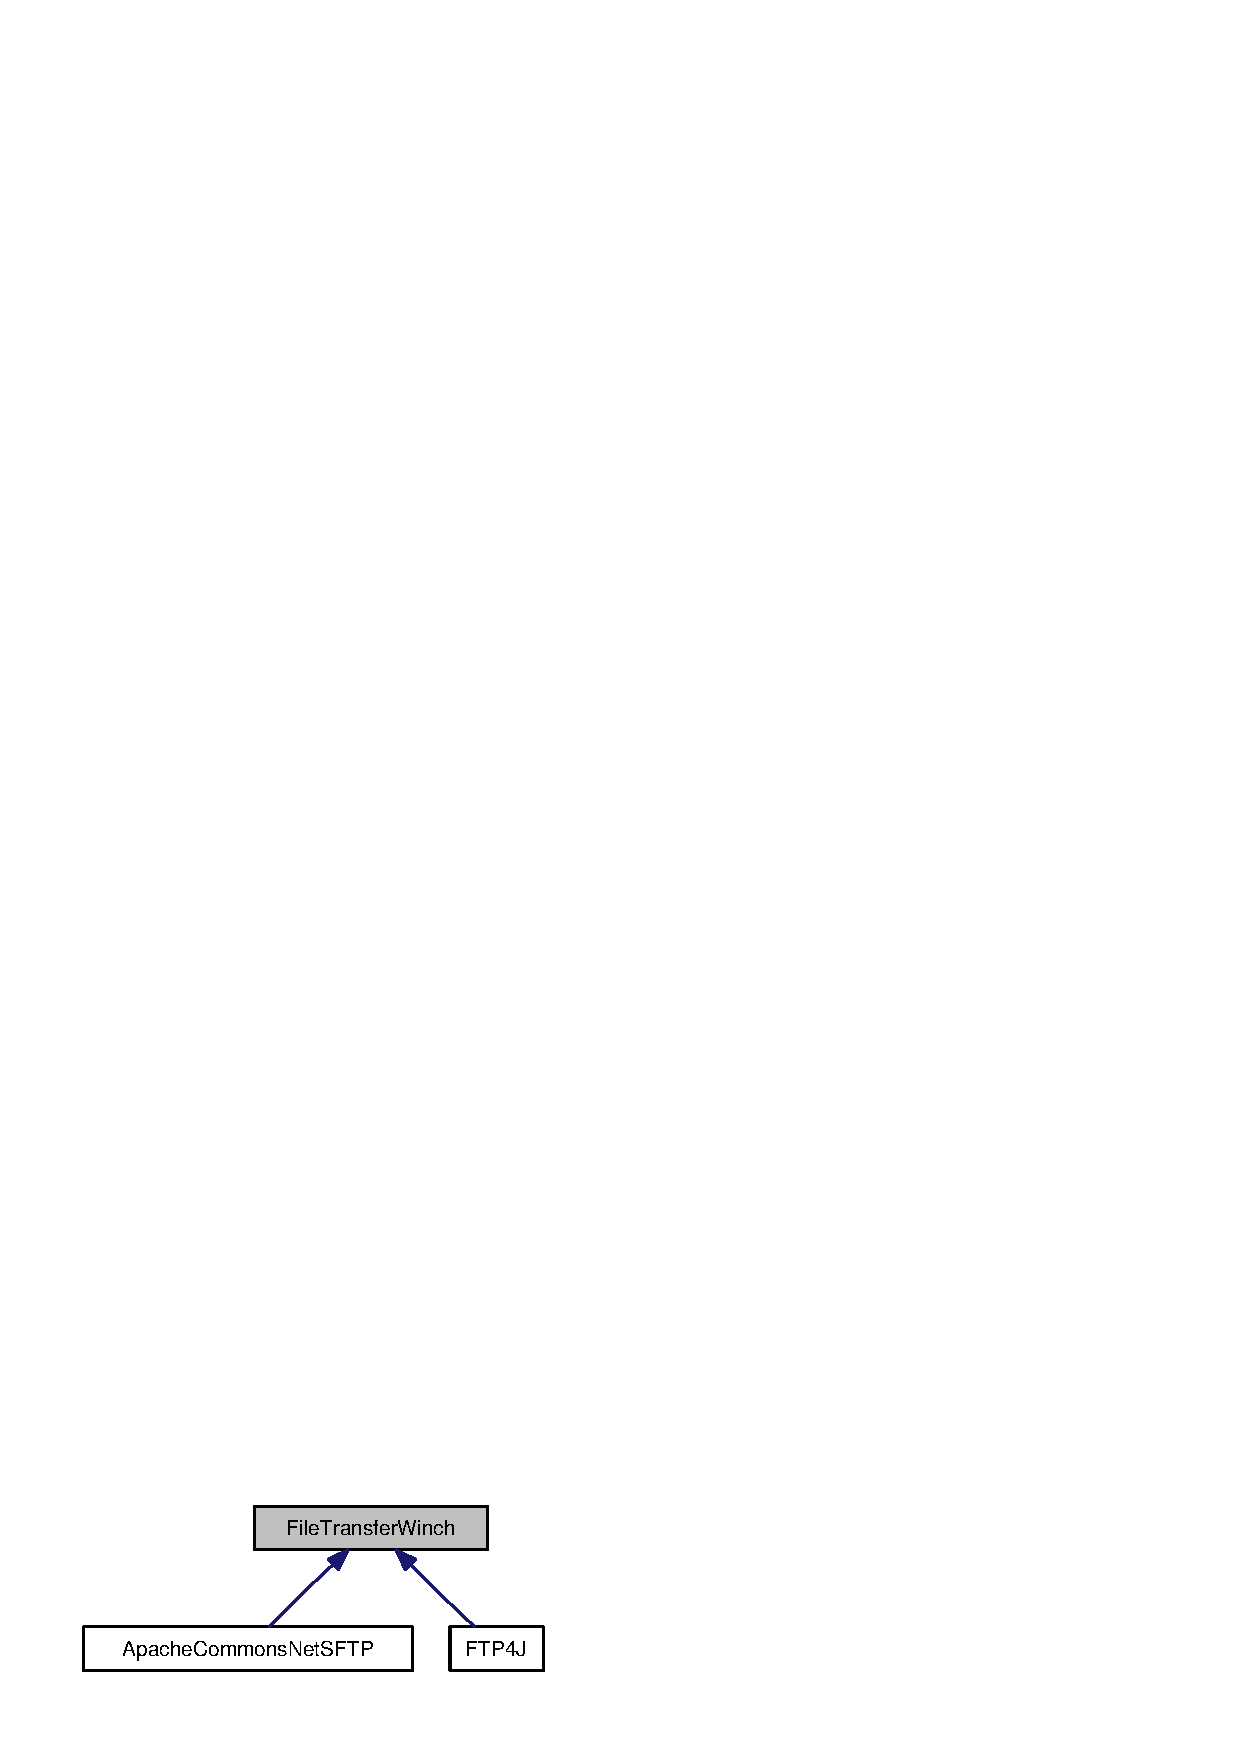
\includegraphics[width=264pt]{classorg_1_1smallfoot_1_1filexfer_1_1FileTransferWinch__inherit__graph}
\end{center}
\end{figure}
\subsection*{Data Structures}
\begin{DoxyCompactItemize}
\item 
class {\bf File\+Transfer\+Aborted\+Exception}
\begin{DoxyCompactList}\small\item\em This exception indicates that transfer was aborted; I have not yet clarified in the A\+P\+I whether this exception would take precidence over \doxyref{File\+Transfer\+Data\+Transfer\+Exception}{p.}{classorg_1_1smallfoot_1_1filexfer_1_1FileTransferWinch_1_1FileTransferDataTransferException} if both occur, or a \doxyref{File\+Transfer\+Data\+Transfer\+Exception}{p.}{classorg_1_1smallfoot_1_1filexfer_1_1FileTransferWinch_1_1FileTransferDataTransferException} causes a \doxyref{File\+Transfer\+Aborted\+Exception}{p.}{classorg_1_1smallfoot_1_1filexfer_1_1FileTransferWinch_1_1FileTransferAbortedException}. \end{DoxyCompactList}\item 
class {\bf File\+Transfer\+Checksum\+Mismatch\+Exception}
\begin{DoxyCompactList}\small\item\em This exception alerts to the specific Data Transfer issuesuch that the receiver's checksum confirmation did not match the sender ... \end{DoxyCompactList}\item 
class {\bf File\+Transfer\+Data\+Transfer\+Exception}
\begin{DoxyCompactList}\small\item\em This exception alerts to issues during transfer of data\+: connection lost, etc ... \end{DoxyCompactList}\item 
class {\bf File\+Transfer\+Illegal\+F\+S\+M\+Reply\+Exception}
\begin{DoxyCompactList}\small\item\em This exception indicates that the underlying Finite State Machine received an unexpected reply, and has no next-\/state in the conversation. \end{DoxyCompactList}\item 
class {\bf File\+Transfer\+Winch\+Exception}
\begin{DoxyCompactList}\small\item\em A base collector exception\+: \char`\"{}there was some exception in the File\+Transfer\+Winch class\char`\"{}; typically, more meaning and/or usefulness is reached by catching specific subclasses of this exception. \end{DoxyCompactList}\end{DoxyCompactItemize}
\subsection*{Public Member Functions}
\begin{DoxyCompactItemize}
\item 
String {\bfseries get\+Host} ()\label{classorg_1_1smallfoot_1_1filexfer_1_1FileTransferWinch_a976c78af5cffbf292c6a1ad4f8f5f352}

\item 
String {\bfseries get\+Pass} ()\label{classorg_1_1smallfoot_1_1filexfer_1_1FileTransferWinch_a6cba30c67b9a7c8d4750e7e3108961c6}

\item 
String {\bfseries get\+Path} ()\label{classorg_1_1smallfoot_1_1filexfer_1_1FileTransferWinch_a6779d0f135fcec6c7f8a8ee49d7af165}

\item 
String {\bfseries get\+User} ()\label{classorg_1_1smallfoot_1_1filexfer_1_1FileTransferWinch_af8214ba89d8ad71194a2d69bea5cb808}

\item 
String {\bfseries name} ()\label{classorg_1_1smallfoot_1_1filexfer_1_1FileTransferWinch_afa2149aced9d90555f788dfc81c23d15}

\item 
abstract boolean {\bf upload} (File file, Vector$<$ String $>$ upload\+Notify)  throws File\+Transfer\+Winch\+Exception
\begin{DoxyCompactList}\small\item\em upload a file using this \doxyref{File\+Transfer\+Winch}{p.}{classorg_1_1smallfoot_1_1filexfer_1_1FileTransferWinch}; errors in upload are handled via Exceptions \end{DoxyCompactList}\item 
boolean {\bf upload} (String file, Vector$<$ String $>$ upload\+Notify)  throws File\+Transfer\+Winch\+Exception     
\begin{DoxyCompactList}\small\item\em upload a file using this \doxyref{File\+Transfer\+Winch}{p.}{classorg_1_1smallfoot_1_1filexfer_1_1FileTransferWinch}; errors in upload are handled via Exceptions \end{DoxyCompactList}\end{DoxyCompactItemize}
\subsection*{Static Public Member Functions}
\begin{DoxyCompactItemize}
\item 
static String {\bf checksum} (File file)  throws java.\+security.\+No\+Such\+Algorithm\+Exception, java.\+io.\+File\+Not\+Found\+Exception, java.\+io.\+I\+O\+Exception     
\begin{DoxyCompactList}\small\item\em Calculate an M\+D5 checksum. \end{DoxyCompactList}\item 
static String {\bf checksum} (String file)  throws java.\+security.\+No\+Such\+Algorithm\+Exception, java.\+io.\+File\+Not\+Found\+Exception, java.\+io.\+I\+O\+Exception     
\begin{DoxyCompactList}\small\item\em Calculate an M\+D5 checksum. \end{DoxyCompactList}\item 
static String[$\,$] {\bf examples} (java.\+net.\+U\+R\+L url)
\begin{DoxyCompactList}\small\item\em list one or more example U\+R\+Ls showing the available upload/download protocols \end{DoxyCompactList}\item 
static boolean {\bfseries handles} (java.\+net.\+U\+R\+L u)\label{classorg_1_1smallfoot_1_1filexfer_1_1FileTransferWinch_a4ef8d35ab128080eb511f7e26cd7ab7b}

\item 
static String {\bf M\+D5to\+String} (byte[$\,$] digest)
\begin{DoxyCompactList}\small\item\em convert a M\+D5 digest to a printable string. \end{DoxyCompactList}\end{DoxyCompactItemize}
\subsection*{Protected Attributes}
\begin{DoxyCompactItemize}
\item 
java.\+net.\+U\+R\+L {\bfseries url} = null\label{classorg_1_1smallfoot_1_1filexfer_1_1FileTransferWinch_a7ed35f0a10205492ddcfa6dc98f7abc4}

\end{DoxyCompactItemize}


\subsection{Detailed Description}


Definition at line 6 of file File\+Transfer\+Winch.\+java.



\subsection{Member Function Documentation}
\index{org\+::smallfoot\+::filexfer\+::\+File\+Transfer\+Winch@{org\+::smallfoot\+::filexfer\+::\+File\+Transfer\+Winch}!checksum@{checksum}}
\index{checksum@{checksum}!org\+::smallfoot\+::filexfer\+::\+File\+Transfer\+Winch@{org\+::smallfoot\+::filexfer\+::\+File\+Transfer\+Winch}}
\subsubsection[{checksum}]{\setlength{\rightskip}{0pt plus 5cm}static String checksum (
\begin{DoxyParamCaption}
\item[{File}]{file}
\end{DoxyParamCaption}
) throws java.\+security.\+No\+Such\+Algorithm\+Exception, java.\+io.\+File\+Not\+Found\+Exception, java.\+io.\+I\+O\+Exception\hspace{0.3cm}{\ttfamily [inline]}, {\ttfamily [static]}}\label{classorg_1_1smallfoot_1_1filexfer_1_1FileTransferWinch_affa1c48a18997a5ea5458d162d659c63}


Calculate an M\+D5 checksum. 

In converting this file from V\+I\+Field\+Tool code, the checksum stuff was already here, so my logic was \char`\"{}why make a user search for checksumming tools?\char`\"{} The resulting algorithm generates a checksum compatible with the \char`\"{}md5\char`\"{} and \char`\"{}md5sum\char`\"{} tools available in everything non-\/\+Windows everywhere. It's like \char`\"{}hey, why not include a checksum piece with everything?\char`\"{}

So in this function, given a filename, opens it up and reads in data blocks, incorporating each against the M\+D5 digest\+: stirring the pot-\/of-\/\+M\+D5 with blocks of bytes to generate the final checksum digest.

This file itself may have no testcases, but this function is confirmed against the build platform's md5 or md5sum program for accuracy.


\begin{DoxyParams}{Parameters}
{\em file} & filename of the file to calculate \\
\hline
\end{DoxyParams}
\begin{DoxyReturn}{Returns}
checksum, as a string 
\end{DoxyReturn}


Definition at line 275 of file File\+Transfer\+Winch.\+java.



References File\+Transfer\+Winch.\+M\+D5to\+String().



Referenced by File\+Transfer\+Winch.\+checksum(), F\+T\+P4\+J.\+upload(), and Apache\+Commons\+Net\+S\+F\+T\+P.\+upload().



Here is the call graph for this function\+:\nopagebreak
\begin{figure}[H]
\begin{center}
\leavevmode
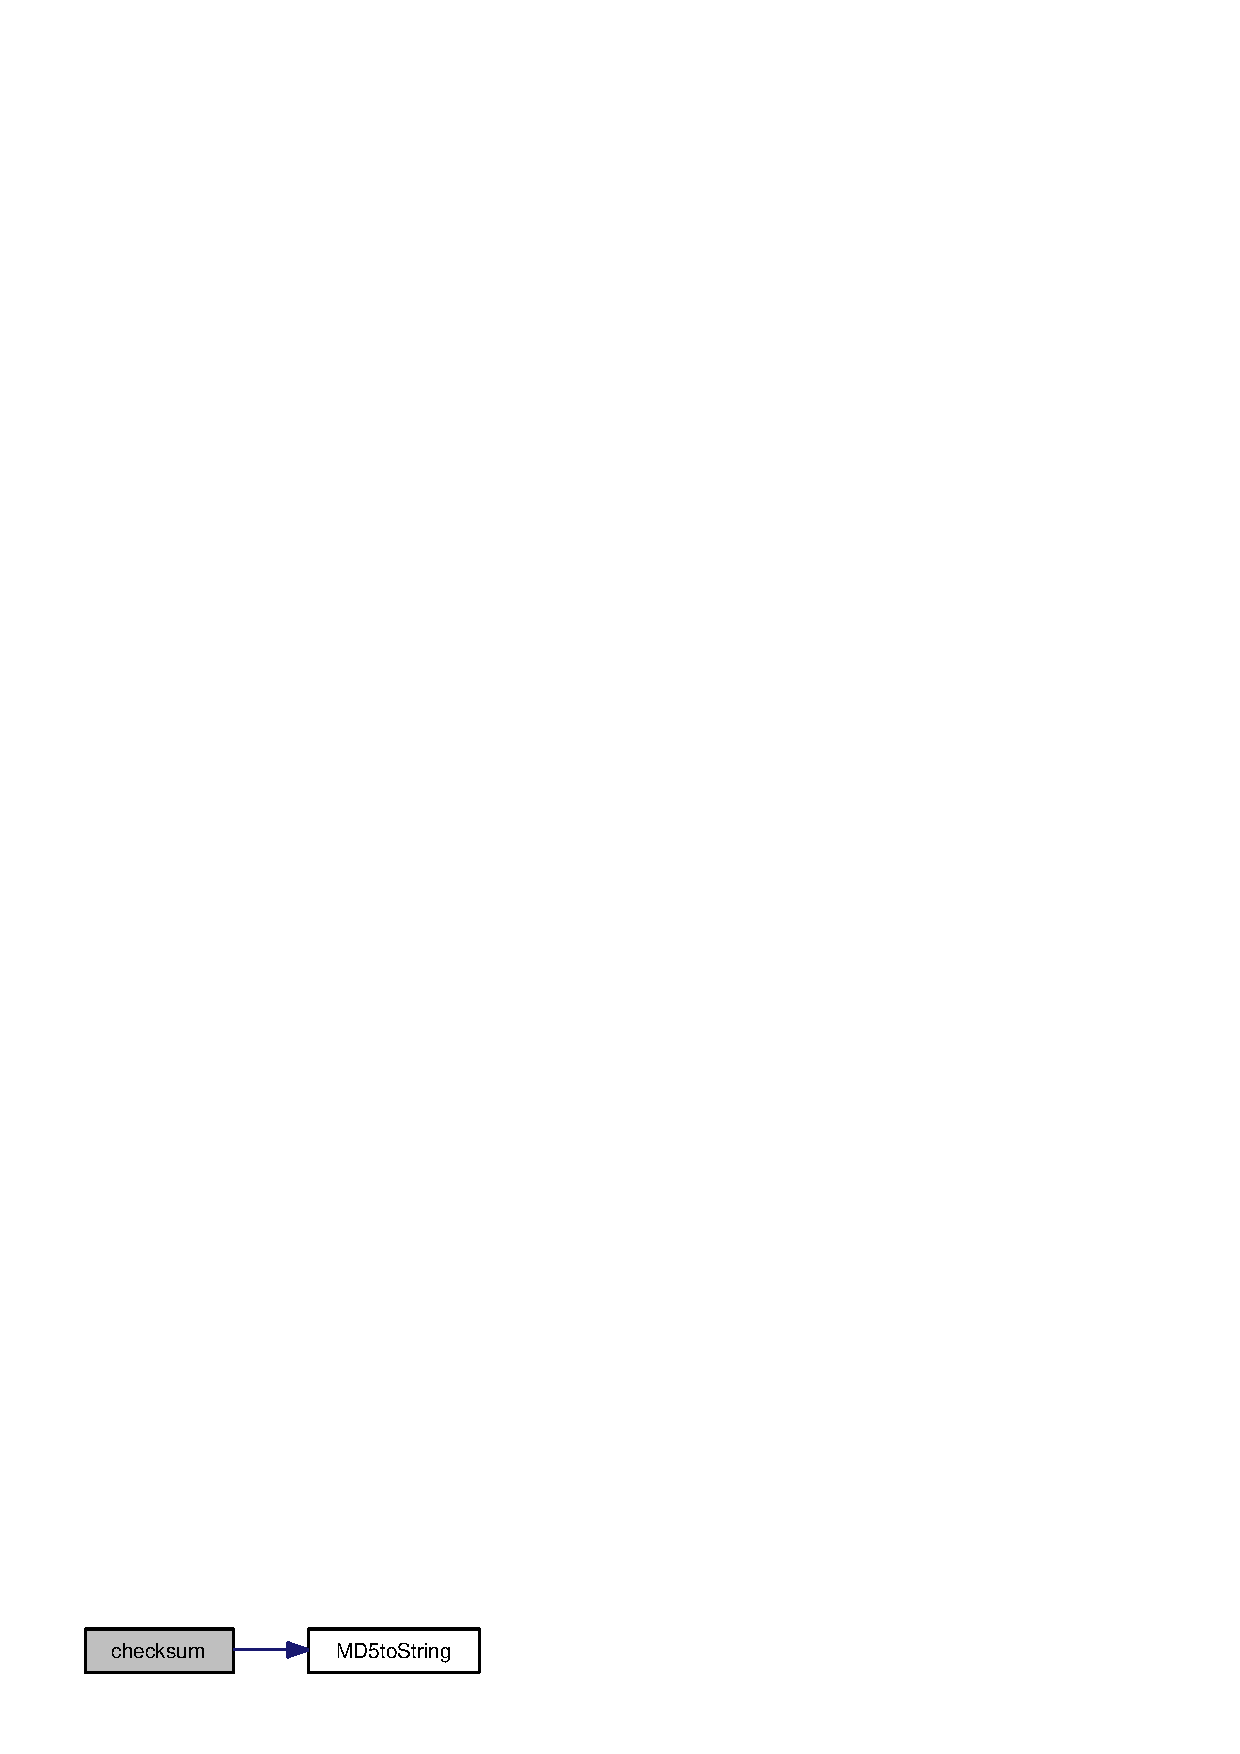
\includegraphics[width=234pt]{classorg_1_1smallfoot_1_1filexfer_1_1FileTransferWinch_affa1c48a18997a5ea5458d162d659c63_cgraph}
\end{center}
\end{figure}


\index{org\+::smallfoot\+::filexfer\+::\+File\+Transfer\+Winch@{org\+::smallfoot\+::filexfer\+::\+File\+Transfer\+Winch}!checksum@{checksum}}
\index{checksum@{checksum}!org\+::smallfoot\+::filexfer\+::\+File\+Transfer\+Winch@{org\+::smallfoot\+::filexfer\+::\+File\+Transfer\+Winch}}
\subsubsection[{checksum}]{\setlength{\rightskip}{0pt plus 5cm}static String checksum (
\begin{DoxyParamCaption}
\item[{String}]{file}
\end{DoxyParamCaption}
) throws java.\+security.\+No\+Such\+Algorithm\+Exception, java.\+io.\+File\+Not\+Found\+Exception, java.\+io.\+I\+O\+Exception\hspace{0.3cm}{\ttfamily [inline]}, {\ttfamily [static]}}\label{classorg_1_1smallfoot_1_1filexfer_1_1FileTransferWinch_a0009fd5377f2d667c4b58bc213ccde74}


Calculate an M\+D5 checksum. 

So in this function, given a filename, it passes execution to the \doxyref{checksum(\+File)}{p.}{classorg_1_1smallfoot_1_1filexfer_1_1FileTransferWinch_affa1c48a18997a5ea5458d162d659c63} function do do the actual work.


\begin{DoxyParams}{Parameters}
{\em file} & filename of the file to calculate \\
\hline
\end{DoxyParams}
\begin{DoxyReturn}{Returns}
checksum, as a string 
\end{DoxyReturn}


Definition at line 304 of file File\+Transfer\+Winch.\+java.



References File\+Transfer\+Winch.\+checksum().



Here is the call graph for this function\+:\nopagebreak
\begin{figure}[H]
\begin{center}
\leavevmode
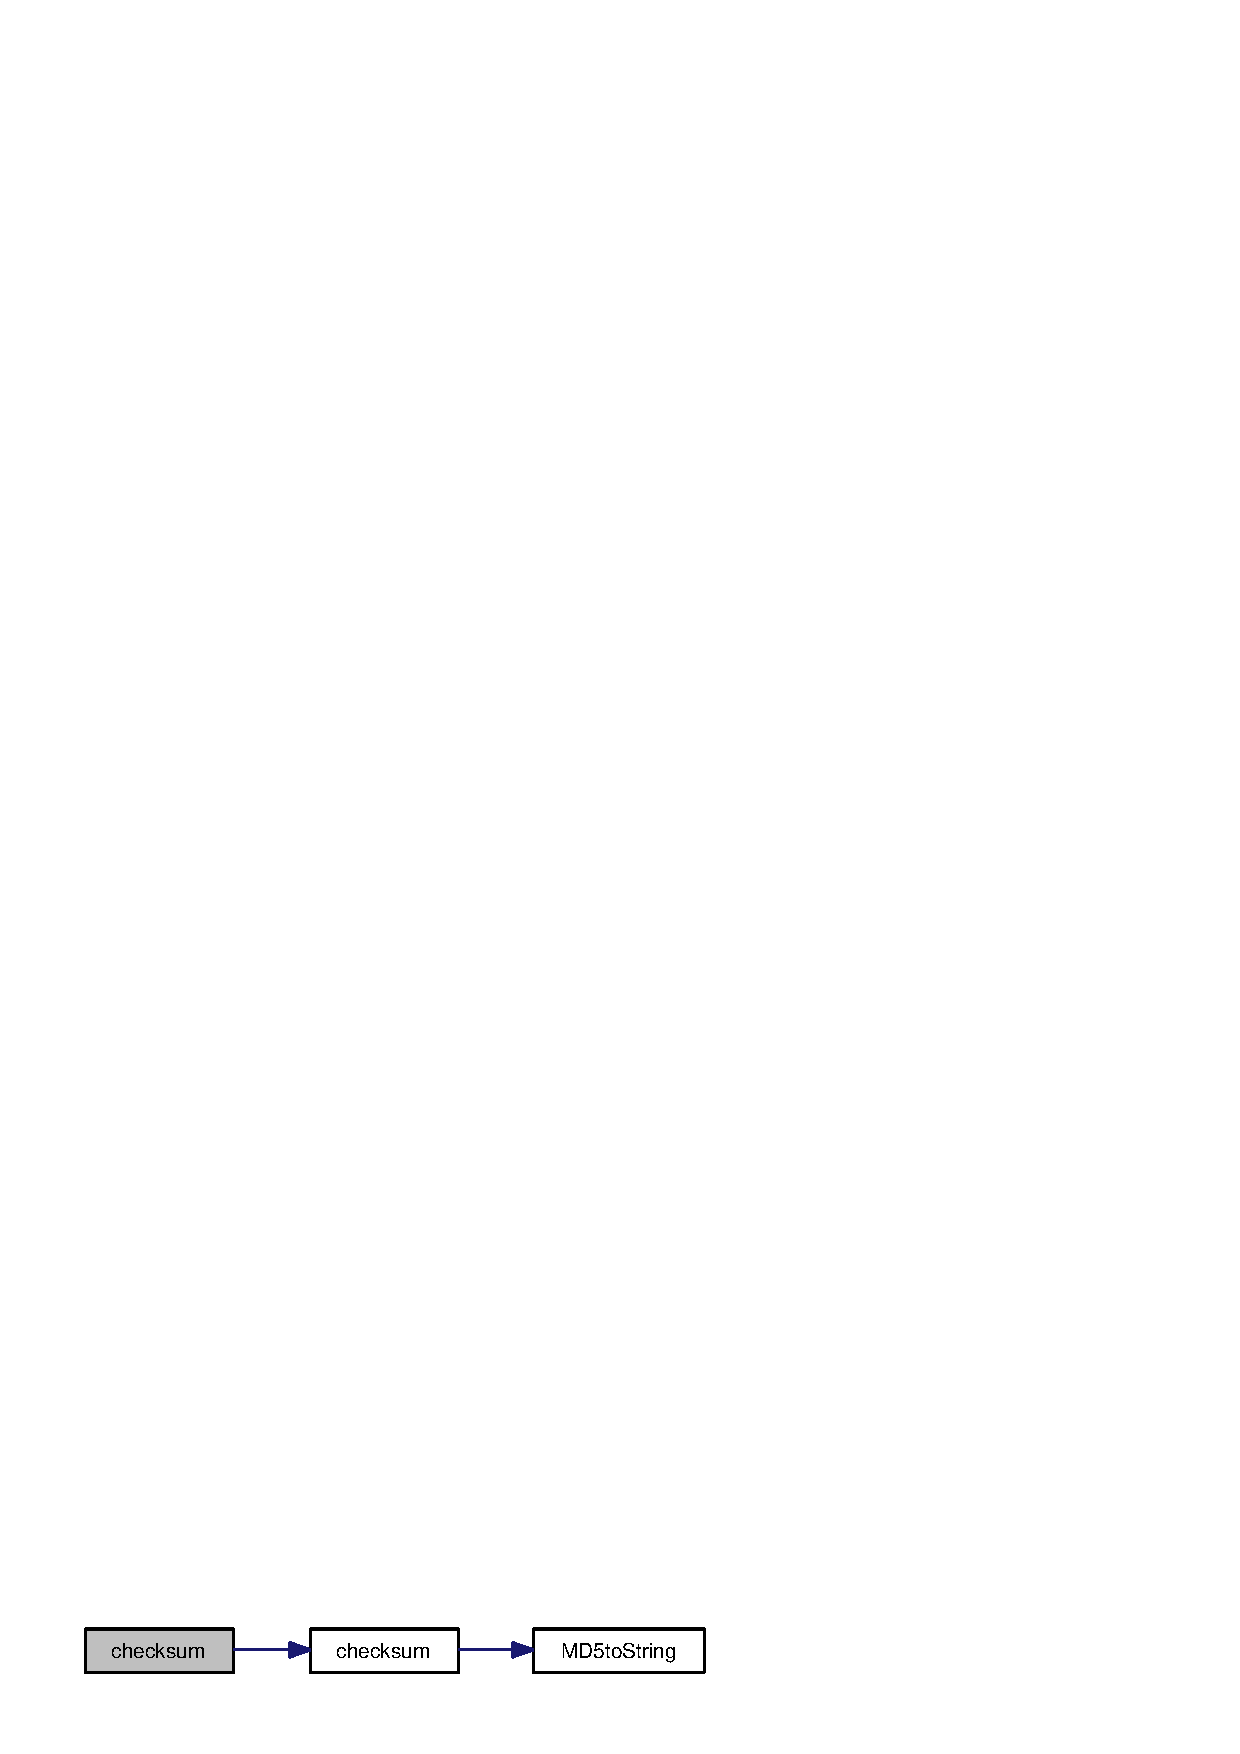
\includegraphics[width=342pt]{classorg_1_1smallfoot_1_1filexfer_1_1FileTransferWinch_a0009fd5377f2d667c4b58bc213ccde74_cgraph}
\end{center}
\end{figure}


\index{org\+::smallfoot\+::filexfer\+::\+File\+Transfer\+Winch@{org\+::smallfoot\+::filexfer\+::\+File\+Transfer\+Winch}!examples@{examples}}
\index{examples@{examples}!org\+::smallfoot\+::filexfer\+::\+File\+Transfer\+Winch@{org\+::smallfoot\+::filexfer\+::\+File\+Transfer\+Winch}}
\subsubsection[{examples}]{\setlength{\rightskip}{0pt plus 5cm}static String [$\,$] examples (
\begin{DoxyParamCaption}
\item[{java.\+net.\+U\+R\+L}]{url}
\end{DoxyParamCaption}
)\hspace{0.3cm}{\ttfamily [inline]}, {\ttfamily [static]}}\label{classorg_1_1smallfoot_1_1filexfer_1_1FileTransferWinch_ad6f50b0642401b9d8a38893ccc852bdf}


list one or more example U\+R\+Ls showing the available upload/download protocols 


\begin{DoxyParams}{Parameters}
{\em url} & a sample U\+R\+L showing user/pass/pathname \\
\hline
\end{DoxyParams}
\begin{DoxyReturn}{Returns}
array of examples using that U\+R\+L 
\end{DoxyReturn}


Definition at line 25 of file File\+Transfer\+Winch.\+java.

\index{org\+::smallfoot\+::filexfer\+::\+File\+Transfer\+Winch@{org\+::smallfoot\+::filexfer\+::\+File\+Transfer\+Winch}!M\+D5to\+String@{M\+D5to\+String}}
\index{M\+D5to\+String@{M\+D5to\+String}!org\+::smallfoot\+::filexfer\+::\+File\+Transfer\+Winch@{org\+::smallfoot\+::filexfer\+::\+File\+Transfer\+Winch}}
\subsubsection[{M\+D5to\+String}]{\setlength{\rightskip}{0pt plus 5cm}static String M\+D5to\+String (
\begin{DoxyParamCaption}
\item[{byte[$\,$]}]{digest}
\end{DoxyParamCaption}
)\hspace{0.3cm}{\ttfamily [inline]}, {\ttfamily [static]}}\label{classorg_1_1smallfoot_1_1filexfer_1_1FileTransferWinch_a947b12172158ca842bfe6bbae050da93}


convert a M\+D5 digest to a printable string. 

Part of \char`\"{}hey, why not include a checksum piece with everything?\char`\"{}

Public/\+Static because, hey, it might be useful elsewhere, and needs no state


\begin{DoxyParams}{Parameters}
{\em digest} & the resulting M\+D5 digest to convert to a string \\
\hline
\end{DoxyParams}
\begin{DoxyReturn}{Returns}
string representation of the digest 
\end{DoxyReturn}


Definition at line 243 of file File\+Transfer\+Winch.\+java.



Referenced by File\+Transfer\+Winch.\+checksum().

\index{org\+::smallfoot\+::filexfer\+::\+File\+Transfer\+Winch@{org\+::smallfoot\+::filexfer\+::\+File\+Transfer\+Winch}!upload@{upload}}
\index{upload@{upload}!org\+::smallfoot\+::filexfer\+::\+File\+Transfer\+Winch@{org\+::smallfoot\+::filexfer\+::\+File\+Transfer\+Winch}}
\subsubsection[{upload}]{\setlength{\rightskip}{0pt plus 5cm}abstract boolean upload (
\begin{DoxyParamCaption}
\item[{File}]{file, }
\item[{Vector$<$ String $>$}]{upload\+Notify}
\end{DoxyParamCaption}
) throws {\bf File\+Transfer\+Winch\+Exception}\hspace{0.3cm}{\ttfamily [abstract]}}\label{classorg_1_1smallfoot_1_1filexfer_1_1FileTransferWinch_a86dbba100f309afdccf3fc128da6a6cb}


upload a file using this \doxyref{File\+Transfer\+Winch}{p.}{classorg_1_1smallfoot_1_1filexfer_1_1FileTransferWinch}; errors in upload are handled via Exceptions 


\begin{DoxyParams}{Parameters}
{\em file} & the content to upload \\
\hline
{\em upload\+Notify} & array of identifiers (email address or jabber contacts) to list as notify recipients in the upload checksum file \\
\hline
\end{DoxyParams}
\begin{DoxyReturn}{Returns}
true if upload was checksum-\/certified; false is such facility isn't available (error if checksum is available and mismatches) 
\end{DoxyReturn}


Referenced by File\+Transfer\+Winch.\+upload().

\index{org\+::smallfoot\+::filexfer\+::\+File\+Transfer\+Winch@{org\+::smallfoot\+::filexfer\+::\+File\+Transfer\+Winch}!upload@{upload}}
\index{upload@{upload}!org\+::smallfoot\+::filexfer\+::\+File\+Transfer\+Winch@{org\+::smallfoot\+::filexfer\+::\+File\+Transfer\+Winch}}
\subsubsection[{upload}]{\setlength{\rightskip}{0pt plus 5cm}boolean upload (
\begin{DoxyParamCaption}
\item[{String}]{file, }
\item[{Vector$<$ String $>$}]{upload\+Notify}
\end{DoxyParamCaption}
) throws {\bf File\+Transfer\+Winch\+Exception}\hspace{0.3cm}{\ttfamily [inline]}}\label{classorg_1_1smallfoot_1_1filexfer_1_1FileTransferWinch_adfd6d2d56dee0986ab383e3735a2d0e1}


upload a file using this \doxyref{File\+Transfer\+Winch}{p.}{classorg_1_1smallfoot_1_1filexfer_1_1FileTransferWinch}; errors in upload are handled via Exceptions 


\begin{DoxyParams}{Parameters}
{\em file} & the content to upload \\
\hline
{\em upload\+Notify} & array of identifiers (email address or jabber contacts) to list as notify recipients in the upload checksum file \\
\hline
\end{DoxyParams}
\begin{DoxyReturn}{Returns}
true if upload was checksum-\/certified; false is such facility isn't available (error if checksum is available and mismatches) 
\end{DoxyReturn}


Definition at line 44 of file File\+Transfer\+Winch.\+java.



References File\+Transfer\+Winch.\+upload().



Here is the call graph for this function\+:\nopagebreak
\begin{figure}[H]
\begin{center}
\leavevmode
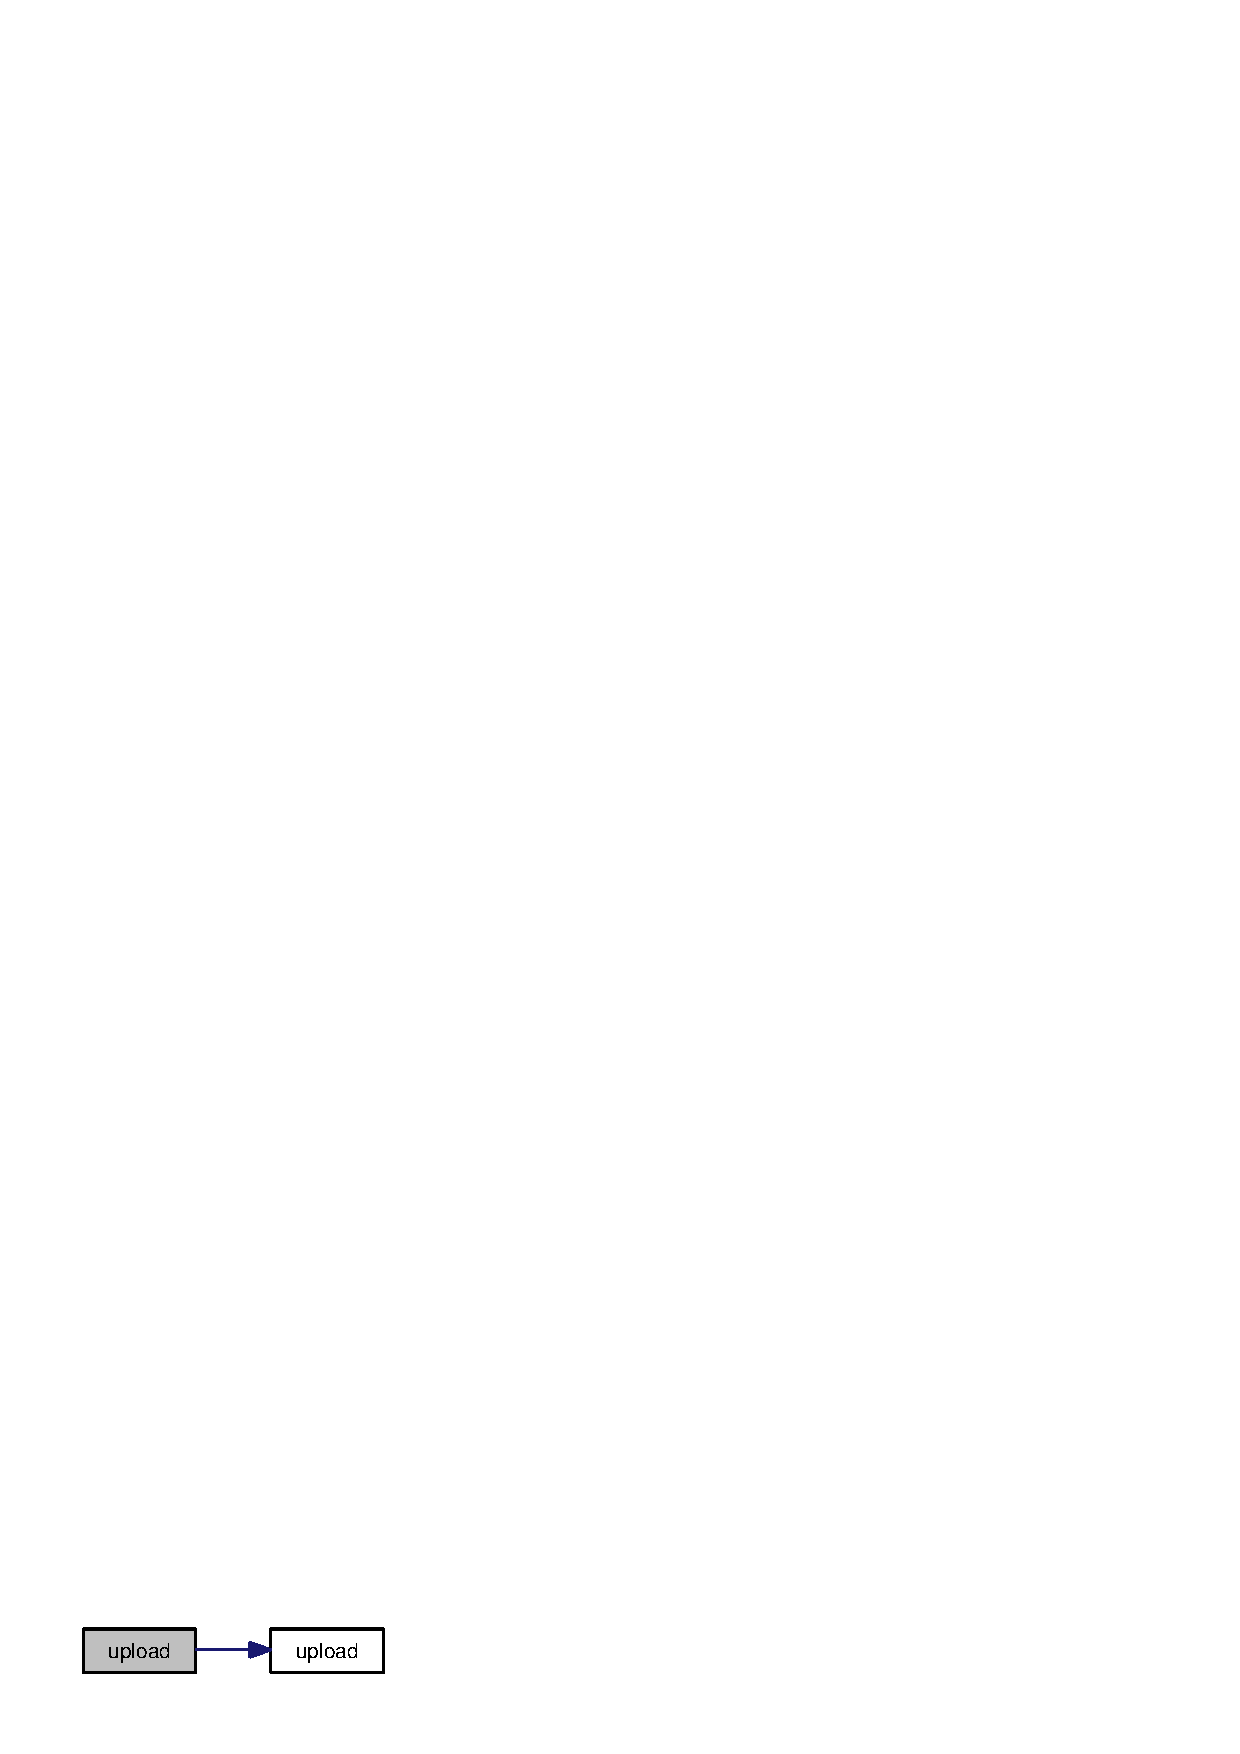
\includegraphics[width=188pt]{classorg_1_1smallfoot_1_1filexfer_1_1FileTransferWinch_adfd6d2d56dee0986ab383e3735a2d0e1_cgraph}
\end{center}
\end{figure}




The documentation for this class was generated from the following file\+:\begin{DoxyCompactItemize}
\item 
java/File\+Transfer\+Winch.\+java\end{DoxyCompactItemize}

\section{File\-Transfer\-Winch.\-File\-Transfer\-Winch\-Exception Class Reference}
\label{classorg_1_1smallfoot_1_1filexfer_1_1FileTransferWinch_1_1FileTransferWinchException}\index{File\-Transfer\-Winch.\-File\-Transfer\-Winch\-Exception@{File\-Transfer\-Winch.\-File\-Transfer\-Winch\-Exception}}


A base collector exception\-: \char`\"{}there was some exception in the File\-Transfer\-Winch class\char`\"{}; typically, more meaning and/or usefulness is reached by catching specific subclasses of this exception.  




Inheritance diagram for File\-Transfer\-Winch.\-File\-Transfer\-Winch\-Exception\-:\nopagebreak
\begin{figure}[H]
\begin{center}
\leavevmode
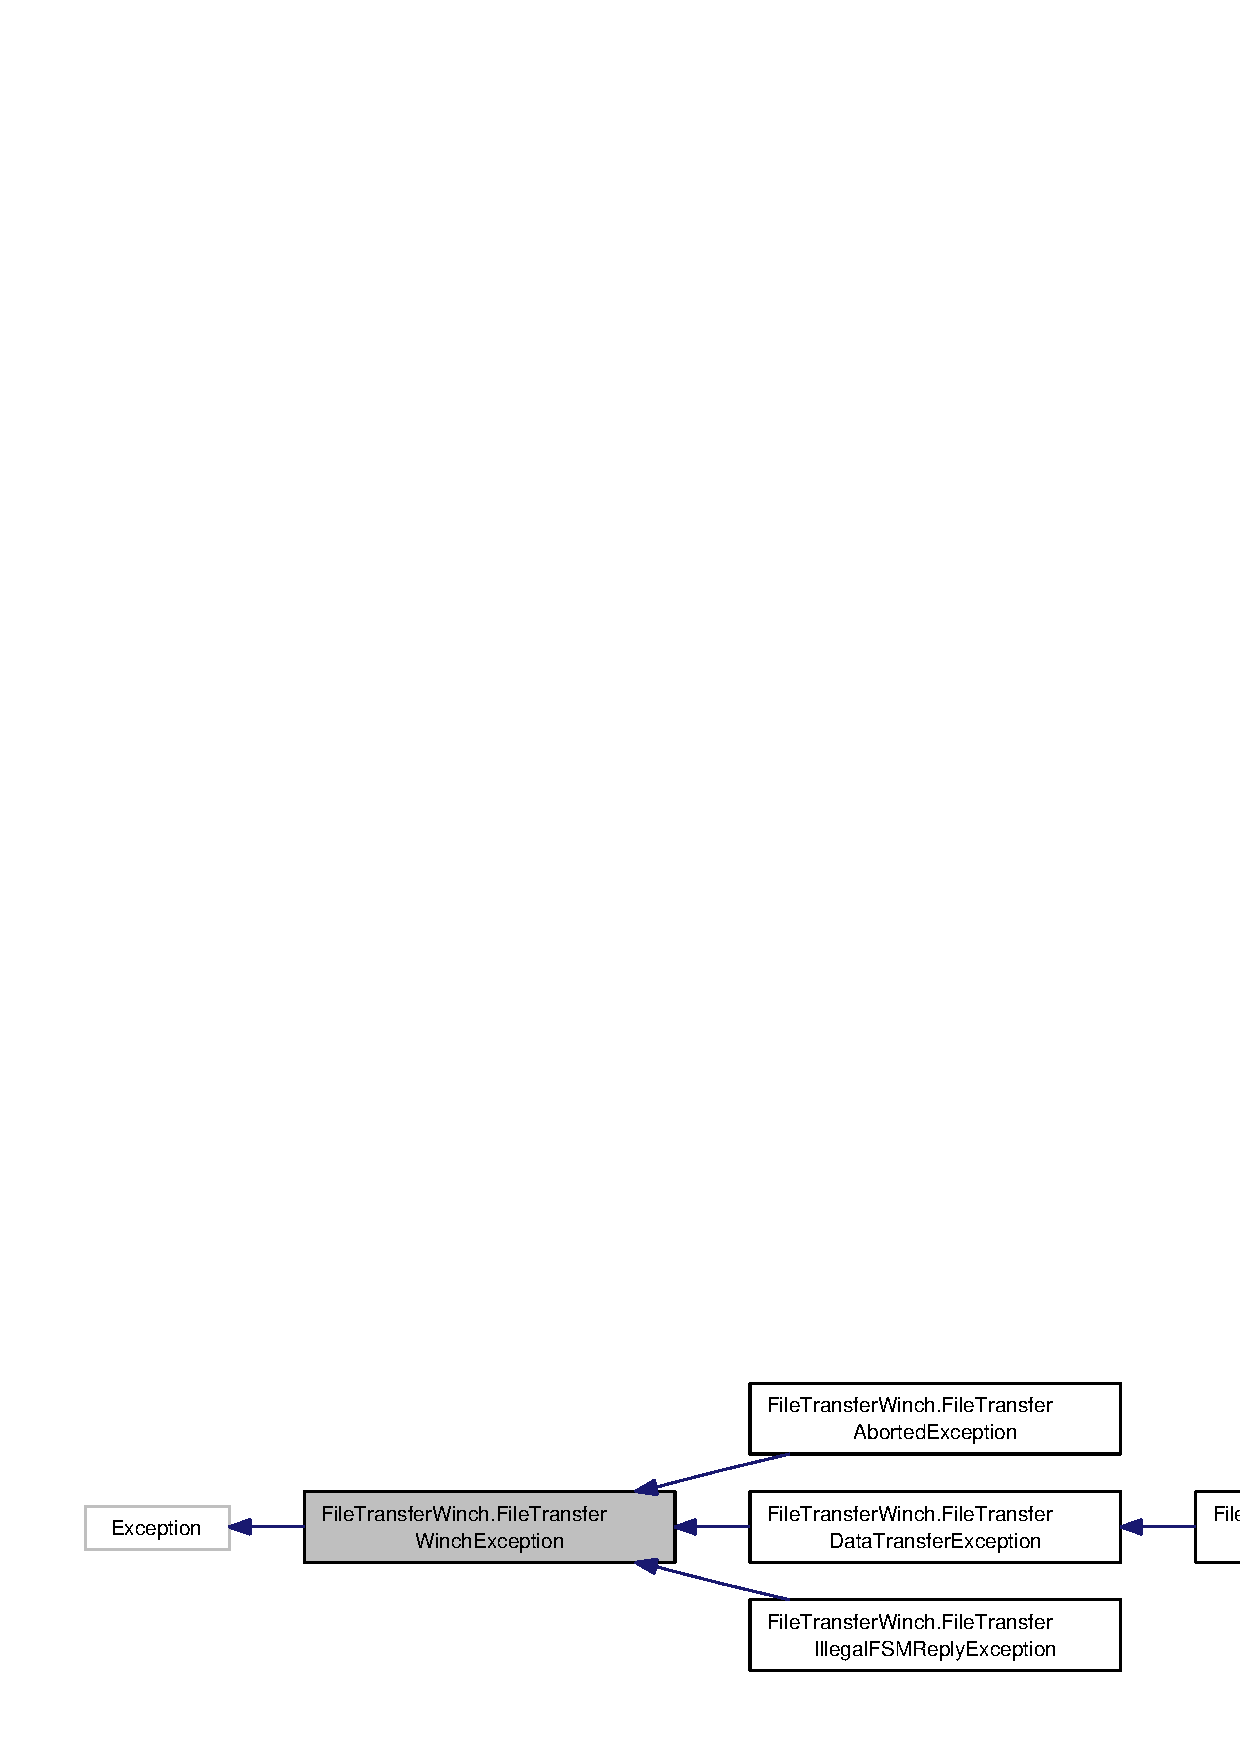
\includegraphics[width=350pt]{classorg_1_1smallfoot_1_1filexfer_1_1FileTransferWinch_1_1FileTransferWinchException__inherit__graph}
\end{center}
\end{figure}


Collaboration diagram for File\-Transfer\-Winch.\-File\-Transfer\-Winch\-Exception\-:\nopagebreak
\begin{figure}[H]
\begin{center}
\leavevmode
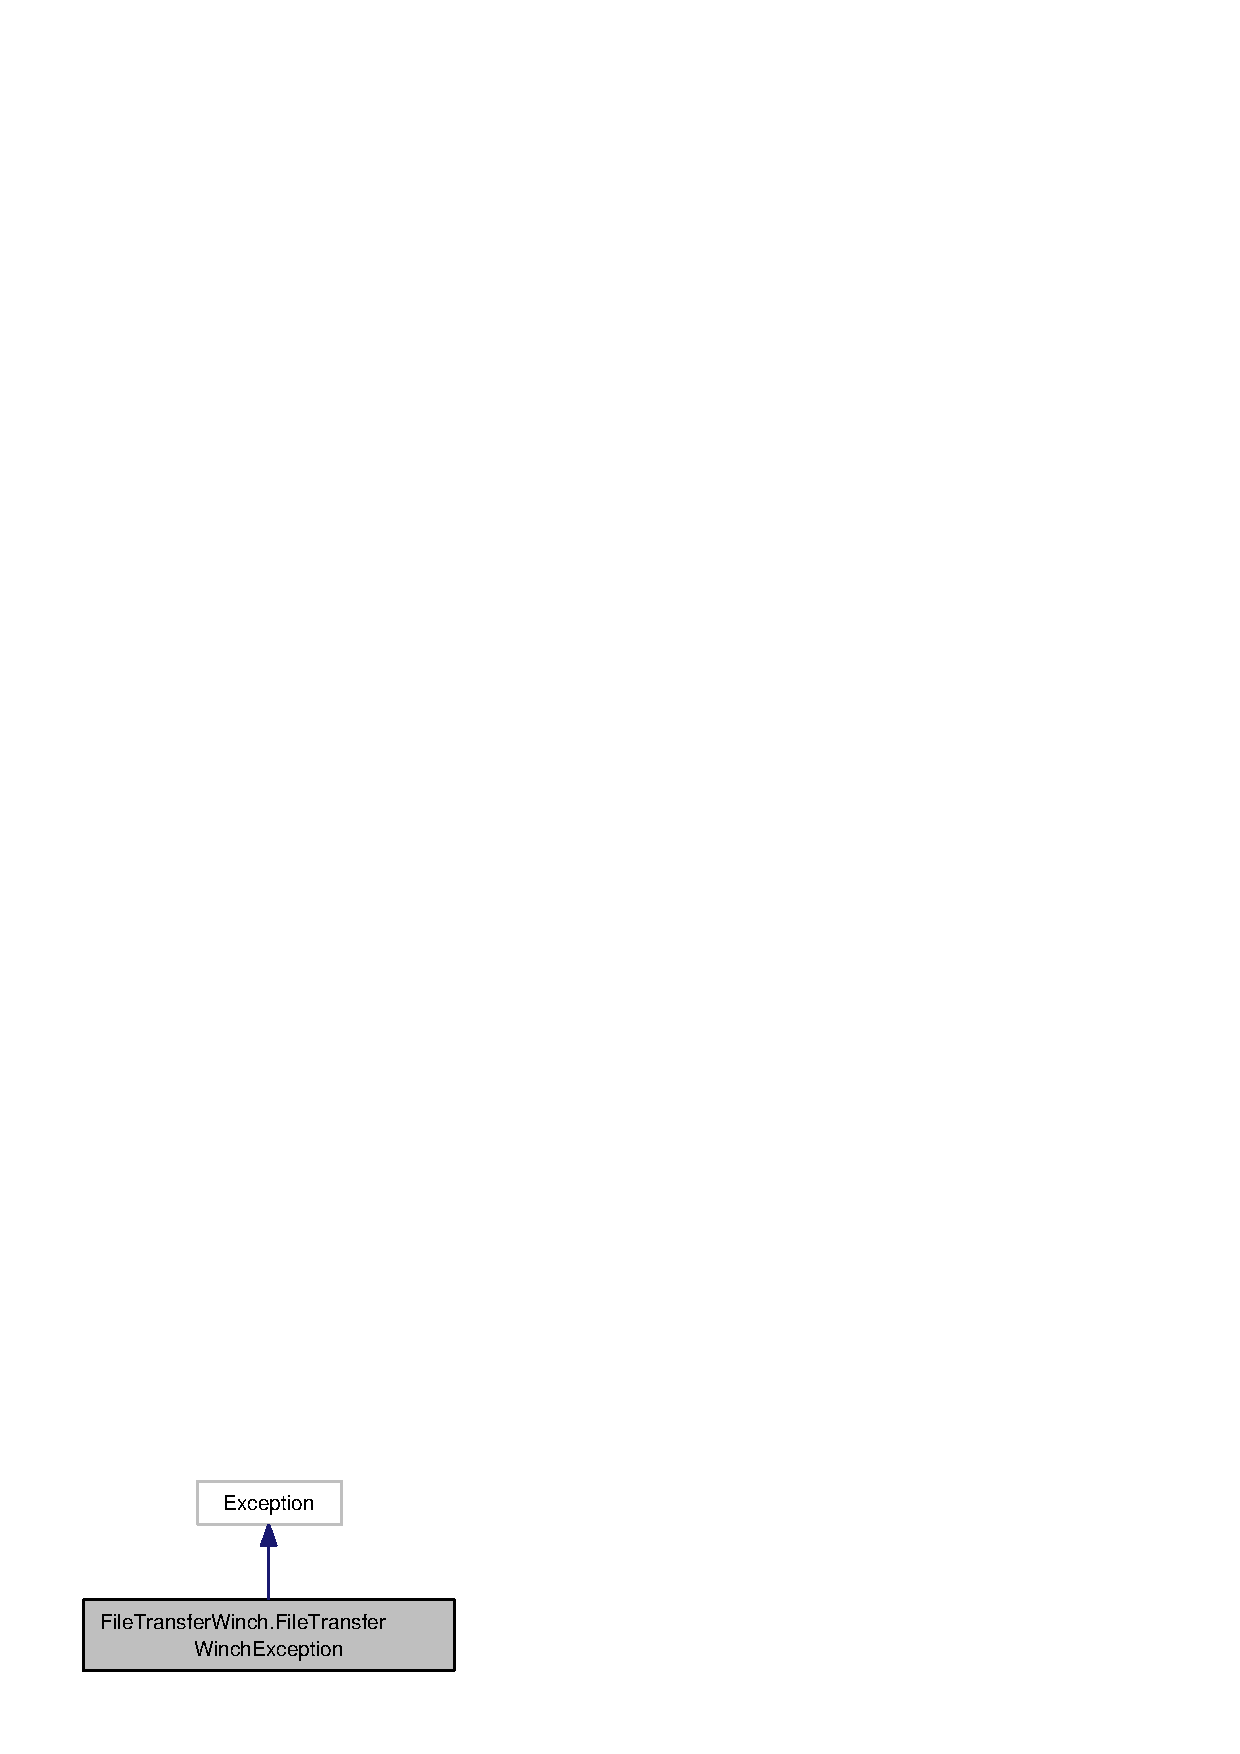
\includegraphics[width=222pt]{classorg_1_1smallfoot_1_1filexfer_1_1FileTransferWinch_1_1FileTransferWinchException__coll__graph}
\end{center}
\end{figure}
\subsection*{Public Member Functions}
\begin{DoxyCompactItemize}
\item 
{\bfseries File\-Transfer\-Winch\-Exception} (String s, Throwable t)\label{classorg_1_1smallfoot_1_1filexfer_1_1FileTransferWinch_1_1FileTransferWinchException_abf4a7354f578a7ff2783d7259d4a35c1}

\item 
{\bfseries File\-Transfer\-Winch\-Exception} (Throwable t)\label{classorg_1_1smallfoot_1_1filexfer_1_1FileTransferWinch_1_1FileTransferWinchException_a24d32d742afc2eb515a707f9086ae9a6}

\item 
{\bfseries File\-Transfer\-Winch\-Exception} (String s)\label{classorg_1_1smallfoot_1_1filexfer_1_1FileTransferWinch_1_1FileTransferWinchException_a28313c0c520cd234b6ccc2fafa72f8e5}

\end{DoxyCompactItemize}


\subsection{Detailed Description}
A base collector exception\-: \char`\"{}there was some exception in the File\-Transfer\-Winch class\char`\"{}; typically, more meaning and/or usefulness is reached by catching specific subclasses of this exception. 

Definition at line 50 of file File\-Transfer\-Winch.\-java.



The documentation for this class was generated from the following file\-:\begin{DoxyCompactItemize}
\item 
java/File\-Transfer\-Winch.\-java\end{DoxyCompactItemize}

\section{F\-T\-P4\-J Class Reference}
\label{classorg_1_1smallfoot_1_1filexfer_1_1FTP4J}\index{F\-T\-P4\-J@{F\-T\-P4\-J}}


Inheritance diagram for F\-T\-P4\-J\-:\nopagebreak
\begin{figure}[H]
\begin{center}
\leavevmode
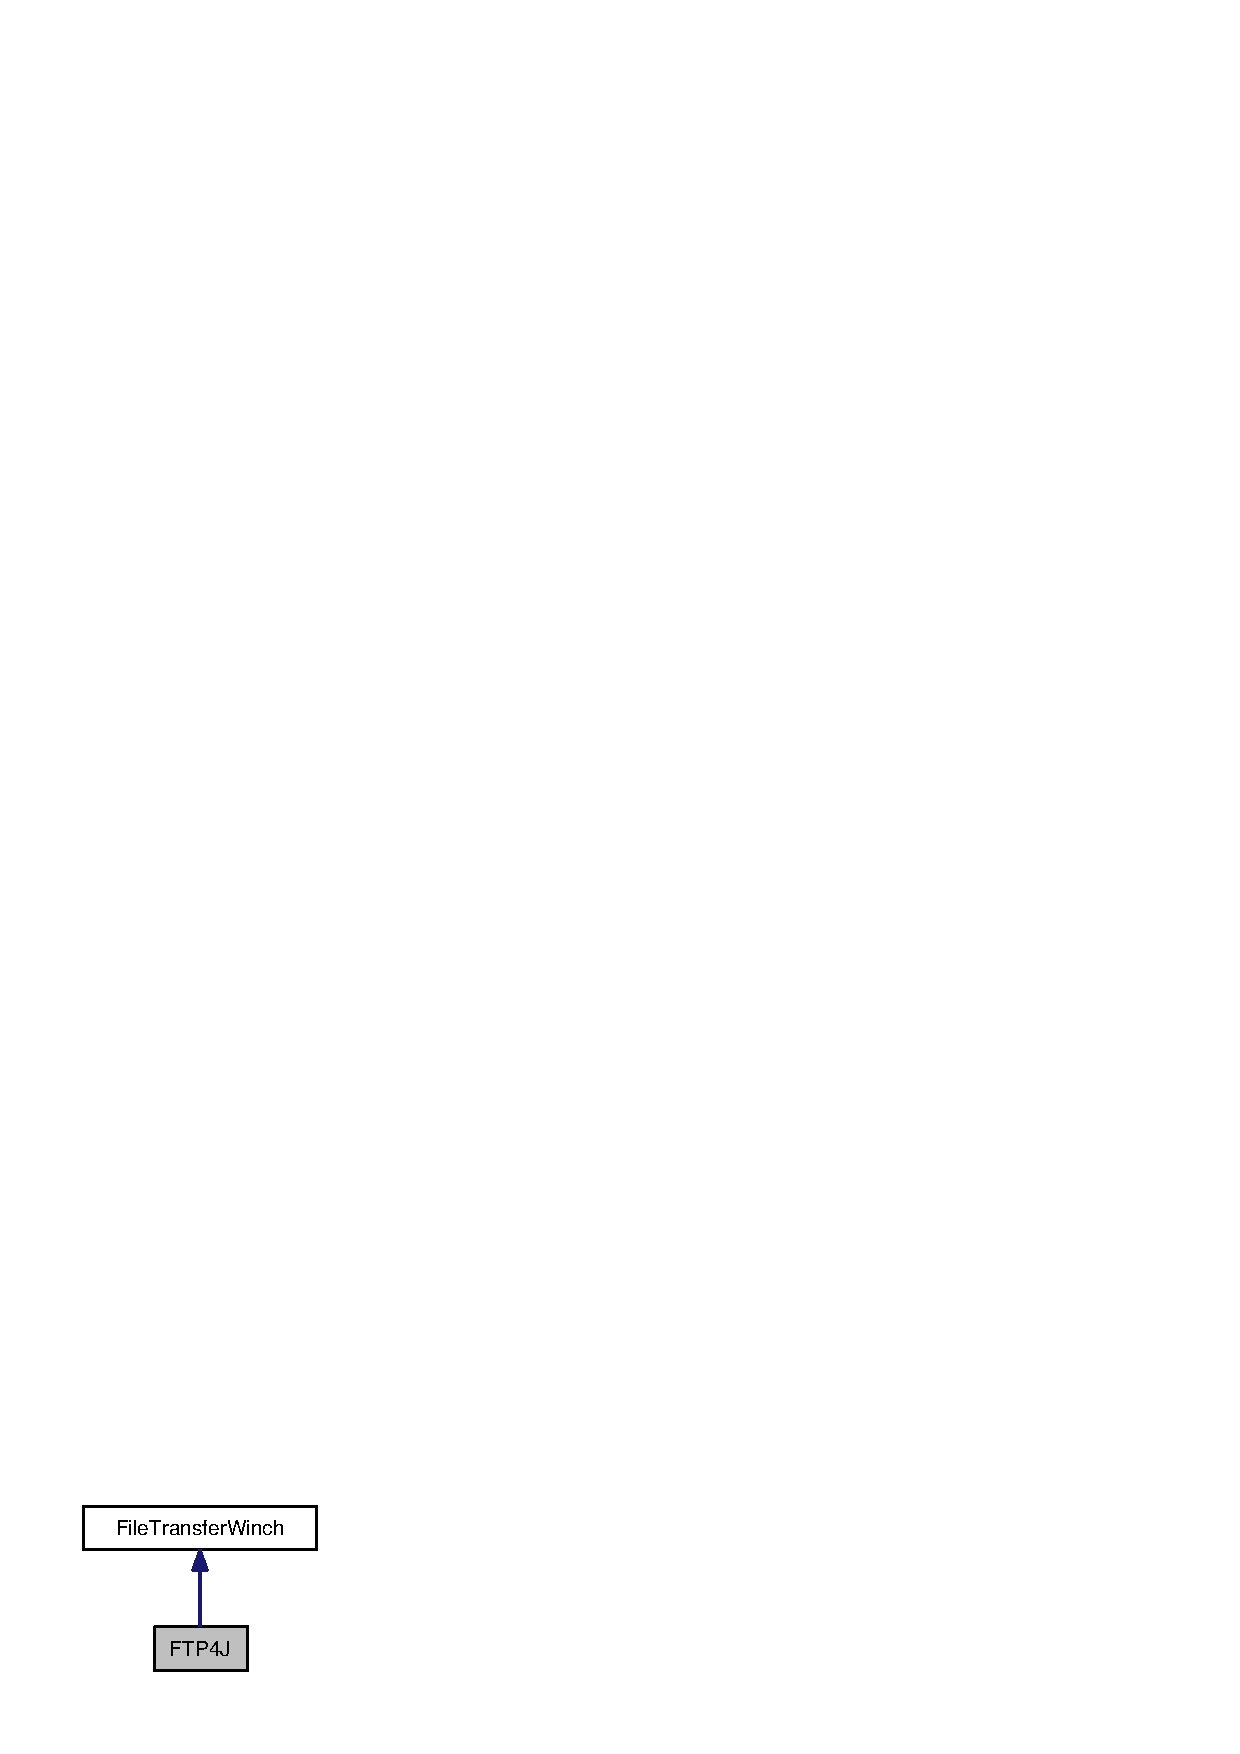
\includegraphics[width=156pt]{classorg_1_1smallfoot_1_1filexfer_1_1FTP4J__inherit__graph}
\end{center}
\end{figure}


Collaboration diagram for F\-T\-P4\-J\-:\nopagebreak
\begin{figure}[H]
\begin{center}
\leavevmode
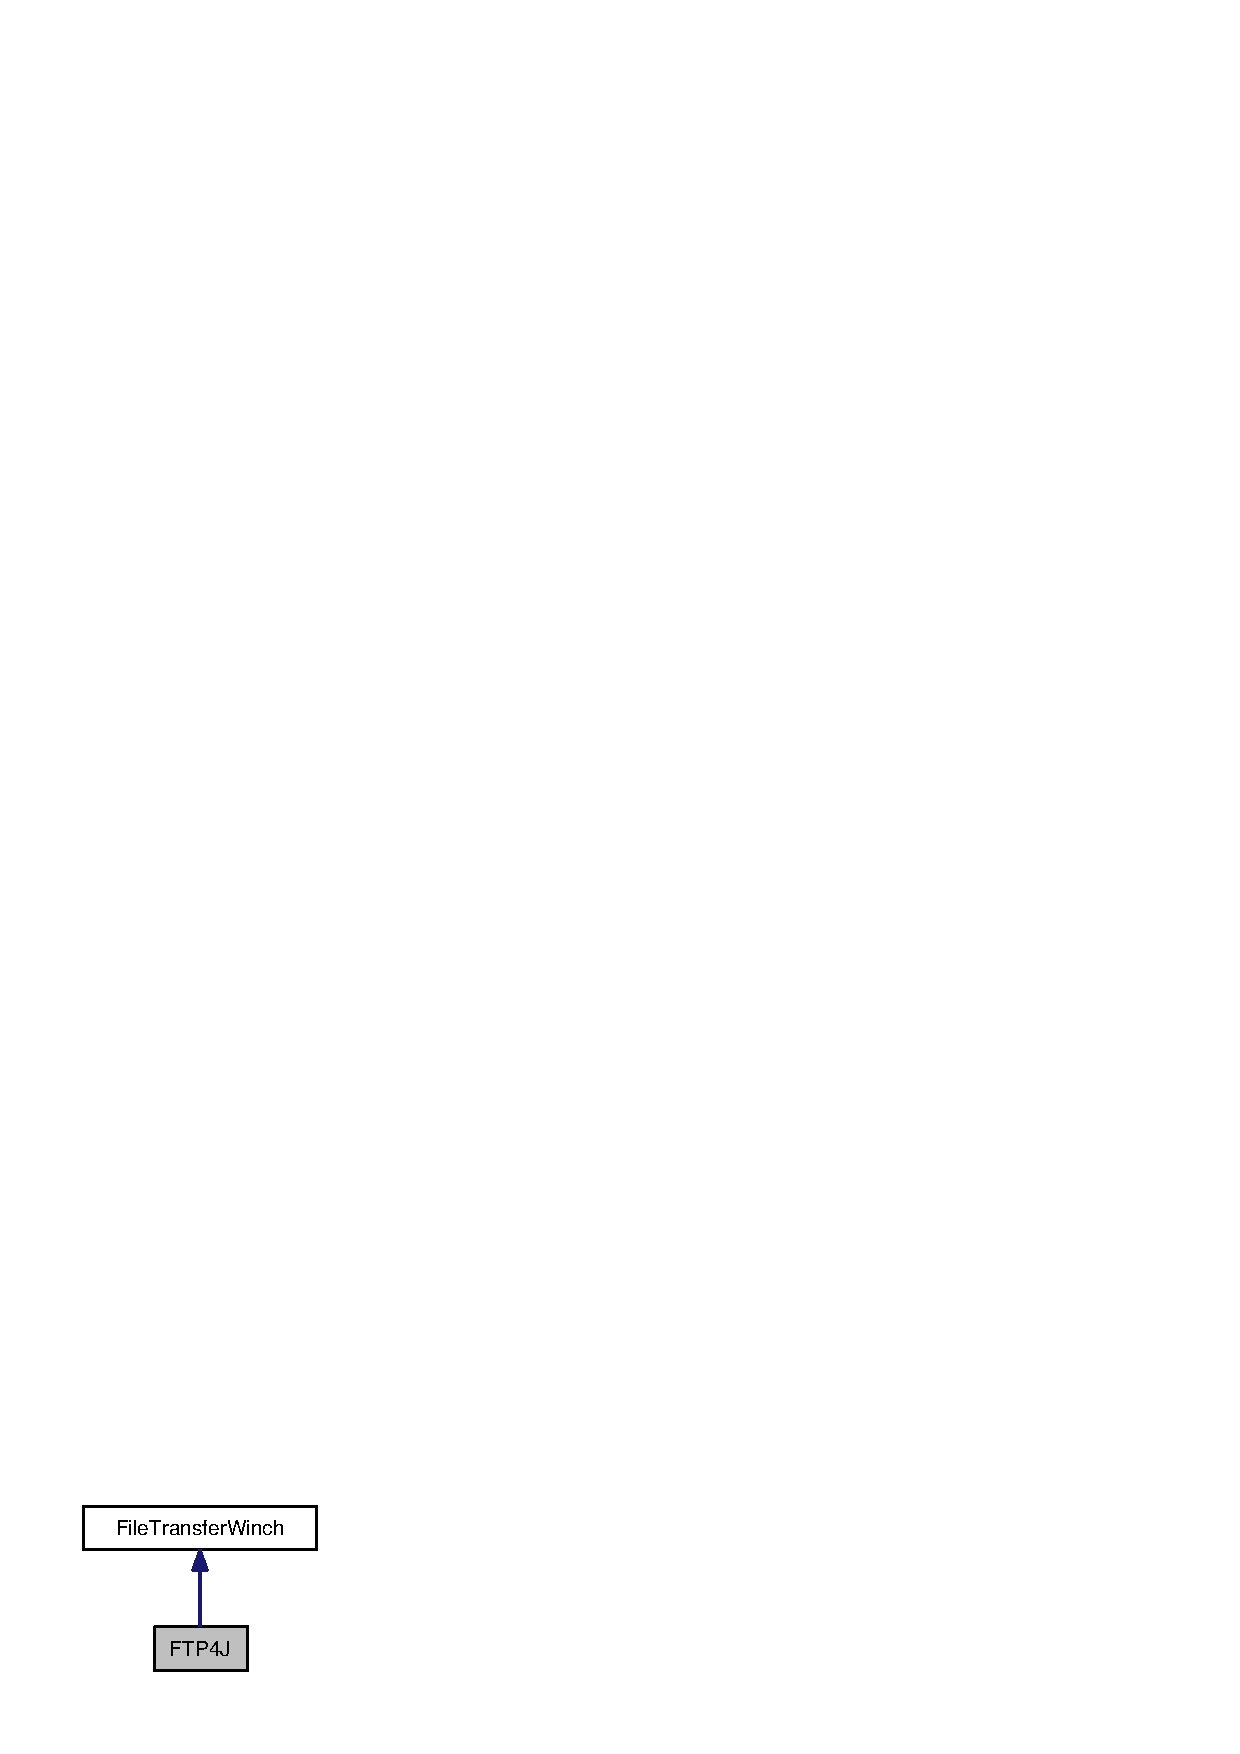
\includegraphics[width=156pt]{classorg_1_1smallfoot_1_1filexfer_1_1FTP4J__coll__graph}
\end{center}
\end{figure}
\subsection*{Public Member Functions}
\begin{DoxyCompactItemize}
\item 
{\bfseries F\-T\-P4\-J} (java.\-net.\-U\-R\-L u)\label{classorg_1_1smallfoot_1_1filexfer_1_1FTP4J_ad5bd367701ec46e8d0ba3f0ae3d83cae}

\item 
String {\bfseries get\-Pass} ()\label{classorg_1_1smallfoot_1_1filexfer_1_1FTP4J_a6cba30c67b9a7c8d4750e7e3108961c6}

\item 
String {\bfseries get\-User} ()\label{classorg_1_1smallfoot_1_1filexfer_1_1FTP4J_af8214ba89d8ad71194a2d69bea5cb808}

\item 
String {\bfseries name} ()\label{classorg_1_1smallfoot_1_1filexfer_1_1FTP4J_afa2149aced9d90555f788dfc81c23d15}

\item 
boolean {\bf upload} (File file, Vector$<$ String $>$ upload\-Notify)  throws File\-Transfer\-Winch\-Exception     
\begin{DoxyCompactList}\small\item\em Attempt an upload to the remote server. \end{DoxyCompactList}\end{DoxyCompactItemize}
\subsection*{Static Public Member Functions}
\begin{DoxyCompactItemize}
\item 
static String[$\,$] {\bf examples} (java.\-net.\-U\-R\-L url)
\begin{DoxyCompactList}\small\item\em list one or more example U\-R\-Ls showing the available upload/download protocols \end{DoxyCompactList}\item 
static boolean {\bfseries handles} (java.\-net.\-U\-R\-L u)\label{classorg_1_1smallfoot_1_1filexfer_1_1FTP4J_a4ef8d35ab128080eb511f7e26cd7ab7b}

\end{DoxyCompactItemize}
\subsection*{Additional Inherited Members}


\subsection{Detailed Description}


Definition at line 7 of file F\-T\-P4\-J.\-java.



\subsection{Member Function Documentation}
\index{org\-::smallfoot\-::filexfer\-::\-F\-T\-P4\-J@{org\-::smallfoot\-::filexfer\-::\-F\-T\-P4\-J}!examples@{examples}}
\index{examples@{examples}!org::smallfoot::filexfer::FTP4J@{org\-::smallfoot\-::filexfer\-::\-F\-T\-P4\-J}}
\subsubsection[{examples}]{\setlength{\rightskip}{0pt plus 5cm}static String [$\,$] examples (
\begin{DoxyParamCaption}
\item[{java.\-net.\-U\-R\-L}]{url}
\end{DoxyParamCaption}
)\hspace{0.3cm}{\ttfamily [inline]}, {\ttfamily [static]}}\label{classorg_1_1smallfoot_1_1filexfer_1_1FTP4J_ad6f50b0642401b9d8a38893ccc852bdf}


list one or more example U\-R\-Ls showing the available upload/download protocols 


\begin{DoxyParams}{Parameters}
{\em url} & a sample U\-R\-L showing user/pass/pathname \\
\hline
\end{DoxyParams}
\begin{DoxyReturn}{Returns}
array of examples using that U\-R\-L 
\end{DoxyReturn}


Definition at line 33 of file F\-T\-P4\-J.\-java.

\index{org\-::smallfoot\-::filexfer\-::\-F\-T\-P4\-J@{org\-::smallfoot\-::filexfer\-::\-F\-T\-P4\-J}!upload@{upload}}
\index{upload@{upload}!org::smallfoot::filexfer::FTP4J@{org\-::smallfoot\-::filexfer\-::\-F\-T\-P4\-J}}
\subsubsection[{upload}]{\setlength{\rightskip}{0pt plus 5cm}boolean upload (
\begin{DoxyParamCaption}
\item[{File}]{file, }
\item[{Vector$<$ String $>$}]{upload\-Notify}
\end{DoxyParamCaption}
) throws {\bf File\-Transfer\-Winch\-Exception}\hspace{0.3cm}{\ttfamily [inline]}}\label{classorg_1_1smallfoot_1_1filexfer_1_1FTP4J_afa3dfccec4b989cafc56103eb1ee82a6}


Attempt an upload to the remote server. 

Initially very basic, this can be extended for all the intelligence we need to get data through.

This function, given a filename, connects to an F\-T\-P server and attempts to store the file. Initially the username and password are defaulted to those usable to upload from P\-A\-K\-\_\-\-R\-E\-D, but later (when i can look at U\-R\-L factories) this can be extended. The capability will be preserved to give the function a list of statuses and a position so that a later threaded design can try a number of uploads in parallel, ditching all but the most efficient\-: on connection, so status-\/indiciates; on successful 1-\/k upload with a temp filename, status-\/indicates finished 1k, and checks whether others are -- if others are ahead of it, status-\/indicates as \char`\"{}losing\char`\"{} and deletes its temp file; others behind it will so-\/suicide; if it's the non-\/losing, then this thread \char`\"{}continues\char`\"{} the upload from 1k, or deletes/restarts if continuation is impossible. In that way, the fastest connection continues, the others give up, timeouts are handled implicitly.

Where possible, checksum post-\/upload is verified

Where possible, a checksum file \{filename\}.sum is uploaded Where possible, a manifest X\-M\-L file is sent (my hostname, my user I\-D, any tasks or objectives, etc)


\begin{DoxyParams}{Parameters}
{\em file} & filename to upload \\
\hline
{\em upload\-Notify} & array of identifiers (email address or jabber contacts) to list as notify recipients in the upload checksum file \\
\hline
\end{DoxyParams}
\begin{DoxyReturn}{Returns}
\char`\"{}\-O\-K, \#\#\char`\"{}, \char`\"{}\-F\-A\-I\-L, \#\#\char`\"{}, \char`\"{}\-U\-N\-K\-N\-O\-W\-N\char`\"{} based on results (where \char`\"{}\#\#\char`\"{} is a line number of variable length) 
\end{DoxyReturn}


Definition at line 66 of file F\-T\-P4\-J.\-java.



References File\-Transfer\-Winch.\-checksum().



Here is the call graph for this function\-:\nopagebreak
\begin{figure}[H]
\begin{center}
\leavevmode
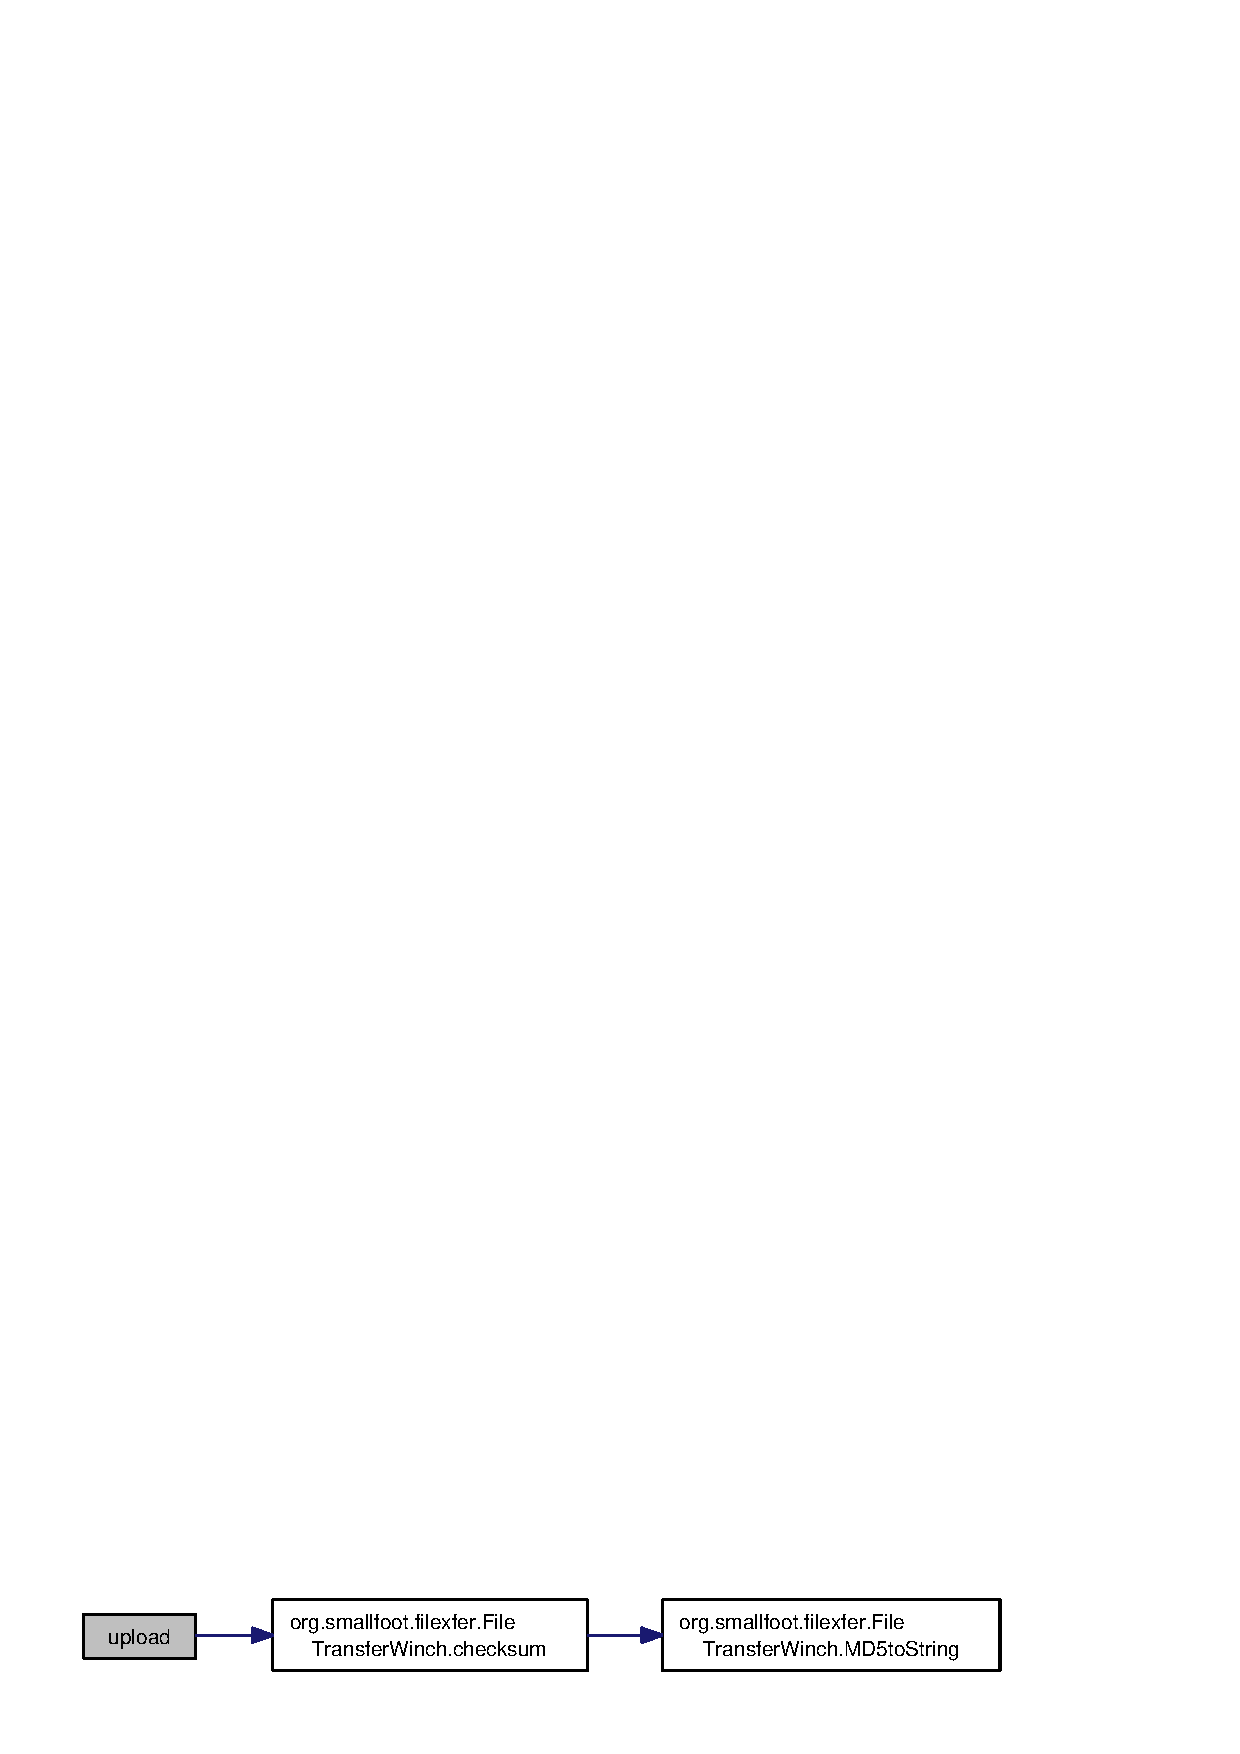
\includegraphics[width=350pt]{classorg_1_1smallfoot_1_1filexfer_1_1FTP4J_afa3dfccec4b989cafc56103eb1ee82a6_cgraph}
\end{center}
\end{figure}




The documentation for this class was generated from the following file\-:\begin{DoxyCompactItemize}
\item 
java/F\-T\-P4\-J.\-java\end{DoxyCompactItemize}

\section{Handler Class Reference}
\label{classorg_1_1smallfoot_1_1filexfer_1_1sftp_1_1Handler}\index{Handler@{Handler}}


Inheritance diagram for Handler\+:\nopagebreak
\begin{figure}[H]
\begin{center}
\leavevmode
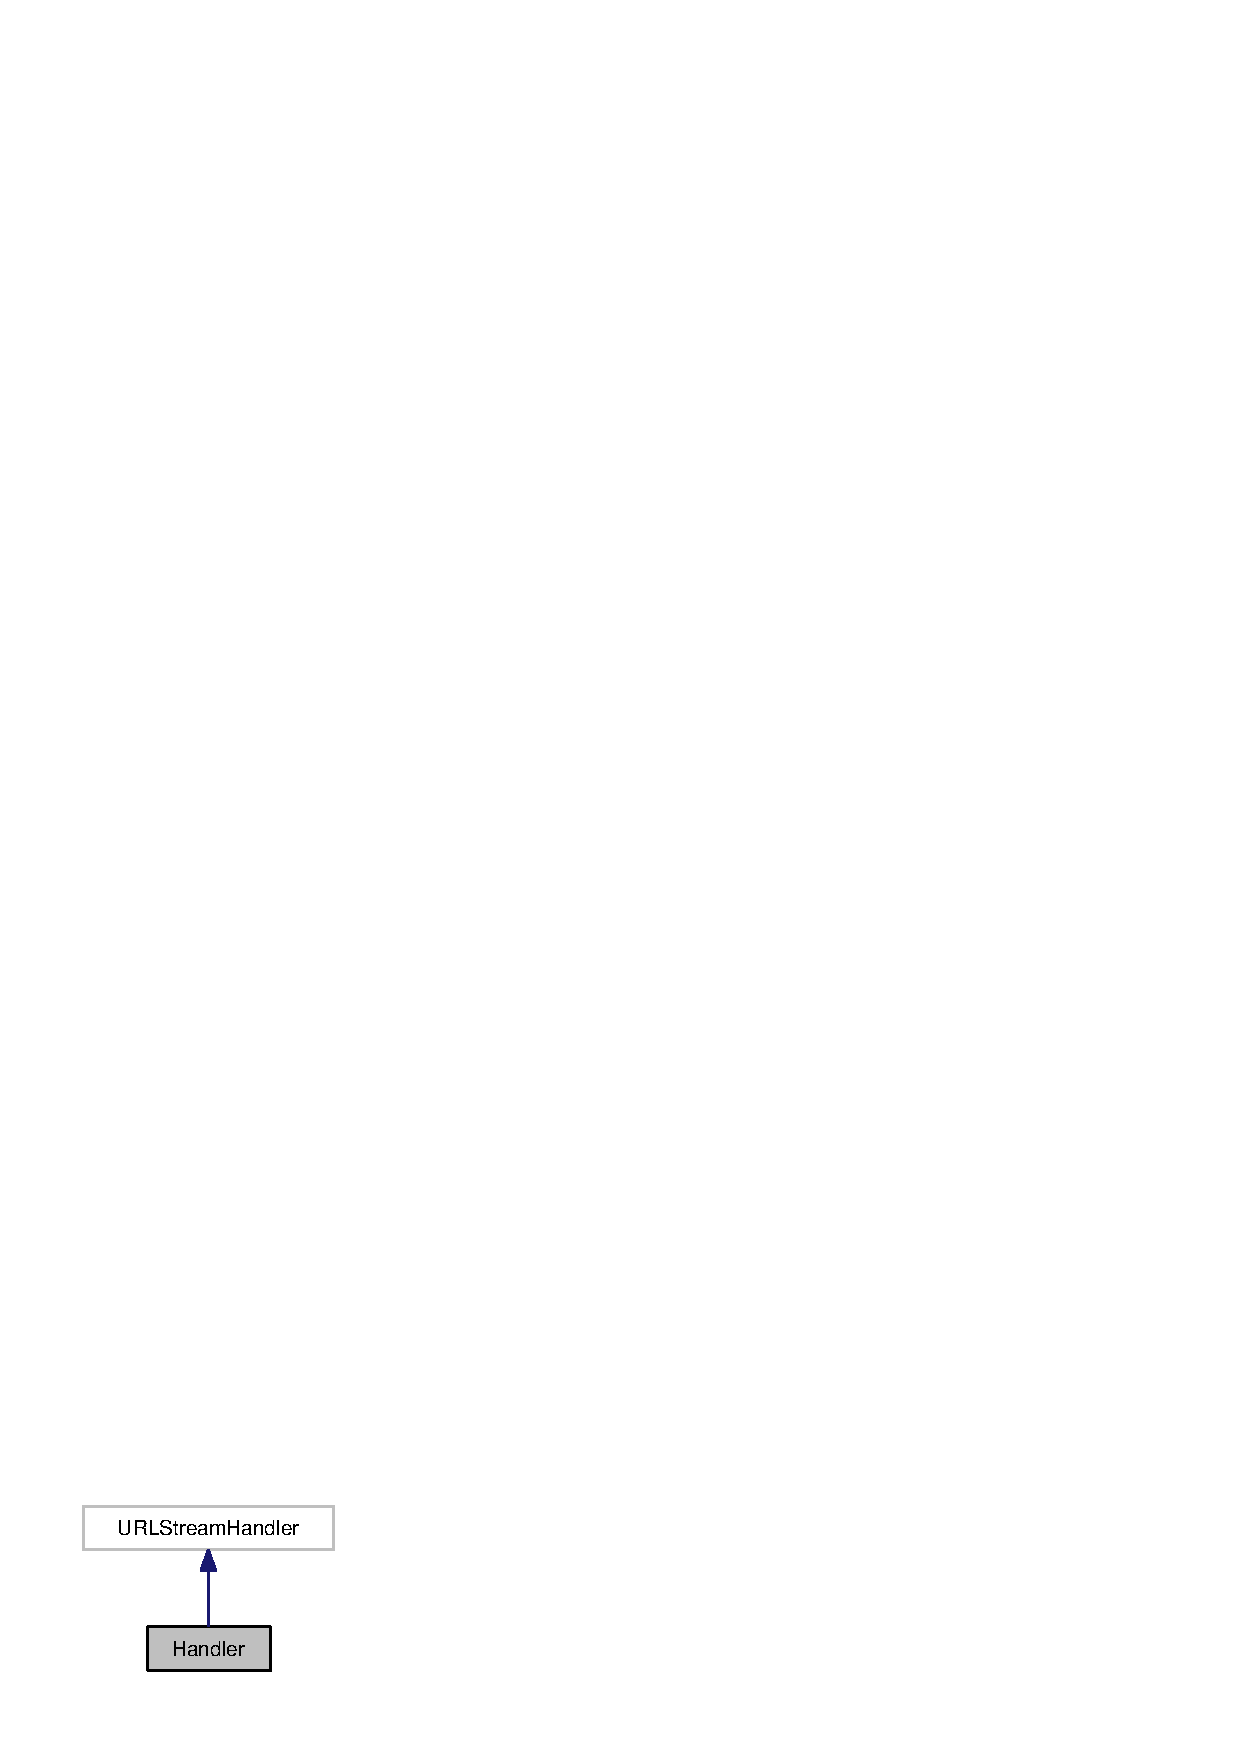
\includegraphics[width=164pt]{classorg_1_1smallfoot_1_1filexfer_1_1sftp_1_1Handler__inherit__graph}
\end{center}
\end{figure}


Collaboration diagram for Handler\+:\nopagebreak
\begin{figure}[H]
\begin{center}
\leavevmode
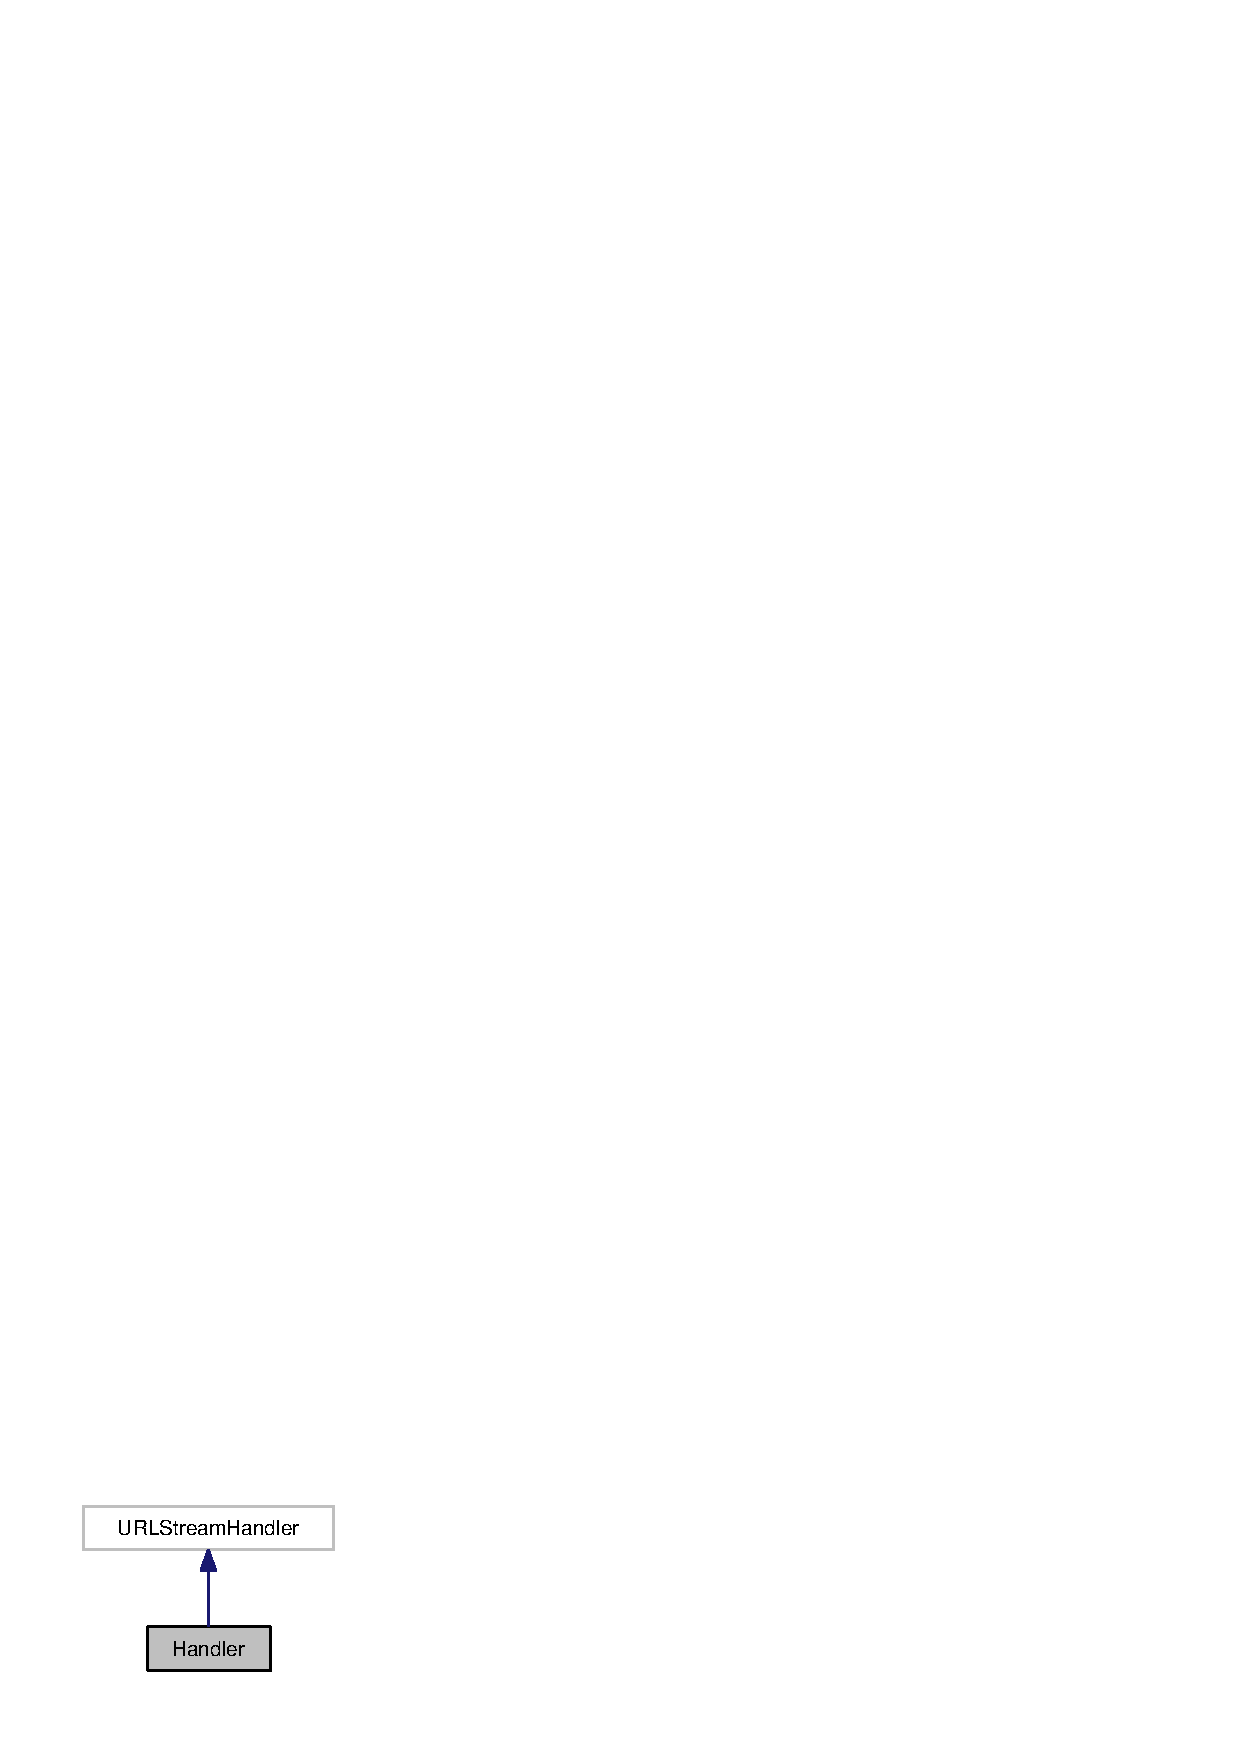
\includegraphics[width=164pt]{classorg_1_1smallfoot_1_1filexfer_1_1sftp_1_1Handler__coll__graph}
\end{center}
\end{figure}
\subsection*{Protected Member Functions}
\begin{DoxyCompactItemize}
\item 
java.\+net.\+U\+R\+L\+Connection {\bf open\+Connection} (java.\+net.\+U\+R\+L url)
\begin{DoxyCompactList}\small\item\em open\+Connection(java.\+net.\+U\+R\+L) overrides java.\+net.\+U\+R\+L\+Stream\+Handler.\+open\+Connection(\+U\+R\+L) by wrapping a apache-\/commons-\/net-\/sftp client \end{DoxyCompactList}\end{DoxyCompactItemize}


\subsection{Detailed Description}


Definition at line 8 of file Handler.\+java.



\subsection{Member Function Documentation}
\index{org\+::smallfoot\+::filexfer\+::sftp\+::\+Handler@{org\+::smallfoot\+::filexfer\+::sftp\+::\+Handler}!open\+Connection@{open\+Connection}}
\index{open\+Connection@{open\+Connection}!org\+::smallfoot\+::filexfer\+::sftp\+::\+Handler@{org\+::smallfoot\+::filexfer\+::sftp\+::\+Handler}}
\subsubsection[{open\+Connection}]{\setlength{\rightskip}{0pt plus 5cm}java.\+net.\+U\+R\+L\+Connection open\+Connection (
\begin{DoxyParamCaption}
\item[{java.\+net.\+U\+R\+L}]{url}
\end{DoxyParamCaption}
)\hspace{0.3cm}{\ttfamily [inline]}, {\ttfamily [protected]}}\label{classorg_1_1smallfoot_1_1filexfer_1_1sftp_1_1Handler_a1ef9160a9dbe5c066dd23e0f2cde39da}


open\+Connection(java.\+net.\+U\+R\+L) overrides java.\+net.\+U\+R\+L\+Stream\+Handler.\+open\+Connection(\+U\+R\+L) by wrapping a apache-\/commons-\/net-\/sftp client 

\begin{DoxyReturn}{Returns}
populated connection as \doxyref{org.\+smallfoot.\+filexfer.\+sftp.\+S\+F\+T\+P\+U\+R\+L\+Connection(\+Connection)}{p.}{classorg_1_1smallfoot_1_1filexfer_1_1sftp_1_1SFTPURLConnection} 
\end{DoxyReturn}

\begin{DoxyParams}{Parameters}
{\em url} & U\+R\+L to connect to \\
\hline
\end{DoxyParams}


Definition at line 16 of file Handler.\+java.



The documentation for this class was generated from the following file\+:\begin{DoxyCompactItemize}
\item 
java/sftp/{\bf Handler.\+java}\end{DoxyCompactItemize}

\section{S\-F\-T\-P\-U\-R\-L\-Connection Class Reference}
\label{classorg_1_1smallfoot_1_1filexfer_1_1sftp_1_1SFTPURLConnection}\index{S\-F\-T\-P\-U\-R\-L\-Connection@{S\-F\-T\-P\-U\-R\-L\-Connection}}


Inheritance diagram for S\-F\-T\-P\-U\-R\-L\-Connection\-:\nopagebreak
\begin{figure}[H]
\begin{center}
\leavevmode
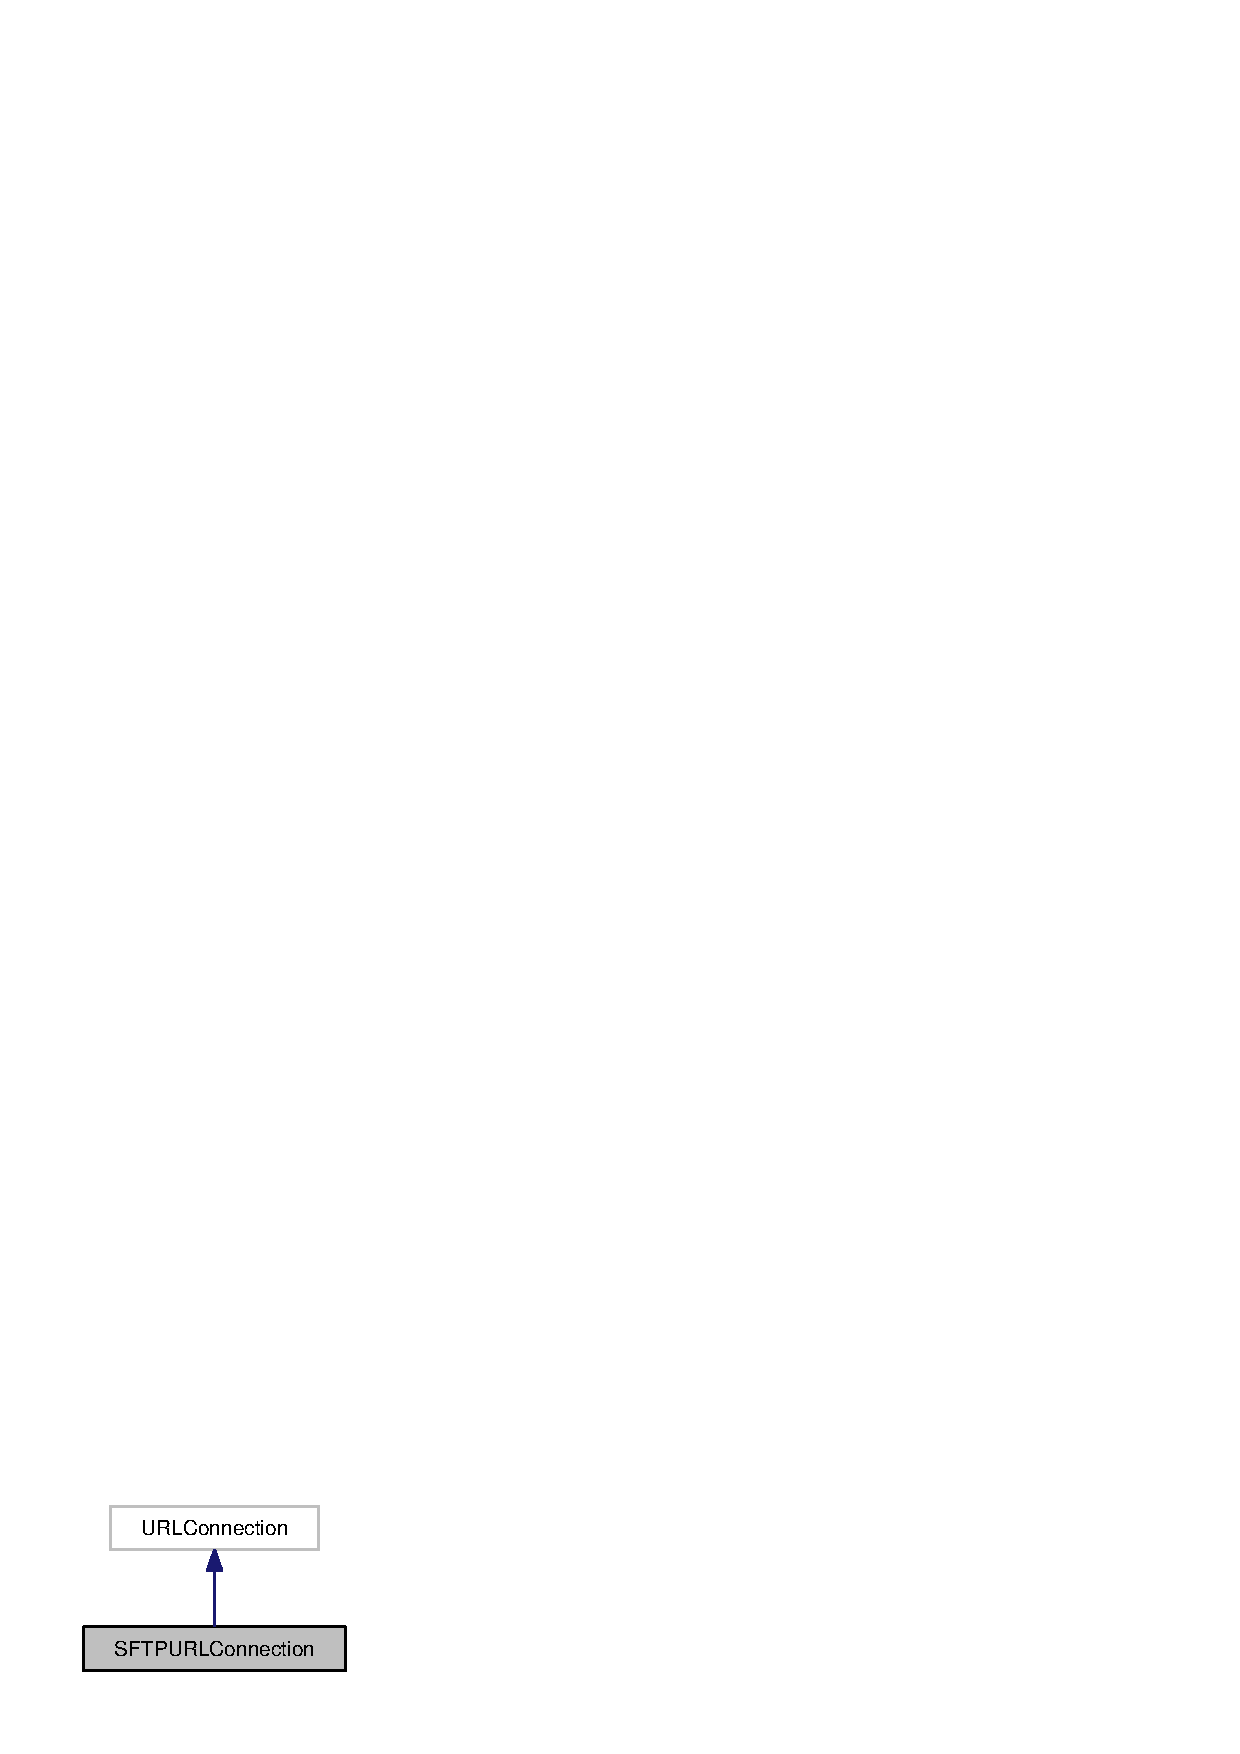
\includegraphics[width=170pt]{classorg_1_1smallfoot_1_1filexfer_1_1sftp_1_1SFTPURLConnection__inherit__graph}
\end{center}
\end{figure}


Collaboration diagram for S\-F\-T\-P\-U\-R\-L\-Connection\-:\nopagebreak
\begin{figure}[H]
\begin{center}
\leavevmode
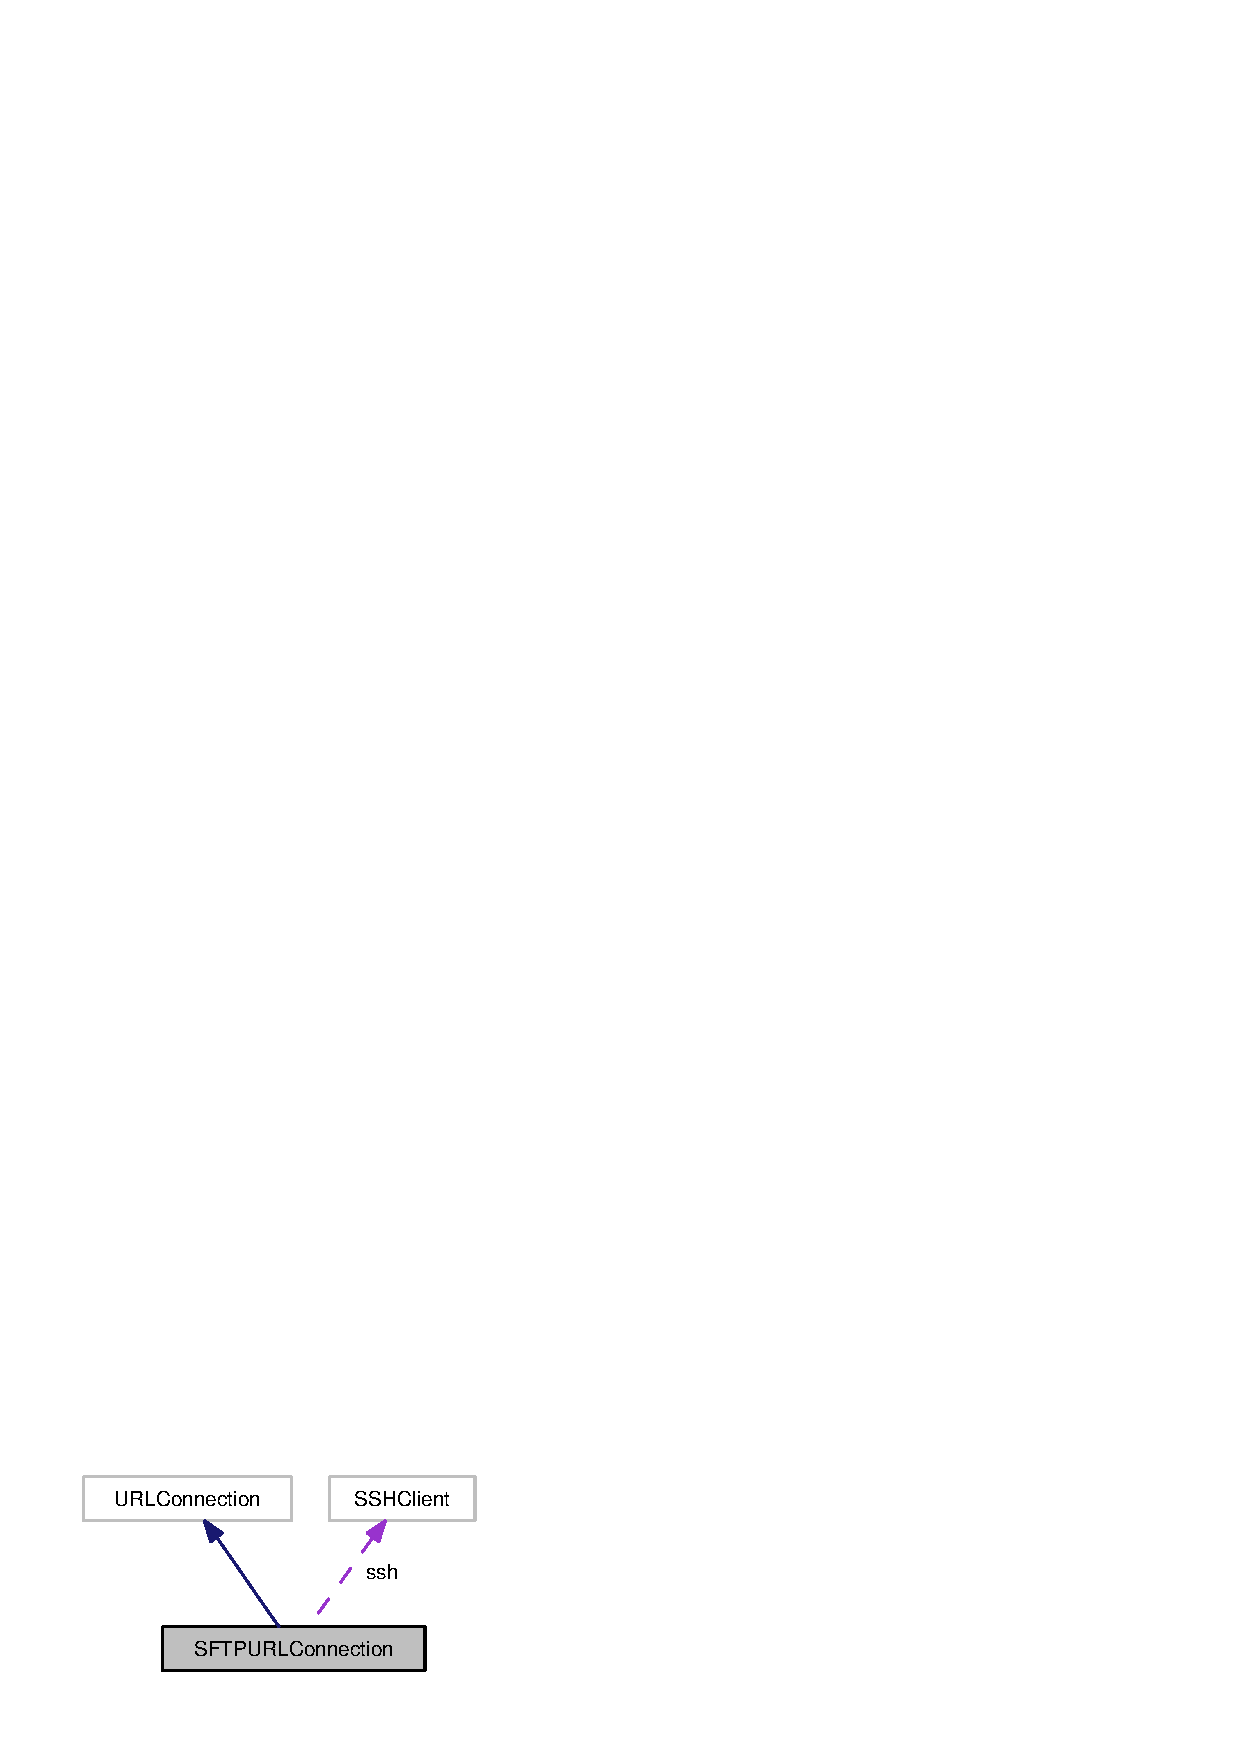
\includegraphics[width=232pt]{classorg_1_1smallfoot_1_1filexfer_1_1sftp_1_1SFTPURLConnection__coll__graph}
\end{center}
\end{figure}
\subsection*{Public Member Functions}
\begin{DoxyCompactItemize}
\item 
{\bfseries S\-F\-T\-P\-U\-R\-L\-Connection} (java.\-net.\-U\-R\-L url)\label{classorg_1_1smallfoot_1_1filexfer_1_1sftp_1_1SFTPURLConnection_a31333738e73c420407fe864e744eb5e3}

\item 
void {\bfseries connect} ()\label{classorg_1_1smallfoot_1_1filexfer_1_1sftp_1_1SFTPURLConnection_a1396bf9b5defe9fa844a63b5cd40ac0e}

\item 
java.\-io.\-Input\-Stream {\bf get\-Input\-Stream} ()
\begin{DoxyCompactList}\small\item\em Stubbed, because there's nothing to send us. \end{DoxyCompactList}\item 
java.\-io.\-Output\-Stream {\bf get\-Output\-Stream} ()
\begin{DoxyCompactList}\small\item\em Stubbed, because there's nothing to send us. \end{DoxyCompactList}\item 
void {\bf set\-Content\-Type} (String ignored)
\begin{DoxyCompactList}\small\item\em Stubbed, because there's no change we want to accept yet. \end{DoxyCompactList}\item 
void {\bf set\-Request\-Header} (String name, String value)
\begin{DoxyCompactList}\small\item\em Stubbed, because there's no change we want to accept yet. \end{DoxyCompactList}\end{DoxyCompactItemize}


\subsection{Detailed Description}


Definition at line 18 of file S\-F\-T\-P\-U\-R\-L\-Connection.\-java.



\subsection{Member Function Documentation}
\index{org\-::smallfoot\-::filexfer\-::sftp\-::\-S\-F\-T\-P\-U\-R\-L\-Connection@{org\-::smallfoot\-::filexfer\-::sftp\-::\-S\-F\-T\-P\-U\-R\-L\-Connection}!get\-Input\-Stream@{get\-Input\-Stream}}
\index{get\-Input\-Stream@{get\-Input\-Stream}!org::smallfoot::filexfer::sftp::SFTPURLConnection@{org\-::smallfoot\-::filexfer\-::sftp\-::\-S\-F\-T\-P\-U\-R\-L\-Connection}}
\subsubsection[{get\-Input\-Stream}]{\setlength{\rightskip}{0pt plus 5cm}java.\-io.\-Input\-Stream get\-Input\-Stream (
\begin{DoxyParamCaption}
{}
\end{DoxyParamCaption}
)\hspace{0.3cm}{\ttfamily [inline]}}\label{classorg_1_1smallfoot_1_1filexfer_1_1sftp_1_1SFTPURLConnection_a0924d1107a459be632532ef34324494e}


Stubbed, because there's nothing to send us. 

Oh how did I get caught in the \char`\"{}\-Royal '\-We'\char`\"{} ? 

Definition at line 55 of file S\-F\-T\-P\-U\-R\-L\-Connection.\-java.

\index{org\-::smallfoot\-::filexfer\-::sftp\-::\-S\-F\-T\-P\-U\-R\-L\-Connection@{org\-::smallfoot\-::filexfer\-::sftp\-::\-S\-F\-T\-P\-U\-R\-L\-Connection}!get\-Output\-Stream@{get\-Output\-Stream}}
\index{get\-Output\-Stream@{get\-Output\-Stream}!org::smallfoot::filexfer::sftp::SFTPURLConnection@{org\-::smallfoot\-::filexfer\-::sftp\-::\-S\-F\-T\-P\-U\-R\-L\-Connection}}
\subsubsection[{get\-Output\-Stream}]{\setlength{\rightskip}{0pt plus 5cm}java.\-io.\-Output\-Stream get\-Output\-Stream (
\begin{DoxyParamCaption}
{}
\end{DoxyParamCaption}
)\hspace{0.3cm}{\ttfamily [inline]}}\label{classorg_1_1smallfoot_1_1filexfer_1_1sftp_1_1SFTPURLConnection_a4170f42681efaf92df5c2030f5298905}


Stubbed, because there's nothing to send us. 

Oh how did I get caught in the \char`\"{}\-Royal '\-We'\char`\"{} ? 

Definition at line 47 of file S\-F\-T\-P\-U\-R\-L\-Connection.\-java.

\index{org\-::smallfoot\-::filexfer\-::sftp\-::\-S\-F\-T\-P\-U\-R\-L\-Connection@{org\-::smallfoot\-::filexfer\-::sftp\-::\-S\-F\-T\-P\-U\-R\-L\-Connection}!set\-Content\-Type@{set\-Content\-Type}}
\index{set\-Content\-Type@{set\-Content\-Type}!org::smallfoot::filexfer::sftp::SFTPURLConnection@{org\-::smallfoot\-::filexfer\-::sftp\-::\-S\-F\-T\-P\-U\-R\-L\-Connection}}
\subsubsection[{set\-Content\-Type}]{\setlength{\rightskip}{0pt plus 5cm}void set\-Content\-Type (
\begin{DoxyParamCaption}
\item[{String}]{ignored}
\end{DoxyParamCaption}
)\hspace{0.3cm}{\ttfamily [inline]}}\label{classorg_1_1smallfoot_1_1filexfer_1_1sftp_1_1SFTPURLConnection_aa608e58be69b0389d82d846a25091d36}


Stubbed, because there's no change we want to accept yet. 

Sorry, apparently \char`\"{}at this time\char`\"{} is more professional, if you listen to the wordy airport announcements.


\begin{DoxyParams}{Parameters}
{\em ignored} & ignored \\
\hline
\end{DoxyParams}


Definition at line 42 of file S\-F\-T\-P\-U\-R\-L\-Connection.\-java.

\index{org\-::smallfoot\-::filexfer\-::sftp\-::\-S\-F\-T\-P\-U\-R\-L\-Connection@{org\-::smallfoot\-::filexfer\-::sftp\-::\-S\-F\-T\-P\-U\-R\-L\-Connection}!set\-Request\-Header@{set\-Request\-Header}}
\index{set\-Request\-Header@{set\-Request\-Header}!org::smallfoot::filexfer::sftp::SFTPURLConnection@{org\-::smallfoot\-::filexfer\-::sftp\-::\-S\-F\-T\-P\-U\-R\-L\-Connection}}
\subsubsection[{set\-Request\-Header}]{\setlength{\rightskip}{0pt plus 5cm}void set\-Request\-Header (
\begin{DoxyParamCaption}
\item[{String}]{name, }
\item[{String}]{value}
\end{DoxyParamCaption}
)\hspace{0.3cm}{\ttfamily [inline]}}\label{classorg_1_1smallfoot_1_1filexfer_1_1sftp_1_1SFTPURLConnection_ac2f45f32dfcaef408189cabb2644841c}


Stubbed, because there's no change we want to accept yet. 

Sorry, apparently \char`\"{}at this time\char`\"{} is more professional, if you listen to the wordy airport announcements.


\begin{DoxyParams}{Parameters}
{\em name} & ignored \\
\hline
{\em value} & ignored \\
\hline
\end{DoxyParams}


Definition at line 35 of file S\-F\-T\-P\-U\-R\-L\-Connection.\-java.



The documentation for this class was generated from the following file\-:\begin{DoxyCompactItemize}
\item 
java/sftp/{\bf S\-F\-T\-P\-U\-R\-L\-Connection.\-java}\end{DoxyCompactItemize}

\section{version Class Reference}
\label{classorg_1_1smallfoot_1_1filexfer_1_1version}\index{version@{version}}


version is used to allow a package that uses this package to be able to \char`\"{}ask\char`\"{} the jar file what version it is  


\subsection*{Static Public Member Functions}
\begin{DoxyCompactItemize}
\item 
static void {\bf main} (String arg[$\,$])
\begin{DoxyCompactList}\small\item\em returns the version of the class; used to cause the build-\/time-\/detected version and buildid to be available by consumers of the generated fctransfer.\+jar file \end{DoxyCompactList}\end{DoxyCompactItemize}


\subsection{Detailed Description}
version is used to allow a package that uses this package to be able to \char`\"{}ask\char`\"{} the jar file what version it is 

Definition at line 10 of file version.\+java.



\subsection{Member Function Documentation}
\index{org\+::smallfoot\+::filexfer\+::version@{org\+::smallfoot\+::filexfer\+::version}!main@{main}}
\index{main@{main}!org\+::smallfoot\+::filexfer\+::version@{org\+::smallfoot\+::filexfer\+::version}}
\subsubsection[{main}]{\setlength{\rightskip}{0pt plus 5cm}static void main (
\begin{DoxyParamCaption}
\item[{String}]{arg[$\,$]}
\end{DoxyParamCaption}
)\hspace{0.3cm}{\ttfamily [inline]}, {\ttfamily [static]}}\label{classorg_1_1smallfoot_1_1filexfer_1_1version_ae4faf7ff4190d227357ef851490d7757}


returns the version of the class; used to cause the build-\/time-\/detected version and buildid to be available by consumers of the generated fctransfer.\+jar file 

for example\+: java -\/cp fctransfer.\+jar \doxyref{org.\+smallfoot.\+filexfer.\+version}{p.}{classorg_1_1smallfoot_1_1filexfer_1_1version} 0.\+3.\+44


\begin{DoxyParams}{Parameters}
{\em arg} & ignored \\
\hline
\end{DoxyParams}


Definition at line 21 of file version.\+java.



The documentation for this class was generated from the following file\+:\begin{DoxyCompactItemize}
\item 
java/{\bf version.\+java}\end{DoxyCompactItemize}

\section{Winch\-Factory Class Reference}
\label{classorg_1_1smallfoot_1_1filexfer_1_1WinchFactory}\index{Winch\-Factory@{Winch\-Factory}}


\doxyref{Winch\-Factory}{p.}{classorg_1_1smallfoot_1_1filexfer_1_1WinchFactory} is the main entry point for this package; Winch\-Factory.\-main() shows how a filetransfer \char`\"{}winch\char`\"{} can be found for a U\-R\-L, but in general a consumer of this class wants to\-:  


\subsection*{Public Member Functions}
\begin{DoxyCompactItemize}
\item 
{\bf Winch\-Factory} ()
\begin{DoxyCompactList}\small\item\em stub constructor for the \doxyref{Winch\-Factory()}{p.}{classorg_1_1smallfoot_1_1filexfer_1_1WinchFactory_ae893b0fc6603239324297b31118fae7d} also appends/writes the system property \char`\"{}java.\-protocol.\-handler.\-pkgs\char`\"{} in accordance with {\tt http\-://docs.\-oracle.\-com/javase/7/docs/api/java/net/\-U\-R\-L.\-html} \end{DoxyCompactList}\end{DoxyCompactItemize}
\subsection*{Static Public Member Functions}
\begin{DoxyCompactItemize}
\item 
static {\bf File\-Transfer\-Winch} {\bf get\-Winch} (String url)  throws java.\-net.\-Malformed\-U\-R\-L\-Exception     
\begin{DoxyCompactList}\small\item\em provides a \doxyref{File\-Transfer\-Winch}{p.}{classorg_1_1smallfoot_1_1filexfer_1_1FileTransferWinch} matching the U\-R\-L given \end{DoxyCompactList}\item 
static {\bf File\-Transfer\-Winch} {\bf get\-Winch} (java.\-net.\-U\-R\-L url)
\begin{DoxyCompactList}\small\item\em provides a \doxyref{File\-Transfer\-Winch}{p.}{classorg_1_1smallfoot_1_1filexfer_1_1FileTransferWinch} matching the U\-R\-L given \end{DoxyCompactList}\item 
static String[$\,$] {\bf get\-Winch\-Examples} (String url)  throws java.\-net.\-Malformed\-U\-R\-L\-Exception     
\begin{DoxyCompactList}\small\item\em provides an array of example U\-R\-Ls based on the given model by iterating all known Winches \end{DoxyCompactList}\item 
static void {\bfseries main} (String[$\,$] args)\label{classorg_1_1smallfoot_1_1filexfer_1_1WinchFactory_a8b260eecbaabcef8473fd87ada040682}

\end{DoxyCompactItemize}
\subsection*{Protected Member Functions}
\begin{DoxyCompactItemize}
\item 
java.\-util.\-Vector\\*
$<$ {\bf File\-Transfer\-Winch} $>$ {\bfseries get\-Winches} ()\label{classorg_1_1smallfoot_1_1filexfer_1_1WinchFactory_a59d46b83cc5f9106aab011bb58b55ecd}

\end{DoxyCompactItemize}
\subsection*{Static Private Attributes}
\begin{DoxyCompactItemize}
\item 
static boolean {\bfseries \-\_\-reg} = false\label{classorg_1_1smallfoot_1_1filexfer_1_1WinchFactory_a22e6581675a84937ebc9ead4c1109570}

\end{DoxyCompactItemize}


\subsection{Detailed Description}
\doxyref{Winch\-Factory}{p.}{classorg_1_1smallfoot_1_1filexfer_1_1WinchFactory} is the main entry point for this package; Winch\-Factory.\-main() shows how a filetransfer \char`\"{}winch\char`\"{} can be found for a U\-R\-L, but in general a consumer of this class wants to\-: 


\begin{DoxyEnumerate}
\item use \doxyref{get\-Winch(\-String)}{p.}{classorg_1_1smallfoot_1_1filexfer_1_1WinchFactory_a1267459debe1139bfc984cd72c915e87} to find an appropriate winch for a U\-R\-L
\item exercise the winch using File\-Transfer\-Winch.\-upload(\-File) or File\-Transfer\-Winch.\-upload(\-String)
\item reap the rewards of not having to re-\/code this functionality 
\end{DoxyEnumerate}

Definition at line 20 of file Winch\-Factory.\-java.



\subsection{Constructor \& Destructor Documentation}
\index{org\-::smallfoot\-::filexfer\-::\-Winch\-Factory@{org\-::smallfoot\-::filexfer\-::\-Winch\-Factory}!Winch\-Factory@{Winch\-Factory}}
\index{Winch\-Factory@{Winch\-Factory}!org::smallfoot::filexfer::WinchFactory@{org\-::smallfoot\-::filexfer\-::\-Winch\-Factory}}
\subsubsection[{Winch\-Factory}]{\setlength{\rightskip}{0pt plus 5cm}{\bf Winch\-Factory} (
\begin{DoxyParamCaption}
{}
\end{DoxyParamCaption}
)\hspace{0.3cm}{\ttfamily [inline]}}\label{classorg_1_1smallfoot_1_1filexfer_1_1WinchFactory_ae893b0fc6603239324297b31118fae7d}


stub constructor for the \doxyref{Winch\-Factory()}{p.}{classorg_1_1smallfoot_1_1filexfer_1_1WinchFactory_ae893b0fc6603239324297b31118fae7d} also appends/writes the system property \char`\"{}java.\-protocol.\-handler.\-pkgs\char`\"{} in accordance with {\tt http\-://docs.\-oracle.\-com/javase/7/docs/api/java/net/\-U\-R\-L.\-html} 

N\-O\-T\-E\-: my own code uses \char`\"{}package1\-:package2\char`\"{} whereas the example uses \char`\"{}package1$\vert$package2\char`\"{} 

Definition at line 88 of file Winch\-Factory.\-java.



\subsection{Member Function Documentation}
\index{org\-::smallfoot\-::filexfer\-::\-Winch\-Factory@{org\-::smallfoot\-::filexfer\-::\-Winch\-Factory}!get\-Winch@{get\-Winch}}
\index{get\-Winch@{get\-Winch}!org::smallfoot::filexfer::WinchFactory@{org\-::smallfoot\-::filexfer\-::\-Winch\-Factory}}
\subsubsection[{get\-Winch}]{\setlength{\rightskip}{0pt plus 5cm}static {\bf File\-Transfer\-Winch} get\-Winch (
\begin{DoxyParamCaption}
\item[{String}]{url}
\end{DoxyParamCaption}
) throws java.\-net.\-Malformed\-U\-R\-L\-Exception\hspace{0.3cm}{\ttfamily [inline]}, {\ttfamily [static]}}\label{classorg_1_1smallfoot_1_1filexfer_1_1WinchFactory_a1267459debe1139bfc984cd72c915e87}


provides a \doxyref{File\-Transfer\-Winch}{p.}{classorg_1_1smallfoot_1_1filexfer_1_1FileTransferWinch} matching the U\-R\-L given 

\begin{DoxyReturn}{Returns}
populated winch based on the U\-R\-L given 
\end{DoxyReturn}

\begin{DoxyExceptions}{Exceptions}
{\em java.\-net.\-Malformed\-U\-R\-L\-Exception} & if the U\-R\-L created form the String is malformed \\
\hline
\end{DoxyExceptions}

\begin{DoxyParams}{Parameters}
{\em url} & U\-R\-L to connect to \\
\hline
\end{DoxyParams}


Definition at line 29 of file Winch\-Factory.\-java.

\index{org\-::smallfoot\-::filexfer\-::\-Winch\-Factory@{org\-::smallfoot\-::filexfer\-::\-Winch\-Factory}!get\-Winch@{get\-Winch}}
\index{get\-Winch@{get\-Winch}!org::smallfoot::filexfer::WinchFactory@{org\-::smallfoot\-::filexfer\-::\-Winch\-Factory}}
\subsubsection[{get\-Winch}]{\setlength{\rightskip}{0pt plus 5cm}static {\bf File\-Transfer\-Winch} get\-Winch (
\begin{DoxyParamCaption}
\item[{java.\-net.\-U\-R\-L}]{url}
\end{DoxyParamCaption}
)\hspace{0.3cm}{\ttfamily [inline]}, {\ttfamily [static]}}\label{classorg_1_1smallfoot_1_1filexfer_1_1WinchFactory_aa260cf55e58230cd670e91507ec4704c}


provides a \doxyref{File\-Transfer\-Winch}{p.}{classorg_1_1smallfoot_1_1filexfer_1_1FileTransferWinch} matching the U\-R\-L given 

\begin{DoxyReturn}{Returns}
populated winch based on the U\-R\-L given 
\end{DoxyReturn}

\begin{DoxyParams}{Parameters}
{\em url} & U\-R\-L to connect to \\
\hline
\end{DoxyParams}


Definition at line 38 of file Winch\-Factory.\-java.

\index{org\-::smallfoot\-::filexfer\-::\-Winch\-Factory@{org\-::smallfoot\-::filexfer\-::\-Winch\-Factory}!get\-Winch\-Examples@{get\-Winch\-Examples}}
\index{get\-Winch\-Examples@{get\-Winch\-Examples}!org::smallfoot::filexfer::WinchFactory@{org\-::smallfoot\-::filexfer\-::\-Winch\-Factory}}
\subsubsection[{get\-Winch\-Examples}]{\setlength{\rightskip}{0pt plus 5cm}static String [$\,$] get\-Winch\-Examples (
\begin{DoxyParamCaption}
\item[{String}]{url}
\end{DoxyParamCaption}
) throws java.\-net.\-Malformed\-U\-R\-L\-Exception\hspace{0.3cm}{\ttfamily [inline]}, {\ttfamily [static]}}\label{classorg_1_1smallfoot_1_1filexfer_1_1WinchFactory_a830bb6d507e304f5562ee9f6b54429a4}


provides an array of example U\-R\-Ls based on the given model by iterating all known Winches 

\begin{DoxyReturn}{Returns}
populated array of examples 
\end{DoxyReturn}

\begin{DoxyParams}{Parameters}
{\em url} & sample U\-R\-L to be used in examples \\
\hline
\end{DoxyParams}

\begin{DoxyExceptions}{Exceptions}
{\em java.\-net.\-Malformed\-U\-R\-L\-Exception} & if the given U\-R\-L chokes on conversion to a java.\-net.\-U\-R\-L \\
\hline
\end{DoxyExceptions}


Definition at line 56 of file Winch\-Factory.\-java.



The documentation for this class was generated from the following file\-:\begin{DoxyCompactItemize}
\item 
java/{\bf Winch\-Factory.\-java}\end{DoxyCompactItemize}

\chapter{File Documentation}
\section{htdocs/\-R\-E\-A\-D\-M\-E.dox File Reference}
\label{README_8dox}\index{htdocs/\-R\-E\-A\-D\-M\-E.\-dox@{htdocs/\-R\-E\-A\-D\-M\-E.\-dox}}

\section{java/sftp/\+Handler.java File Reference}
\label{Handler_8java}\index{java/sftp/\+Handler.\+java@{java/sftp/\+Handler.\+java}}
\subsection*{Data Structures}
\begin{DoxyCompactItemize}
\item 
class {\bf Handler}
\end{DoxyCompactItemize}

\section{java/sftp/\+S\+F\+T\+P\+U\+R\+L\+Connection.java File Reference}
\label{SFTPURLConnection_8java}\index{java/sftp/\+S\+F\+T\+P\+U\+R\+L\+Connection.\+java@{java/sftp/\+S\+F\+T\+P\+U\+R\+L\+Connection.\+java}}
\subsection*{Data Structures}
\begin{DoxyCompactItemize}
\item 
class {\bf S\+F\+T\+P\+U\+R\+L\+Connection}
\end{DoxyCompactItemize}

\section{java/version.java File Reference}
\label{version_8java}\index{java/version.\+java@{java/version.\+java}}
\subsection*{Data Structures}
\begin{DoxyCompactItemize}
\item 
class {\bf version}
\begin{DoxyCompactList}\small\item\em version is used to allow a package that uses this package to be able to \char`\"{}ask\char`\"{} the jar file what version it is \end{DoxyCompactList}\end{DoxyCompactItemize}

\section{java/\-Winch\-Factory.java File Reference}
\label{WinchFactory_8java}\index{java/\-Winch\-Factory.\-java@{java/\-Winch\-Factory.\-java}}

%--- End generated contents ---

% Index
\newpage
\phantomsection
\addcontentsline{toc}{chapter}{Index}
\printindex

\end{document}
